% ****** Start of file apssamp.tex ******
%   This file is part of the APS files in the REVTeX 4 distribution.
%   Version 4.0 of REVTeX, August 2001
%   Copyright (c) 2001 The American Physical Society.
%   See the REVTeX 4 README file for restrictions and more information.
% TeX'ing this file requires that you have AMS-LaTeX 2.0 installed
% as well as the rest of the prerequisites for REVTeX 4.0
% See the REVTeX 4 README file
% It also requires running BibTeX. The commands are as follows:
%  1)  latex apssamp.tex
%  2)  bibtex apssamp
%  3)  latex apssamp.tex
%  4)  latex apssamp.tex
%\documentclass[twocolumn,amsmath,amssymb,10pt,groupedaddress,a4paper]{revtex4}
%\documentclass[preprint,showpacs,preprintnumbers,amsmath,amssymb]{revtex4}
% Some other (several out of many) possibilities
%\documentclass[preprint,aps]{revtex4}
%\documentclass[preprint,aps,draft]{revtex4}
%\documentclass[prb]{revtex4}% Physical Review B
%\documentclass[preprint,aps]{revtex4}
%\documentclass[preprint,eqsecnum,aps]{revtex4}
%\documentclass[eqsecnum,aps]{revtex4}
%\tightenlines
%\usepackage[dvips]{graphicx}
%\usepackage{amssymb}
%\usepackage{floatflt}
%\usepackage{array}
%\begin{document}
% Include figure files
% Align table columns on decimal point
% bold math
%\usepackage{array}
%\usepackage{bibunits}% Separate lists of references
%\usepackage[bookmarksnumbered,colorlinks,backref, bookmarks, breaklinks, linktocpage]{hyperref}
%\setlongtables
%\nofiles


\documentclass[twocolumn,10pt,groupedaddress,letter]{revtex4}
\usepackage{amssymb}
\usepackage{amsmath}
\usepackage{makeidx}
\usepackage[bookmarksnumbered,colorlinks,bookmarks,breaklinks,linktocpage,citecolor=blue]{hyperref}
\usepackage{graphicx}
\usepackage{dcolumn}
\usepackage{bm}
\usepackage{fancyheadings}
\usepackage{pstricks}
\usepackage{longtable}
\usepackage{multirow}
\usepackage[active]{srcltx}

\setcounter{MaxMatrixCols}{10}
%TCIDATA{OutputFilter=Latex.dll}
%TCIDATA{Version=5.00.0.2606}
%TCIDATA{<META NAME="SaveForMode" CONTENT="1">}
%TCIDATA{BibliographyScheme=BibTeX}
%TCIDATA{LastRevised=Monday, August 06, 2007 12:14:03}
%TCIDATA{<META NAME="GraphicsSave" CONTENT="32">}

\pagestyle{fancy}
\textheight 250mm
\topmargin -15mm
\bibliographystyle{ieeetr.bst}
% \input{tcilatex}

\begin{document}

\preprint{Nuclear Data Sheets}
\title{EMPIRE: Nuclear Reaction Model Code System for Data Evaluation}
\author{M. Herman}
\affiliation{National Nuclear Data Center, Brookhaven National Laboratory,
Upton,~NY~11973-5000, USA}
\author{R. Capote}
\affiliation{Nuclear Data Section, International Atomic Energy Agency, Vienna, Austria}
\author{B.V. Carlson}
\affiliation{Instituto Tecnologico de Aeronautica, Sao Jose dos Campos SP, Brazil}
\author{P. Oblo\v zinsk\'y}
\affiliation{National Nuclear Data Center, Brookhaven National Laboratory,
Upton,~NY~11973-5000, USA }
\author{M. Sin}
\affiliation{Nuclear Physics Department, Bucharest University, Bucharest-Magurele, Romania}
\author{A. Trkov }
\affiliation{Jozef Stefan Institute, Ljubljana, Slovenia}
\author{H. Wienke}
\affiliation{Belgonucleaire, B2480, Dessel, Belgium}
\author{V. Zerkin}
\affiliation{Nuclear Data Section, International Atomic Energy Agency, Vienna, Austria\\ }

\received{August 15, 2007}

\begin{abstract}

EMPIRE is a modular system of nuclear reaction codes, comprising various
nuclear models, and designed for calculations over a broad range of energies
and incident particles. A projectile can be a neutron, proton, any ion
(including Heavy Ions) or a photon. The energy range extends from the
beginning of the unresolved resonance region for neutron induced reactions ($%
\backsim$ keV) and goes up to several hundred MeV for Heavy Ion induced
reactions.

The code accounts for the major nuclear reaction mechanisms, including
direct, pre-equilibrium and compound nucleus ones. Direct reactions
are described
by a generalized optical model (ECIS03) or by the simplified coupled
channels approach (CCFUS). The preequilibrium mechanism can be treated by
a deformation dependent Multi-step Direct (ORION + TRISTAN) model,
by a NVWY Multi-step Compound one or by either a preequilibrium exciton model
with cluster emission (PCROSS) or by another with full angular
momentum coupling (DEGAS). Finally, the
compound nucleus decay is described by the full featured Hauser-Feshbach
model with $\gamma $-cascade and width fluctuations. Advanced treatment of
the fission channel takes into account transmission through a
multiple-humped fission barrier with absorption in the wells. The fission
probability is derived in the WKB approximation within the optical model of
fission.

Several options for nuclear level densities include the
EMPIRE-specific approach, which
accounts for the effects of the dynamic deformation of a fast rotating
nucleus, the classical Gilbert-Cameron approach and pre-calculated tables
obtained with a microscopic model based on HFB single-particle level
schemes with collective enhancement.
A comprehensive library of input parameters covers nuclear masses, optical
model parameters, ground state deformations, discrete levels and decay
schemes, level densities, fission barriers, moments of inertia and
$\gamma$-ray strength functions.

The results can be converted into ENDF-6 formatted files using the
accompanying code EMPEND and completed with neutron resonances extracted
from the existing evaluations. The package contains the full
EXFOR (CSISRS) library of experimental reaction data that are automatically retrieved
during the calculations. Publication quality graphs can be obtained using
the powerful and flexible plotting package ZVView. The graphic user
interface, written in Tcl/Tk, provides for easy operation of the system.

This paper describes the capabilities of the code, outlines physical models and
indicates parameter libraries used by EMPIRE to predict reaction cross
sections and spectra, mainly for nucleon induced reactions. Selected applications
of EMPIRE are discussed, the most important being an extensive use of the code in
evaluations of neutron reactions for the new US library ENDF/B-VII.0.
Future extensions of the system are outlined, including neutron resonance module as
well as capabilities of generating covariances, using both KALMAN and Monte Carlo methods,
that are still being advanced and refined.
\\ \vspace{0.5cm} \\
\end{abstract}

\maketitle
\tableofcontents

%\draft
% \title{EMPIRE: Integrated System of Nuclear Reaction Model Codes for Data Evaluation}

% \title{EMPIRE: Integrated Nuclear Reaction Model Code for Data Evaluation}

% \author{S. F. Mughabghab}
% \affiliation{National Nuclear Data Center, Brookhaven National Laboratory, Upton~NY~11973-5000 }

%\author{T. Kawano}
%\affiliation{T-16, Los Alamos National Laboratory, Los Alamos, NM 87545}
% \author{Young-Sik Cho}
% \affiliation{Korea Atomic Energy Research Institute, Nuclear Data Evaluation Lab., Daejeon, Korea}
% \author{D. Rochman}
% \affiliation{National Nuclear Data Center, Brookhaven National Laboratory, Upton~NY~11973-5000- }

\vspace*{12mm} \lhead{EMPIRE: Nuclear Reaction Code...}
\chead{NUCLEAR DATA
SHEETS} \rhead{M. Herman \textit{et al.}} \lfoot{} \rfoot{} %
\setlength{\headrulewidth}{0.4pt} \setlength{\footrulewidth}{0.4pt}

%%%%%%%%%%%%%%%%%%%%%%%%%%%%%%%%%%%%%%%%%%%%%%%%%%%%%%%%%%%%%%%%%%%%%%%%%%%%%%%%%%%%%%%%%%%%%%%%%%%%%%%%%%%%%%%%%%
% \section{ToDo and deficiencies}
%
% \begin{itemize}
% \item gamma-strength functions to be expanded with the new ones, add higher multipolarities
% \item Plots to be improved
% \item Formatting updated with isomeric cross sections and mixed exclusive/inclusive spectra
% \end{itemize}

\newpage

\section{Introduction}

Recent release of the evaluated nuclear data ENDF/B-VII.0 library~\cite%
{ENDF-VII} substantiated the importance of theory in modern evaluation
methodology. Nuclear reaction codes are instrumental in providing
predictions for cross sections and spectra that have not been measured or
need to be interpolated or extrapolated to other energy regions. Use of
theory-based modeling is actually the only viable way of generating
complete and consistent nuclear data files. The most recent, frequently
used, and comprehensive nuclear reaction codes are GNASH~\cite{Young:77,
Young:92, Young:98}, TALYS~\cite{TALYS}, and EMPIRE. This paper is dedicated
to the last of these.

The roots of the EMPIRE nuclear reaction model code originate at the Institute
of Nuclear Research (INR) in Warsaw and can be traced back to the early
seventies, when a vigorous program of activation measurements brought a
natural need for an adequate tool to interpret experimental results. The
ISOMER code~\cite{Grochulski:73} was a first response to this necessity.
This ingenious masterpiece of programming incorporated the spin-dependent
statistical theory of nuclear reactions within the ridiculously small
memory, for
today's standards, of just 4k. ISOMER was coded in ALGOL and ran
on a transistor based computer GIER. The source of the code and input data
were stored on perforated paper tape, which tended to break in the middle
of the night (typical calculations would last an entire weekend). When the new
CYBER-72 (CDC) computer was installed at the INR and the GIER machine was moved
out of the town, a new code became an obvious necessity. Thus, the first
EMPIRE code grew up from this well-prepared, fertile soil, building on the
previous experience with the enthusiasm that characterized research in those
days.

The first version of the EMPIRE code was developed by M. Herman as a part of
his Ph.D. thesis supervised by A. Marcinkowski. The original version,
released in 1980~\cite{EMPIRE-I}, contained the Hauser-Feshbach theory and
the classical HYBRID~\cite{hybrid, hybrid1, hybrid2, hybrid3} model to
account for preequilibrium effects. Width fluctuation corrections were
implemented in terms of the HRTW approach \cite{HRTW,HHM}. Adding the FKK
Multi-step Compound mechanism \cite{FKK} lead to the EMPIRE-MSC version.

In 1985, development of EMPIRE moved, along with the main author, to
ENEA (Bologna). The NVWY~\cite{NVWY} model, another quantum-mechanical
formulation of the Multi-step Compound mechanism, was implemented
in the HMS-EMPIRE version of the code and was
supplemented with the TUL approach\cite{TUL} to Multi-step Direct
emission. This version also included combinatorial calculations of
particle-hole level densities.

\begin{table*}[tbp]
\caption{Major releases of the EMPIRE code. The names of recent releases follow the sequence of victorious
battles of Napoleon Bonaparte in Italy.}
\label{tab:emp-history}%
\begin{tabular}{lrll}
\hline
\textbf{Version} & \textbf{\ Year } & \textbf{Location} & \textbf{Comments}
\\ \hline
EMPIRE & 1980 & Warsaw & CN+HYBRID \\
EMPIRE MSC & 1983 & Warsaw & FKK(MSC) \\
EMPIRE HI & 1988 & Messina & Heavy Ion version \\
EMPIRE HMS & 1991 & Bologna & NVWY(MSC)+TUL(MSD) \\
EMPIRE-2.13 & 2001 & Vienna & totally rewritten \\
EMPIRE-2.17 (Montenotte) & 2002 & Vienna & ECIS, HRTW, EXFOR, HMS, \\
&  &  & DEGAS, RIPL-2, plotting \\
EMPIRE-2.18 (Mondovi) & 2002 & Vienna &  \\
EMPIRE-2.19 (Lodi) & 2005 & Brookhaven & advanced fission, \\
&  &  & photo-nuclear reactions, \\
&  &  & PE clusters (PCROSS), \\
&  &  & OMP fitting, \\
&  &  & merging resonances, \\
&  &  & mixed inclusive/exclusive spectra, \\
&  &  & checking codes, NJOY support, \\
&  &  & used for ENDF/B-VII.0 \\
EMPIRE-3.0 (Arcola) & 2007 & Brookhaven & deformed TUL(MSD) \\
&  &  & Monte Carlo sampling of input parameters \\
&  &  & improved fission \\
&  &  & formatting of isomers \\ \hline
\end{tabular}%
\end{table*}

In addition, a version for Heavy Ion induced reactions (EMPIRE HI) was
developed as a part of the fusion-fission studies carried out in
collaboration with the INFN group at Messina lead by G. Giardina. During
this exercise it became clear that the original formulation did not lend
itself to large scale extensions and a new code would have to be written from
scratch. Thus, interpretation of Heavy Ion (HI) induced reaction data was
the initial motivation for the development of the new EMPIRE-2 code. Its
design was, therefore, guided by the particular necessities of HI
reactions, which posed a
broader variety of challenges than neutron activation. However, these
challenges were exploited to enrich the code and make it more general
without compromising its capabilities for treating neutron induced reactions,
which remained one of its principal objectives.

Actual coding was preceded by a conceptual study to define goals, means and
coding style. It indicated essential features that the new code should
fulfill:

\begin{itemize}
\item be reasonably complete in terms of reaction channels, observables and
applied nuclear reaction models;

\item be flexible in terms of treating different projectiles in a wide range
of incident energies;

\item be easy to use by simplifying input through use of built-in defaults
and input parameter libraries;

\item be open for adding new nuclear reaction models through a modular
structure;

\item provide a full sequence of operations up to the generation of the
ENDF-6 formatted file and comparison plots with automatically retrieved
experimental data.
\end{itemize}

In addition, a set of coding rules was established to simplify programming,
improve readability of the code, increase robustness and facilitate
extensions. Initial development strictly followed these rules. Later it was
decided to incorporate into EMPIRE some well tested third party codes or
routines to speed up development and ensure quality of the results.
Inevitably, the strict coding rules had to be relaxed in such cases but it
has been sought to preserve it as much as possible.

In the early nineties, the EMPIRE developer team was formed when R. Capote
undertook the task of upgrading the optical model part of the code and A.
Trkov became responsible for the ENDF-6 formatting and all related issues.
Eventually, Capote's role in the development of the physics core of EMPIRE
grew to cover multiple aspects, such as direct reactions (CC and
DWBA), the interface to RIPL, the preequilibrium exciton model and,
recently, an advanced
implementation of fission and a global vision of the system.

In 1997 the EMPIRE home site was transferred to the IAEA in Vienna. This move
accelerated development, with two new members joining the team - V.
Zerkin, who implemented EXFOR retrieval and interactive plotting
while P. Oblo\v
zinsk\'y incorporated the exciton model with angular momentum coupling (DEGAS)
and took the lead in promoting EMPIRE internationally. The code was first
officially released (version 2.13)~\cite{EMPIRE:Trieste01} in 2000 on the
occasion of the ICTP Workshop on Nuclear Reaction Data and Nuclear Reactors
in Trieste.

In 2003 EMPIRE found a new home at the National Nuclear Data Center at
BNL (M. Herman and P. Oblo\v{z}insk\'{y}) while R. Capote, A. Trkov and V.
Zerkin continued development in Vienna. M. Sin joined the team bringing
much needed fission expertise and took the lead in a radical upgrade of the
fission channel. B.V. Carlson followed with addition of the photo-nuclear
reactions and highly automatized fitting of the optical model potential.
More recently, H. Wienke upgraded the MSD module by extending it to
deformed nuclei. In Tab.\ref{tab:emp-history} we list the most important
releases of EMPIRE and indicate major additions or modifications with
respect to the previous version.

In this paper we describe the 3.0 version of the code (denominated
'Arcola'). Its immediate predecessor 2.19 was extensively used in the
development of the ENDF/B-VII.0 library~\cite{ENDF-VII}. The following
sections outline physics built into various modules of the EMPIRE
code, contents
of the input libraries, particular features offered by the code and
summarize usage of EMPIRE in various laboratories. The intention of this
write-up is to present capabilities of the system and explain the means it
uses to produce answers. Even with the relatively generous space available
to this review, it is not possible to document all minor features and details
of the algorithms used in the code. In particular, input preparation and
operation of the code are outside the scope of the present paper. Users are
advised to consult the EMPIRE manual available at www.nndc.bnl.gov/empire and
www-nds.iaea.org/empire for more practical instructions. Similarly, we refer
to the RIPL-2 documentation~\cite{RIPL2} for particulars regarding this input
parameter library and to Ref.~\cite{Mughabghab:06} for details
concerning the evaluation of neutron resonances.

\section{Overview of the EMPIRE System}

The current 3.0 version of EMPIRE is a milestone in the evolution of the
EMPIRE system. It marks the point at which the code has achieved practically
all goals that were set up in the conceptual design. We stress again that
EMPIRE-3.0 has been a totally new development although it has benefited from
the experience gained with the previous editions. The code has been
rewritten using more advanced programming concepts. It has been designed to
be general and flexible, and can be applied to the calculation of neutron
capture in the keV region, as well as to Heavy Ion (HI) induced reactions at
several hundreds of MeV. The aim is to provide a powerful environment for
modeling nuclear reactions that can be used in basic research as well as for
the generation of evaluated nuclear data files. To achieve this goal we
implement in a single system an extensive set of models that cover all
the most
important nuclear reaction mechanisms up to the threshold for pion
production. These models provide a complete set of reaction channels and
observables that might be of interest in nuclear applications. Included are
cross sections, spectra, angular distributions and angle-energy correlated
spectra (double-differential cross sections) for nucleons, $\alpha $%
-particles, light ions and $\gamma $-rays, as well as cross sections
for the
population of isomeric levels (activation cross sections). Such extensive
calculations require a considerable number of input parameters. To provide
them, EMPIRE incorporates a comprehensive library of model parameters,
largely based on the IAEA RIPL-2~\cite{RIPL2} project, although the
preliminary recommendations of the follow up edition (RIPL-3) are used when
available. The calculated results can be plotted and compared against
experimental data automatically extracted from the EXFOR library~\cite{EXFOR}%
.

\begin{figure*}[htbp]
\scalebox{0.80}{\includegraphics{flowchart.eps}}
\caption{Flow-chart of the EMPIRE system showing major components of the
system and their interdependence.}
\label{fig:empire-flowchart}
\end{figure*}

The entire EMPIRE system can be divided into five major components:

\begin{enumerate}
\item physics core,

\item input parameter library,

\item scripts and Graphic User Interfaces (GUI),

\item utility codes,

\item library of neutron resonances,

\item library of experimental data (EXFOR).
\end{enumerate}

The flowchart shown in Fig.~\ref{fig:empire-flowchart} illustrates the
organization of the system and indicates the flow of the data. The physics core,
supported by the input parameter library, is the heart of the system. It
consists of a number of modules written in FORTRAN that implement various
nuclear reaction models. Furthermore, the package includes a number
of stand-alone utility codes that are listed in Sec.~\ref{Sec:utility-codes}%
. This significant part of the EMPIRE system serves the particular needs of
nuclear data evaluation, such as ENDF-6 formatting, file verification,
preprocessing, plotting and the ultimate check consisting in processing the
file with the NJOY code~\cite{MacFarlane:06,MacFarlane:94}. The utility
codes, scripts and GUIs are instrumental in making EMPIRE user friendly. Due
to the high level of integration between various components of EMPIRE
provided by the scripts and the intuitive control ensured by the GUIs, the
operation of the whole system is very easy. Most intermediate steps are
completely invisible to the user. In the extreme case of accepting all
defaults, a complete ENDF-6 formatted file, including graphical comparison
with experimental data and full verification with the checking codes, can be
created by typing in the atomic and mass numbers for the target followed by
a couple of mouse-clicks.

We strive to provide ultimately all functionalities necessary or useful for
nuclear data evaluation. The three recent extensions bring us closer to this
goal. The highly automated module for adjustment of optical potential
parameters refines essential parameters underlying any evaluation. The
resonance module, being developed together with Young-Sik Cho, brings the
capability of extracting, analyzing and formatting resonance parameters from
Mughabghab's Atlas of Neutron Resonances~\cite{Mughabghab:06}. The
covariance module enables the quantification of nuclear data uncertainties using
both Monte Carlo and KALMAN methods to combine experimental covariances with
the model based ones. The KALMAN approach uses the original coding by Kawano~%
\cite{Kawano:97} and has been intensively assessed by Rochman and Pigni. The
resonance and covariance extensions, although well advanced, are still in a
phase of development and testing. Therefore, we will only mention them
shortly in the present paper.

We are pleased to acknowledge the existence of similar all-in-one codes that
built on comparable physics, use similar design concepts, aim at analogous
targets and address like users. We mention first the TALYS code~%
\cite{TALYS}, the original development by the Dutch-French collaboration
lead by Koning, and the McGNASH code - being developed at Los Alamos by
Chadwick and Talou as the successor to the well known and widely used GNASH
code~\cite{Young:77, Young:92, Young:98} written by Young and Chadwick. We
are also aware of two independent activities carried out at JAEA in
Japan. This healthy and friendly competition is a sign of the vigor of
the field and should bring considerable benefits. The codes differ in the
selection of the reaction models, tend to employ somewhat different
implementations, and provide unique features that make them better tailored
to particular problems. The comparison of calculated results provides
insight into accuracies of the models and the approximations involved in their
implementation and, last but not least, it helps in the discovery and correction
of coding errors that otherwise would be difficult to detect ("errare humanum
est perseverare diabolicum" Lucius Annaeus Seneca, ca. 4 BC $-$ AD 65).

\section{Physics Core of EMPIRE}

\begin{figure*}[htbp]
\scalebox{0.27}{\includegraphics{Diagram1.eps}}
\caption{Flow-chart of the EMPIRE physics core. Input files and libraries
are indicated in blue, nuclear reaction models in red and
final results in green. The schematic flow of the data is shown in grey.}
\label{fig:physics-core}
\end{figure*}

The physics core of EMPIRE is a combination of the original coding and of
several codes written by other authors. The latter were converted into
subroutines and adapted for their present use. In most cases, the
modifications concerned the input/output interface and never affected the
physical model contained in the original source. The following codes are
incorporated in the physics core of the EMPIRE:

\begin{description}
\item[\textbf{ECIS03%
\index{ECIS}}] Coupled-Channels\index{Coupled-Channels} and DWBA\index{DWBA} code by J. Raynal~\cite{ECIS},

\item[\textbf{CCFUS%
\index{CCFUS}}] simplified Coupled-Channels calculation of HI fusion cross section by C.H. Dasso and S. Landowne~\cite{CCFUS},

\item[\textbf{ORION%
\index{ORION}~\&~TRISTAN%
\index{TRISTAN}}] TUL\index{TUL}~\cite{TUL} approach to Multi-step Direct\index{MSD} by H. Lenske~\cite{ORTRI},

\item[\textbf{DEGAS%
\index{DEGAS}}] exciton model with angular momentum conservation and $\gamma $ emission~\cite{Degas} by E. B\v{e}tak and P. Oblo\v{z}insky,

\item[\textbf{DDHMS%
\index{DDHMS}}] Monte Carlo simulation of the preequilibrium decay by M.B. Chadwick~\cite{DDHMScode}

\item[\textbf{BARMOM%
\index{BARMOM}}] fission barriers and moments of inertia by A. Sierk~\cite{sierk}.
\end{description}

The reader is referred to the original papers for a more detailed
description of these codes.

The selection of the reaction models is pragmatic - we try to cover all
important features of nuclear reactions using modern, physically sound
theoretical approaches that are computationally reasonable. Accordingly, we
employ the Distorted Wave Born Approximation (DWBA) and Coupled-Channel (CC)
methods to be able to deal with deformed nuclei, classical and
quantum-mechanical preequilibrium models to account for precompound effects
at higher incident energies, and a sophisticated approach to fission in
order to describe the structure in the neutron induced fission cross sections of
actinide nuclei. The major part of the incoming flux is treated in terms of
the Hauser-Feshbach formalism, taking into account width fluctuation effects. On
the other hand, we put aside certain highly advanced formulations that would
result in prohibitively lengthy or complex calculations (e.g., the
triple-integral approach to width fluctuations, microscopic calculations of
input quantities, exact treatment of the compound nucleus reactions in
presence of strong direct channels, etc.). These advances will
hopefully become part of the EMPIRE in future but their inclusion in the
current version would not be practical for a general user. Nevertheless,
certain input parameters obtained using microscopic theories are tabulated
and made available to EMPIRE through the RIPL library.

The physics core of EMPIRE retrieves model parameters and performs all
reaction calculations using models specified in an input file. Fig.~\ref%
{fig:physics-core} shows the sequence of calculations and a simplified flow of
the data. The first module reads an input file with the specification of a
reaction and retrieves all model parameters necessary for the calculations.
It assembles a list of involved nuclei and applies appropriate defaults to
the options that were not specified in the input file. Finally, it computes
a number of physical quantities such as level densities, fission barriers,
reaction Q-values, optical model parameters and others. Next, the optical
model is invoked to calculate transmission coefficients for all ejectiles
from each of the decaying nuclei. In the case of an incident nucleon or
Light Ions with A$\leq$4, the optical model is also used for the absorption
(reaction) cross section. Depending on the target this calculations can be
performed in terms of the spherical optical model, the Coupled Channel
model or the Distorted
Wave Born Approximation. Various alternative options are available for
estimating HI fusion.

The unusual feature of EMPIRE is a set of five preequilibrium (PE) modules
that are used to treat the emission of particles, clusters and $\gamma $'s from
the composite nucleus before it reaches the thermal equilibrium of the
compound nucleus. This mechanism gains importance at nucleon incident
energies of the order of 10 MeV and its role increases with energy. The five
PE modules incorporated in EMPIRE include two quantum-mechanical
formulations (MSD and MSC) and three classical approaches (exciton model
DEGAS and PCROSS, and the Monte Carlo simulation (DDHMS)). The presence of so
many PE modules is due to the fact that each of these approaches has certain
advantages but none is perfect. The comparison shown in Table~\ref%
{tbl:PEcapabilities}, demonstrates that no module provides a full set of
features. Therefore, the selection of the optimal model depends on the
application. For example, reactions induced by high energy nucleons ($>$50
MeV) will be most adequately described with the DDHMS module that is the
only one to properly account for the multi-particle PE emission. On the other
hand, lack of exclusive spectra excludes this model from nuclear data
evaluations. We note also that the MSC formalism must be used together with
the MSD and is, therefore, indirectly affected by the shortcomings of the
latter. In order to maximize advantages, EMPIRE allows for the simultaneous use
of several models. In such a case, an internal set of rules is invoked to
select the best partial results and to avoid double-counting (e.g., MSD
inelastic scattering will overwrite contributions from any other model).

\begin{table*}[tbp]
\caption{Capabilities of EMPIRE preequilibrium modules. The '+/-' sign
indicates that the feature is implemented in an approximate way or via
phenomenological systematics.}
\label{tbl:PEcapabilities}%
\begin{tabular}{lccccc}
\hline
\textbf{Feature} & \textbf{MSD } & \textbf{\ MSC } & \textbf{\ DEGAS } &
\textbf{\ PCROSS } & \textbf{\ DDHMS } \\ \hline
Quantum-mechanics & + & + & - & - & - \\
Collective inelastic scattering & + & - & - & - & - \\
Angular momentum coupling & +/- & +/- & + & - & + \\
Angular distributions & + & - & - & +/- & + \\
Charge-exchange reactions & - & + & + & + & + \\
Cluster emission & - & - & - & + & - \\
$\gamma$ emission & - & + & + & + & - \\
Multi-particle PE emission & +/- & - & - & - & + \\
Photo-nuclear reactions & - & - & - & + & + \\
Complex projectile & - & + & - & + & - \\
Exclusive spectra & + & + & + & + & - \\ \hline
\end{tabular}%
\end{table*}

The incident flux absorbed into the composite nucleus is propagated through
the PE mechanisms which populate the continua of the residual nuclei (in case of
emission) or pass the flux to the compound nucleus. These spin and
parity dependent populations are then the starting point for the
Hauser-Feshbach calculations (see Fig.~\ref{fig:physics-core}). In typical
neutron induced reactions at 20 MeV this statistical contribution is about
70\% of the absorption cross section and increases for lower energies. The
Hauser-Feshbach implementation includes multi-particle emission, a
detailed $\gamma $-ray cascade, several options for $\gamma $-ray strength
function and involves various formulations of level densities (including the
approach specific to the EMPIRE code). At low incident energies, typically
below 5 MeV, the Hauser-Feshbach model is replaced by the HRTW formalism
that accounts for the correlations between incident and outgoing channels in
the compound elastic.

The fission channel is an integral part of the Hauser-Feshbach module. It
incorporates fundamental features of fission observed experimentally and
predicted by theoretical studies. Several unique features make the formalism
suitable for basic research and data evaluation. It describes multi-chance
fission induced by light particles and photons, modeling the transmission
through the multi-humped fission barriers within the optical model for
fission concept. This formalism can successfully reproduce the resonant
structure of the fission cross section in the sub-threshold region and is
capable of treating multi-modal fission.

Fig.\ref{fig:physics-core} illustrates how particular cross sections and
spectra are constructed by adding contributions from different reaction
mechanisms. For example, the inelastic scattering cross sections are
generally obtained by summing up the direct reaction, MSD and
Hauser-Feshbach contributions unless the user chooses to exclude direct reaction
and/or PE calculations.

% In the following, we describe particular components of the physics core of the EMPIRE system in more details.

\subsection{Elastic Scattering, Direct Reactions and Fusion}

EMPIRE uses the well known and highly respected code ECIS03 \cite{ECIS} to
perform generalized optical model calculations of elastic scattering and
direct reactions induced by light particles of mass A$\leq$4. The
implementation features automatic preparation of the ECIS03 input. The
transmission coefficients from the optical model calculations are
subsequently used to calculate the fusion cross section. For heavy ions (HI)
and photons, scattering and direct reactions are not taken into account and
other approaches are used to calculate the cross section for fusion.

\subsubsection{The Spherical Optical Model\label{sec:sph-opt}}

In its default mode, for projectiles of mass A$\leq$4, EMPIRE uses ECIS03 to
perform a spherical optical model calculation and uses the RIPL%
\index{RIPL}-2 \cite{RIPL2} optical model segment to obtain the potential
parameters. A typical calculation proceeds roughly as follows.

The scattering wave function of a particle of spin $s$ is expanded in
partial waves as
\begin{equation}
\Psi=%
\frac{4\pi}{kr}\sum_{ljn}\, i^{l}\, e^{i\sigma_{l}}\psi_{l}^{j}(r){\mathcal{Y%
}}_{ls}^{jn}(\hat{r}){\mathcal{Y}}_{ls}^{jn\dagger}(\hat{k})\,,
\label{parwav}
\end{equation}
in terms of the spin-angular functions
\begin{equation}
{\mathcal{Y}}_{ls}^{jn}(\hat{r})=i^{l}\sum_{m\nu}\left\langle s\nu
lm|jn\right\rangle Y_{lm}(\hat{r})\left|s\nu\right\rangle \,,
\end{equation}
where $l$ and $j$ are the orbital and total angular momenta and $%
\left|s\nu\right\rangle $ is an eigenvector of the particle spin. In the
expansion of the wave function, $\sigma_{l}$ is the Coulomb phase, $\hat{r}$
denotes the angular variables and $\hat{k}$ the direction of the incident
momentum.

When the partial wave expansion is substituted in the optical Schroedinger
equation, an independent equation is obtained for the wave function $%
\psi_{l}^{j}$ in each partial wave,
\begin{eqnarray}
\left\{ \frac{d^{2}}{dr^{2}}\right. & - & \frac{l(l+1)}{r^{2}}+k^{2}
\label{eqlj} \\
& - & \left.\frac{2\mu}{\hbar^{2}}\left(U_{cen}(r)+d_{l}^{j}\,
U_{so}(r)\right)\right\} \psi_{l}^{j}(r)=0\,,  \notag
\end{eqnarray}
where $U_{cen}$ and $U_{so}$ are the central and spin-orbit terms of the
phenomenological optical model potential and $%
d_{l}^{j}=(j(j+1)-l(l+1)-s(s+1))/2$

The incoming-wave boundary condition requires that the wave function
asymptotically take the form of an incoming plane wave and an outgoing
scattering wave. The wave function $\psi_{l}^{j}$ must then have the
asymptotic form,
\begin{equation}
\psi_{l}^{j}(r)\rightarrow\frac{i}{2}\left(H_{l}^{-}(r)-H_{l}^{+}(r)e^{2i%
\sigma_{l}}S_{l}^{j}\right)e^{-i\sigma_{l}}\,,  \label{exlj}
\end{equation}
where the $H_{l}^{\pm}(r)$ are the Coulomb wave functions that
asymptotically contain only incoming ($H_{l}^{-}$) or outgoing ($H_{l}^{+}$)
waves. $S_{l}^{j}$ is the nuclear part of the S-matrix element and $%
e^{2i\sigma_{l}}$ the Coulomb phase factor.

The S-matrix elements, $S_{l}^{j}$, are obtained by solving the differential
equation for each partial wave, Eq.~(\ref{eqlj}), in the internal region out
to a matching radius, $r_{m}$, beyond which the optical potential is
negligible. There, the solution and its derivative are matched to the
external wave function, given by Eq.~(\ref{exlj}), and to its derivative.
The calculation is stopped when the S-matrix elements are sufficiently close
to one. For partial waves of larger $l$, the scattering then reduces to pure
Coulomb scattering (or for neutrons, no scattering at all).

When the asymptotic form of the partial wave function, $\psi_{l}^{j}$, of
Eq.~(\ref{exlj}), is substituted in the partial wave expansion of the total
wave function, Eq.~(\ref{parwav}), and the result is compared to the
expected form of the asymptotic wave function, one can extract the partial
wave expansion of the scattering amplitudes,
\begin{eqnarray}
f_{\nu^{\prime}\nu}(\theta) &=& \frac{4\pi}{2ik}\sum_{{{{ljn}{\ mm^{\prime}}}%
}}\;e^{2i\sigma_{l}}\left(S_{l}^{j}-1\right) \notag \\
&& \times Y_{lm^{\prime}}(\hat{r})Y_{lm}^{*}(\hat{k})\left\langle
lm^{\prime}s\nu^{\prime}|jn\right\rangle \left\langle jn|lms\nu\right\rangle.
\end{eqnarray}
Due to the slow convergence of the Coulomb term, these are written in a form
in which the Coulomb contribution has been summed exactly,%
\begin{eqnarray}
f_{\nu^{\prime}\nu}(\theta) & = & \delta_{\nu^{\prime}\nu}\, f_{C}(\theta) \\
& & +\frac{4\pi}{2ik}\sum_{{{ljn\atop mm^{\prime}}}}\;
e^{2i\sigma_{l}}\left(S_{l}^{j}-1\right)\; Y_{lm^{\prime}}(\hat{r}%
)Y_{lm}^{*}(\hat{k})  \notag \\
& & \qquad\qquad\times\left\langle lm^{\prime}s\nu^{\prime}|jn\right\rangle
\left\langle jn|lms\nu\right\rangle \,,  \notag
\end{eqnarray}
where
\begin{equation}
f_{C}(\theta)=-\frac{\eta}{2k\sin^{2}\theta/2}\exp\left[-i\eta\log\left(%
\sin^{2}\theta/2\right)+2i\sigma_{0}\right]
\end{equation}
is the Coulomb amplitude and $\eta=\mu Z_p Z_t e^2/\hbar^2 k $ is the
Sommerfeld parameter.

For spin-0 particles, there is only one amplitude,
\begin{eqnarray}
f(\theta)=f_{00}(\theta) & = & f_{C}(\theta) \\
& + & \frac{1}{2ik}\sum_{l}\;(2l+1)e^{2i\sigma_{l}}(S_{l}^{l}-1)P_{l}(\cos%
\theta)\,.  \notag
\end{eqnarray}

For spin-1/2 particles there are two amplitudes,
\begin{eqnarray}
A(\theta) & = & f_{\frac{1}{2}\frac{1}{2}}=f_{-\frac{1}{2}-\frac{1}{2}} \\
& = & f_{C}(\theta)+\frac{1}{2ik}\sum_{l}\; e^{2i\sigma_{l}}P_{l}(\cos\theta)
\notag \\
& & \qquad\times\left[(l+1)(S_{l}^{l+\frac{1}{2}}-1)+l(S_{l}^{l-\frac{1}{2}%
}-1)\right]  \notag
\end{eqnarray}
and
\begin{eqnarray}
B(\theta) & = & f_{\frac{1}{2}-\frac{1}{2}}=f_{-\frac{1}{2}\frac{1}{2}} \\
& = & \frac{1}{2ik}\sum_{l}\; e^{2i\sigma_{l}}\left[S_{l}^{l+\frac{1}{2}%
}-S_{l}^{l-\frac{1}{2}}\right]P_{l}^{1}(\cos\theta)\,.  \notag
\end{eqnarray}

The differential elastic cross section for an unpolarized incident beam is
obtained by averaging the squared magnitude of the scattering amplitudes
over the initial values of the projectile spin and summing over the final
ones. The general expression that results is
\begin{equation}
\frac{d\sigma}{d\Omega}=\frac{1}{2s+1}\sum_{\nu\nu^{\prime}}\left|f_{\nu^{%
\prime}\nu}(\theta)\right|^{2}\,.  \label{difel}
\end{equation}
For spin-0 particles, this is
\begin{equation}
\frac{d\sigma}{d\Omega}=\left|f(\theta)\right|^{2}\qquad\qquad s=0\,.
\end{equation}
For spin-1/2 particles, it is
\begin{equation}
\frac{d\sigma}{d\Omega}=\left|A(\theta)\right|^{2}+\left|B(\theta)%
\right|^{2}\qquad\qquad s=1/2\,.
\end{equation}

For particles of spin-1/2 and greater, one can define vector and tensor spin
observables in terms of other combinations of the amplitudes. In particular,
for particles of spin-1/2, the vector polarization, $P(\theta)$, is
\begin{equation}
P(\theta)=\frac{2\,\text{Im}\, A^{*}(\theta)B(\theta)}{d\sigma/d\Omega}\,.
\end{equation}

The fraction of flux absorbed from each partial wave is given by the
transmission coefficient, $T_{l}^{j}$, defined as
\begin{equation}
T_{l}^{j}=1-\left|S_{l}^{j}\right|^{2}\,.
\end{equation}
These are simplified for later use in HF calculations by eliminating their $%
j $ dependence,
\begin{equation}
T_{l}=\frac{1}{(2s+1)(2l+1)}\sum_j (2j+1) T_{l}^{j}\,.
\end{equation}
The reaction and absorption cross sections, which are identical here, can be
expressed in terms of the transmission coefficients as
\begin{equation}
\sigma_{r}=\frac{1}{2s+1}\frac{\pi}{k^{2}}\sum_{lj}\;(2j+1)\, T_{l}^{j}\,.
\end{equation}

For charged particles, integration of the differential elastic cross section
of Eq.~(\ref{difel}) leads to an infinite result, due to the infinite range
of the Coulomb interaction. For neutrons, it yields the shape elastic cross
section,
\begin{equation}
\sigma_{el}=\int\; d\Omega\;\frac{d\sigma}{d\Omega}=\frac{\pi}{2k^{2}}%
\sum_{lj}\;(2j+1)\left|1-S_{l}^{j}\right|^{2}\,.
\end{equation}

For neutrons, the total cross section is defined as the sum of the elastic
and reaction cross sections,
\begin{equation}
\sigma_{tot}=\sigma_{el}+\sigma_{r}=\frac{\pi}{k^{2}}\sum_{lj}(2j+1)(1-\text{%
Re}\, S_{l}^{j})\,.
\end{equation}
The total cross section takes into account all flux lost from the incident
plane wave, either by scattering or by absorption.

\subsubsection{The Deformed Optical Model\label{sec:DWBA-CC}}

Coupled-channel (CC) calculations are important for modeling reactions on
deformed nuclei and, in particular, for the correct description of the strong
population of collective discrete levels in inelastic scattering.
Symmetric rotational, vibrational-rotational and harmonic-vibrational CC
modes are available in the EMPIRE implementation of ECIS03. The
implementation also features automatic preparation of the ECIS03 input. It
uses the RIPL%
\index{RIPL}-2 \cite{RIPL2} optical model segment and resorts to the RIPL-2
discrete level schemes and to the RIPL-2 deformation parameters (quadrupole
deformations $\beta _{2}$) only if these are not included in the optical
model parameter set available from RIPL-2. The vibrational (dynamic)
deformations are defined as 0.15 for quadrupole and 0.05 for octupole
vibrations. Calculations can be performed for the majority of deformed
nuclei including rotational and vibrational ones, even-even and even-A
ones with integer spins, as well as odd-A ones with half-integer spins.

The partial wave expansion proceeds in the CC optical model much as it did
in the single-channel one. There are several new features however. The first
of these is that the excited states and their angular momentum must now be
taken into account.

The spin-angular functions are coupled to the target states to form
target-spin-angular functions,
\begin{equation}
{\mathcal{Y}}_{lsjc}^{JM}(%
\hat{r})=\sum_{nN_{c}}\,\left\langle jnI_{c}N_{c}|JM\right\rangle {\mathcal{Y%
}}_{ls}^{jn}(\hat{r})\left|I_{c}N_{c}\right\rangle \,,
\end{equation}
where the $\left|I_{c}N_{c}\right\rangle $ represent the target states with
total angular momentum and angular momentum projection $I_{c}$ and $N_{c}$,
respectively.

The scattering wave function is expanded in a sum over both the excited
states and the angular momenta,
\begin{equation}
\Psi=4\pi\sum_{{{ljcJM\atop l^{\prime}j^{\prime}c^{\prime}}}}\;{\mathcal{%
Y}}_{l^{\prime}sj^{\prime}c^{\prime}}^{JM}(\hat{r})i^{l^{\prime}}\psi_{l^{%
\prime}j^{\prime}c^{\prime},ljc}^{J}(r)\frac{e^{i\sigma_{lc}}}{k_{c}r}{%
\mathcal{Y}}_{lsjc}^{JM\dagger}(\hat{k})\,.  \label{cpar}
\end{equation}
The wave functions, $\psi_{l^{\prime}j^{\prime}c^{\prime},ljc}^{J}(r)$,
couple different values of the angular momenta $l$ and $j$ and different
channels $c$ for each value of the total angular momentum $J$. The Coulomb
phase now depends on the channel energy, through $k_{c}$, as well as on the
angular momentum.

When the partial-wave expansion of the wave function is substituted in the
optical Schroedinger equation, the latter can be reduced to a set of coupled
equations for each value of the total angular momentum $J$. These are
\begin{eqnarray}
\frac{\hbar^{2}}{2\mu}\left\{ \frac{d^{2}}{dr^{2}}\right. & - & \left.\frac{%
l^{\prime}(l^{\prime}+1)}{r^{2}}+k_{c^{\prime}}^{2}\right\}
\psi_{l^{\prime}j^{\prime}c^{\prime},ljc}^{J}(r) \\
& - & \sum_{l^{\prime\prime}j^{\prime\prime}c^{\prime\prime}}\;{\mathcal{U}}%
_{l^{\prime}j^{\prime}c^{\prime},l^{\prime\prime}j^{\prime\prime}c^{\prime%
\prime}}^{J}(r)\psi_{l^{\prime\prime}j^{\prime\prime}c^{\prime%
\prime},ljc}^{J}(r)=0\,,  \notag
\end{eqnarray}
where the potential matrix elements are calculated with respect to the
orthonormal target-spin-angular functions,
\begin{equation}
{\mathcal{U}}_{l^{\prime}j^{\prime}c^{\prime},ljc}^{J}(r)=\int\;
d^{3}r_{int}\, d\Omega{\mathcal{Y}}_{l^{\prime}sj^{\prime}c^{\prime}}^{JM%
\dagger}(\hat{r})U_{opt}(\vec{r},\vec{r}_{int}){\mathcal{Y}}_{lsjc}^{JM}(%
\hat{r})\,.  \label{uljc}
\end{equation}
Although the target-spin-angular functions used to calculate these matrix
elements have a well-defined projection $M$ of the the total angular
momentum $J$, the matrix elements that result are independent of this value
if the system is rotationally invariant. When the system is invariant under
time-reversal, the potential matrix is also symmetric under interchange of
the primed and unprimed indices.

By writing the matrix elements as matrices,
\begin{eqnarray}
l^{\prime}\,\delta_{l^{\prime}l}\delta_{j^{\prime}j}\delta_{c^{\prime}c}%
\rightarrow L_{J}\,, & \; &
k_{c^{\prime}}\,\delta_{l^{\prime}l}\delta_{j^{\prime}j}\delta_{c^{\prime}c}%
\rightarrow K_{J}\,, \\
\psi_{l^{\prime}j^{\prime}c^{\prime},ljc}^{J}(r)\rightarrow\Psi_{J}(r)\,, &
\; & {\mathcal{U}}_{l^{\prime}j^{\prime}c^{\prime},ljc}^{J}(r)\rightarrow
U_{J}(r)\,,  \notag
\end{eqnarray}
the Schroedinger equation can be recast as a matrix equation,
\begin{equation}
\left\{ \frac{d^{2}}{dr^{2}}-\frac{L_{J}(L_{J}+1)}{r^{2}}+K_{J}^{2}-\frac{%
2\mu}{\hbar^{2}}\, U_{J}(r)\right\} \Psi_{J}(r)=0\,.  \label{ceqj}
\end{equation}

The incoming-wave boundary condition again requires that asymptotically the
wave function take the form of an incoming plane wave and an outgoing
scattering wave. The asymptotic form expected of the wave function in the
partial wave of total angular momentum $J$ can be most easily expressed
using an obvious extension of the matrix notation above, in which the matrix
wave function $\Psi_{J}$ has the asymptotic form,
\begin{equation}
\Psi_{J}(r)\rightarrow \frac{i}{2}\left(H_{J}^{-}(r)-H_{J}^{+}(r)e^{i%
\sigma_{J}}\overline{S}_{J}e^{i\sigma_{J}}\right)e^{-i\sigma_{J}}\,,
\label{cexlj}
\end{equation}
where the $H_{J}^{\pm}(r)$ are the Coulomb wave functions in (diagonal)
matrix form that asymptotically contain only incoming ($H_{J}^{-}$) or
outgoing ($H_{J}^{+}$) waves. $\overline{S}_{J}$ is the nuclear part of the
S-matrix element. One can loosely interpret the half of the Coulomb phase
shift $e^{i\sigma_{J}}$ that precedes the nuclear S-matrix in Eq.~(\ref%
{cexlj}) as the Coulomb deflection accumulated on the incoming half of the
`trajectory,' with the half of the Coulomb phase shift following the nuclear
S-matrix then being the Coulomb deflection of the outgoing half of the
`trajectory'.

An important difference between the deformed optical model and the spherical
model is that the wave function in partial wave $J$ is not a scalar, as it
is in the spherical model, but a matrix. The differential equation that must
be solved is also a matrix one. Although the only solution that is normally
of interest is the one in which the target is in its ground state in the
incoming wave, the complete matrix solution is needed to invert the matching
equations and obtain the S-matrix. The calculation is thus much more time
consuming than in the spherical case.

To obtain the partial wave expansion of the scattering amplitude, one
repeats the procedure used earlier: substitute the asymptotic form of the
partial wave function, $\Psi_{J}$ of Eq.~(\ref{cexlj}), in the partial wave
expansion of the total wave function, Eq.~(\ref{cpar}), and compare the
result to the expected form of the asymptotic wave function, to obtain the
scattering amplitudes $\overline{f}_{\nu^{\prime}N_{c^{\prime}}\nu
N_{c}}(\theta) $. Since the flux rather than the density is conserved, the
S-matrix and scattering amplitudes must be renormalized as
\begin{equation}
S_{l^{\prime}j^{\prime}c^{\prime},ljc}^{J}=\sqrt{\frac{k_{c^{\prime}}}{k_{c}}%
}\,\overline{S}_{l^{\prime}j^{\prime}c^{\prime}ljc}^{J}\;\text{or}\;
S_{J}=K_{J}^{1/2}\,\overline{S}_{J}\, K_{J}^{-1/2}\,,
\end{equation}
and
\begin{equation}
f_{\nu^{\prime}N_{c^{\prime}}\nu N_{c}}(\theta)=\sqrt{\frac{k_{c^{\prime}}}{%
k_{c}}}\,\overline{f}_{\nu^{\prime}N_{c^{\prime}}\nu N_{c}}(\theta)\,.
\end{equation}
When the system is time-reversal invariant, the matrix $S_{J}$ is symmetric.

When the coupling between states is weak, the off-diagonal S-matrix elements
can be estimated using the distorted-wave Born approximation (DWBA),
\begin{eqnarray}
S_{l^{\prime}j^{\prime}c^{\prime},ljc}^{J(DWBA)} & = & \frac{2\mu}{\hbar^2}%
\frac{2i}{\sqrt{k_{c^{\prime}}k_c}} \\
& & \times \int_0^{\infty}dr\, \psi_{l^{\prime}c^{\prime}}^{j^{\prime}}(r)\,{%
\mathcal{U}}_{l^{\prime}j^{\prime}c^{\prime},ljc}^{J}(r)\,\psi_{lc}^{j}(r)\,,
\notag
\end{eqnarray}
where the wave functions $\psi_{lc}^{j}(r)$ and $\psi_{l^{\prime}c^{%
\prime}}^{j^{\prime}}(r)$ are the spherical optical model wave functions of
the initial and final channels, respectively. In this case the diagonal
S-matrix elements are estimated using the spherical optical model ones.

The scattering amplitude with the Coulomb term extracted takes the form
\begin{eqnarray}
f_{\nu^{\prime}N_{c^{\prime}}\nu N_{c}}(\theta) & = &
   \delta_{\nu^{\prime}\nu}\delta_{N_{c^{\prime}}N_{c}}f_{Cc}(\theta) \\
& + & \frac{4\pi}{2i}\sum_{{{ljcl^{\prime}j^{\prime}c^{\prime}\atop %
JMmm^{\prime}nn^{\prime}}}}\; Y_{l^{\prime}m^{\prime}}(\hat{r})Y_{lm}^{*}(%
\hat{k})\left\langle
l^{\prime}m^{\prime}s\nu^{\prime}|j^{\prime}n^{\prime}\right\rangle  \notag
\\
& \times &\left\langle
   j^{\prime}n^{\prime}I_{c^{\prime}}N_{c^{\prime}}|JM\right\rangle
   \left\langle JM|jnI_{c}N_{c}\right\rangle \left\langle jn|lms\nu\right\rangle
   \notag \\
&\times &
e^{i\sigma_{l^{\prime}c^{\prime}}}\left(S_{l^{\prime}j^{\prime}c^{%
  \prime},ljc}^{J}-\delta_{l^{\prime}l}\delta_{j^{\prime}j}\delta_{c^{%
  \prime}c}\right)e^{i\sigma_{lc}}\frac{1}{k_{c}}, \notag
\end{eqnarray}
where
\begin{equation}
f_{Cc}(\theta)=-\frac{\eta_{c}}{2k_{c}\sin^{2}\theta/2}\exp\left[%
-i\eta_{c}\log\left(\sin^{2}\theta/2\right)+2i\sigma_{0c}\right]
\end{equation}
is the Coulomb amplitude in channel $c$.

The differential cross sections for an unpolarized incident beam and target
are obtained by averaging the squared magnitude of the scattering amplitudes
over the initial values of the projectile and target spin and summing over
the final values. The differential elastic cross section for a collision in
which the target is initially in its ground state is then given by
\begin{equation}
\frac{d\sigma_{el}}{d\Omega}=\frac{1}{(2s+1)(2I_{0}+1)}\sum_{{{\atop{%
\nu^{\prime}N_{0}^{\prime}}{\nu N_{0}}}}}\left|f_{\nu^{\prime}N_{0}^{\prime}%
\nu N_{0}}(\theta)\right|^{2}\,.  \label{celf}
\end{equation}
The differential inelastic cross section for inelastic scattering to an
excited state $c$ can be written similarly as
\begin{equation}
\frac{d\sigma_{c}}{d\Omega}=\frac{1}{(2s+1)(2I_{0}+1)}\sum_{{{\atop{%
\nu^{\prime}N_{c}^{\prime}}{\nu N_{0}}}}}\left|f_{\nu^{\prime}N_{c}^{\prime}%
\nu N_{0}}(\theta)\right|^{2}\,,
\end{equation}
where it should be emphasized that the sum over $N_{c}^{\prime}$ refers to a
sum over the spin projections of the final state $c$ only.

Due to the infinite range of the Coulomb force, the integrated elastic cross
section is finite only when at least one of the two colliding particles is
neutral. In the particular case of neutrons incident on ascanning nucleus,
integration of the differential cross section of Eq.~(\ref{celf}) yields.
\begin{equation}
\sigma_{el}=\frac{1}{2(2I_{0}+1)}\frac{\pi}{k^{2}}\sum_{{{\atop{%
l^{\prime}j^{\prime}lj}{J}}}}(2J+1)\,\left|S_{l^{\prime}j^{%
\prime}c_{0},ljc_{0}}^{J}-\delta_{l^{\prime}l}\delta_{j^{\prime}j}%
\right|^{2}\,.
\end{equation}
The integrated inelastic cross sections exist for both neutral and charged
particles. For $c \neq c_{0}$ they take the form
\begin{equation}
\sigma_{c} =  \frac{1}{(2s+1)(2I_{0}+1)}\frac{\pi}{k^{2}}
       \sum_{{{\atop{l^{\prime}j^{\prime}lj}{J}}}}(2J+1)\,
       \left|S_{l^{\prime}j^{\prime}c,ljc_{0}}^{J}\right|^{2}.
\end{equation}

The reaction cross section can be written in terms of the fraction of the
flux lost from each partial wave of the elastic channel as
\begin{eqnarray}
\sigma_{r} & = & \frac{1}{(2s+1)(2I_{0}+1)}\frac{\pi}{k^{2}} \\
& & \qquad\times\sum_{{{\atop{l^{\prime}j^{\prime}lj}{cJ}}}%
}(2J+1)\,\left(\delta_{l^{\prime}l}\delta_{j^{\prime}j}-\left|S_{l^{%
\prime}j^{\prime}c_{0},ljc_{0}}^{J}\right|^{2}\right)\,.  \notag
\end{eqnarray}
The absorption cross section can be reduced to a similar form, which can be
written as
\begin{equation}
\sigma_{abs}=\frac{1}{(2s+1)(2I_{0}+1)}\frac{\pi}{k^{2}}\sum_{ljJ}(2J+1)\,
T_{ljc_{0},ljc_{0}}^{J}\,,
\end{equation}
where the coupled-channels transmission coefficients have been defined as
\begin{equation}
T_{l^{\prime}j^{\prime}c^{\prime},ljc}^{J}=\delta_{l^{\prime}l}\delta_{j^{%
\prime}j}\delta_{c^{\prime}c}-\sum_{l^{\prime\prime}j^{\prime\prime}c^{%
\prime\prime}}S_{l^{\prime\prime}j^{\prime\prime}c^{\prime\prime},l^{%
\prime}j^{\prime}c^{\prime}}^{J*}S_{l^{\prime\prime}j^{\prime\prime}c^{%
\prime\prime},ljc}^{J}\,.
\end{equation}
The similarity of the transmission coefficients to the single-channel ones
becomes clear when they are written in matrix form, as
\begin{equation}
T_{J}=1-S_{J}^{\dagger}S_{J}\,.
\end{equation}

Comparison of the form of the reaction and absorption cross sections reveals
a simple relation between the two,
\begin{equation}
\sigma_{r}=\sigma_{abs}+\sum_{c\neq c_{0}}\sigma_{c}\,.
\end{equation}
In other words, the elastic channel loses flux to both the prompt inelastic
channels and to the compound nucleus. The reaction cross section takes both
of these into account.

For neutral particles, the neutron in particular, the elastic cross section
is finite. The total cross section can then be defined as the sum of the
elastic and reaction cross sections,
\begin{equation}
\sigma _{tot}=\sigma _{el}+\sigma _{r}=\frac{1}{2I_{0}+1}\frac{\pi }{k^{2}}%
\sum_{ljJ}(2J+1)(1-\text{Re}\,S_{ljc_{0},ljc_{0}}^{J})\;.
\end{equation}%
The total cross section takes into account the occurrence of scattering of
any type. It is a measure of the flux lost from the incident plane wave
state.

As an example, angular distributions for neutron elastic scattering on $%
^{157}$Gd are presented in Fig.~\ref{njoygd157}.
\begin{figure}[htbp]
\scalebox{0.17}{\includegraphics{njoygd15}}
\caption{Angular distribution for neutron elastic scattering on Gd$^{157}$.}
\label{njoygd157}
\end{figure}

ECIS03%
\index{ECIS} can be invoked in four different ways. In all cases, the $T_{l}$
values are calculated for the whole energy grid in the first run and stored
for further use. Although the first run takes longer, all successive runs
are much faster.

\begin{enumerate}
\item The default mode calls the spherical optical model and suppresses the
calculation of direct reactions to the discrete levels.

\item The population of discrete, collective levels in the inelastic
scattering is calculated using the coupled-channels model. The direct cross
sections are exact but spherical transmission coefficients $T_{l}$ are used
for subsequent preequilibrium and HF calculations in the whole energy grid.
These results are re-normalized at the $T_{l}$ level by taking into account
the direct component. The total, elastic, absorption and inelastic cross
sections are taken from the CC calculations if a true Coupled-Channel
Optical Model Potential (CC-OMP) is being used (otherwise, in the case of
a Spherical OMP (S-OMP), only inelastic cross sections are accepted). This
option is fairly fast, though some accuracy may be lost compared to the
second option described below. In general, it should perform well for weakly
coupled levels and at energies well above those of
the discrete levels. For strong
coupling, such as that in highly deformed rotational bands in heavy nuclei,
it should be used with caution. It is the recommended option if accuracy is
not a critical issue and the appropriate CC-OMP is available.

\item The population of discrete, collective levels in the inelastic
scattering is calculated within the CC model as above. The CC
calculation is
used consistently, considering the ground state and the coupled levels, to
calculate all necessary transmission coefficients for subsequent
preequilibrium and HF calculations. These CC transmission coefficients
define the absorption cross section that is available for the preequilibrium
and HF decay. The absorption cross section sums up with the direct cross
sections to collective levels to the reaction cross section. This exact
option considers the flux decrease due to collective excitations at the
level of $T_{l}$.
This option is recommended for accurate calculations whenever an appropriate
CC-OMP is available.

\item The population of discrete inelastic levels
is calculated using the DWBA method to provide approximate direct
cross sections. The spherical transmission coefficients $T_{l}$ are used for
the whole energy grid in subsequent pre\-equilibrium and HF calculations.
These results are re-normalized at the $T_{l}$ level by taking into account
the direct component. This option is faster than the previous two, though
some accuracy may be lost. In general, it should perform well for weakly
coupled levels. For strong coupling, such as that of highly deformed
rotational bands in heavy nuclei, it should be used with caution. The DWBA
option has an advantage if the suitable CC-OMP is not available. In such a
case, one can use S-OMP parameters in the DWBA calculations and tune
the inelastic
cross sections by adjusting the dynamic deformations of collective levels.
\end{enumerate}

\bigskip

A particular feature of EMPIRE is the capability of performing DWBA
calculations both to the uncoupled discrete levels and to the discrete levels
embedded in the continuum to improve the description of the high energy
region of neutron spectra. The code automatically selects suitable discrete
levels from the complete set available in the RIPL-2 library. Fictitious
levels can also be used. Calculated inelastic cross sections are
subtracted from the available reaction cross section for subsequent
preequilibrium and HF calculations. These capabilities can be combined with
all cases listed above. For levels embedded in the continuum, the
DWBA contribution is convoluted with a Gaussian function to simulate the
experimental energy resolution and summed with the statistical model
contribution. Generally, such calculations coexist with the CC calculations
to low lying levels. The user may choose to disable the DWBA to the
continuum. A similar treatment based on DWBA levels embedded in the
continuum is employed to describe giant multipole resonances.

\subsubsection{Fusion/Reaction Cross Section\label{sec:fusion}}

The partial reaction cross section is calculated in terms of the transmission
coefficients $T_{l}^{a}(\epsilon)$ using the expression

\begin{eqnarray}
\sigma_{a}(U,J,\pi) & = &
\frac{\pi}{k^{2}}\frac{(2J+1)}{(2I+1)(2i+1)}  \label{fusion} \\
& & \qquad\times
\sum_{S=|I-i|}^{I+i}\sum_{l=|J-S|}^{J+S}f(l,\pi)T_{l}^{a}(\epsilon),  \notag
\end{eqnarray}

\noindent where $k$ is the wave number of relative motion, $i,I,J,$ and $S$
indicate projectile, target, compound nucleus, and channel spin,
respectively, and $l$ is the orbital angular momentum of the spin,
respectively, and $l$ is the orbital angular momentum of the projectile $a$.
The function $f(l,\pi)$ ensures parity conservation. It is unity if $%
p*P*(-1)^{l}=\pi$ and zero otherwise. Here $p,\, P,$ and $\pi$ are the
projectile, target, and compound nucleus parities and $\epsilon$ and $U$
stand for the projectile and compound nucleus energies. The manner in which the
transmission coefficients that enter Eq.~(\ref{fusion}) are determined depends
on the projectile. For those with mass numbers A$\leq$4, transmission
coefficients are determined within the framework of the spherical or
deformed optical model (see Secs.~\ref{sec:sph-opt} and \ref{sec:DWBA-CC}),
while different approaches are needed for heavy ions (HI) and photons.

The model for photo-absorption must account for the different reaction
mechanisms involved in the initial photo-nuclear excitation process and can
not be decoupled from the subsequent decay of the excited nucleus by
particle and $\gamma$-ray emission. At low energies, below about 30 MeV, the
giant dipole resonance (GDR) is the dominant excitation mechanism, while at
higher energies photo-absorption on a neutron-proton pair (a quasi-deuteron,
QD) is the dominant mechanism. Since photo-nuclear reactions are described
in terms of preequilibrium models, we will discuss them in more detail in
Sec.~\ref{sec:photonuclear}

The heavy ion fusion cross section is calculated using Eq.~(\ref{fusion}) with
transmission coefficients determined according to one of the following
methods:

\begin{itemize}
\item The simplified Coupled-Channels approach~\cite{CCFUS} (CCFUS).
Inelastic excitations and transfer reaction channels are treated as
independent modes which couple to the initial ground state. The
corresponding wave equations are approximately uncoupled by diagonalizing
the interaction at the barrier. The total transmission probability is then
obtained by summing over the distribution of transmission probabilities for
the eigenbarriers, with weights given by the overlap of the initial state
with the eigenchannels. This is the default option. It takes into account
coupling of the excited collective states in the target and projectile. A
detailed description of the method can be found in the original reference
\cite{CCFUS}.

\item The distributed fusion-barrier%
\index{distributed fusion-barrier} model \cite{difusb}. This method accounts
for the effective lowering of the one-dimensional fusion barrier by allowing
for an additional dimension represented by a truncated Gaussian.
Thus the fusion barrier distribution $f(B^{\prime})$ can be characterized by
the mean energy $B$, the standard deviation $\sigma_{B}$, and the truncation
parameter $t$, and is written as
\begin{equation}
f(B^{\prime})=n_{0}\exp\left(%
\frac{B-B^{\prime}}{2\sigma_{B}^{2}}\right)^{2}  \label{distbarr}
\end{equation}
\noindent for $\left|B-B^{\prime}\right|<t\sigma_{B}$ and $f(B^{\prime})=0$
otherwise. The parameter $t$ defines the lowest possible value of the fusion
barrier and $n_{0}$ is the normalization factor ensuring that the integral
of Eq.~(\ref{distbarr}) is 1. The fusion probability for a given angular
momentum $l$ is given by a convolution of the barrier distribution $%
f(B^{\prime})$ and the transmission coefficient $T_{l}(E-B^{\prime})$
\begin{equation}
p(E,l)=\int_{-\infty}^{\infty}f(B^{\prime})T_{l}(E-B^{\prime})dB^{\prime}\,.
\end{equation}
\noindent The transmission coefficient in the Hill-Wheeler approach \cite%
{HillWheeler} reads
\begin{equation}
T_{l}(E-B^{\prime})=\left\{ 1+\exp\left[-2\pi(E-B^{\prime}-E_{rot})/(\hbar%
\omega)\right]\right\} ^{-1}\,,
\end{equation}
\noindent with $E_{rot}$ being rotation energy at angular momentum $l$. The
distributed fusion-barrier option in EMPIRE allows for the extra-push energy
that can be specified in the input and added to the fusion barrier. The
latter, if not specified in the input, is by default calculated using
the BAR subroutine of CCFUS (see above).

\item the fusion cross sections for each $l$ are read from an external file.
The code converts them into transmission coefficients to be used in Eq.~\ref%
{fusion}. \newline

\item the critical angular momentum $l_{cr}$ for compound nucleus formation
is specified in input.
\end{itemize}

In the latter two cases the transmission coefficients are assumed to be of
the form

\begin{equation}
T_{l}^{a}(\epsilon)=\frac{1}{1+exp(-\frac{l_{cr}-l}{\delta l})}\,,
\label{Tlfus}
\end{equation}

\noindent where $\delta l$ is an input parameter. If the total fusion cross
section is specified in the input, then the code adjusts $l_{cr}$ in order
to reproduce the requested value.

\subsection{Preequilibrium Reactions}

%%%%%%%%%%%%%%%%%%%%%%%%%%%%%%%%%%%%%%%%%%%%%%%%%%%%%%%%%%%%%%%%%%%%%%%%%%%%%%%%%%%%%%%%%%%%%%%%%%%%%%%%%%%%%%%%%%

\subsubsection{Multi-step Direct Model\label{sec: MSD}}

The approach to statistical Multi-step Direct%
\index{MSD} reactions is based on the Multi-step Direct (MSD) theory of
preequilibrium scattering to the continuum originally proposed by Tamura,
Udagawa and Lenske \cite{TUL}. Since then, the approach has been revised,
especially the part related to the statistical and dynamical treatment of
nuclear structure that lead to ORION and TRISTAN codes that are integrated in
the EMPIRE package. The description of the MSD formalism that follows is, to
a large extent, based on the original write up by Lenske and Wolter and
provides the user with a general understanding of the physics involved in
the MSD calculations performed with EMPIRE.

The evolution of the projectile-target system from small to large energy
losses in the open channel space is described in the MSD theory with a
combination of direct reaction (DR), microscopic nuclear structure and
statistical methods. As is typical for a DR-approach, it is assumed that the
closed channel space, i.e. the MSC%
\index{MSC} contributions, have been projected out and can be treated
separately within the Multi-step Compound%
\index{MSC} mechanism.

\medskip

\paragraph{\label{sec:MSDtheory}Outline of the Theory}

In the MSD%
\index{MSD} theory the effective Hamiltonian in the open channel space is
divided into an energy-averaged optical model part $H^{opt}$, describing the
relative motion of projectile $a$ and target $A$, the intrinsic Hamiltonian $%
H^{intr}$ and the asymptotically vanishing residual particle-target
interaction $V^{res}$,

\begin{equation}
H=H^{opt}+H^{intr}+V^{res}.  \label{fullh}
\end{equation}

\noindent Both $H^{opt}$ and $V^{res}$ are non-hermitian operators. To a
large extent the imaginary parts are related to the flux absorbed by the
closed channels, but the open channels which are not treated explicitly
also contribute. The ORION code solves the Lippmann-Schwinger equation
for the open channel T-matrix, where the $n^{th}$-order term

\begin{equation}
T_{\gamma0}^{(n)}=<\chi_{E}^{(-)}|(%
\gamma|V^{res}(G^{chan}(E)V^{res})^{n-1}|0)|\chi_{0}^{(+)}>  \label{tgamman}
\end{equation}

\noindent describes the $n-$step transition from the entrance channel with
incoming scattering wave $\chi_{0}^{(+)}$ and the ground state configuration
$|0)=|aA)$ to an exit channel $\gamma$ with outgoing wave $\chi_{E}^{(-)}$
at the energy E \cite{SLW,LW92}. $G^{chan}(E)$ is the Green's function for
the channel. The scattered waves are described by
optical model wave functions. They are
weakly energy dependent on a scale much larger than the one on which the
intrinsic states $\gamma$ vary. The MSD approach treats the residual
projectile-target interactions perturbatively. In this sense, MSD theory is
a {}``weak coupling'' description of continuum scattering. In order to
describe the statistical content of pre-equilibrium spectra, the real states $%
\gamma$ are expanded into \emph{n}-particle and \emph{n}-hole model states $%
c $. Explicitly, $H^{intr}$ is chosen as
\begin{equation}
H^{intr}=H_{0}^{intr}+V^{intr}.  \label{hintr}
\end{equation}

\noindent The states $c$ are eigenstates of $H_{0}^{intr}$ and the residual
interaction $V^{intr}$ couples states from different particle-hole classes
only. It is assumed that the configuration mixing between $np-nh$ classes is
stochastic in nature and leads to a random distribution of amplitudes with
mean value zero \cite{LW92}. When the density matrix is averaged over a
finite energy interval, e.g. with a Lorentzian or Gaussian $g(x)$ of full
width $\Delta$ large compared to the mean level spacing,
\begin{equation}
\hat{\rho}(E)=\int dE^{\prime}g(E-E^{\prime})\hat{\rho}_{micro}(E)
\label{rhoav}
\end{equation}
\noindent the coherence of the basis states is lost. As a result, the
density matrix becomes a statistical matrix
\begin{equation}
\hat{\rho}(E)=\sum_{n}{\hat{\rho}_{n}(E)}.  \label{levelc}
\end{equation}
\noindent The summation extends over the $np-nh$ classes with
\begin{equation}
\hat{\rho}_{n}(E)=\sum_{c=[npnh]}{|c)P_{c}(E)(c|}  \label{leveld}
\end{equation}
\noindent and the probability per energy to find the system in the
configuration $c$ is given by the spectroscopic densities,
\begin{equation}
P_{c}(E)=-\frac{1}{\pi}Im[\int
dE^{\prime}g(E-E^{\prime})(c|G^{intr}(E^{\prime})|c)]\,,  \label{specd}
\end{equation}
\noindent with $G^{intr}(E)$ being the intrinsic Green's function.

The statistical operators carry further information important for
the physical content of the description. Integrating $P_{c}(E)$ over an
interval $\Delta E$ one obtains the spectroscopic factor for the
configuration $c$ in $\Delta E$. Irrespective of the representation, i.e. in
either the $\gamma$ or the $c$ basis, the trace of $\hat{\rho}(E)$, Eq.~(\ref%
{rhoav}), gives the total level density%
\index{level density} at energy $E$. The partial level density of $np-nh$
states is determined by $tr(%
\hat{\rho}_{n})$ (Eq.~(\ref{leveld})).

Similar to the chaining and never-come-back hypotheses of \cite{FKK} the
interference terms $n\ne k$ are neglected by assuming that in each step the
reaction is dominated by transitions to configurations with the highest
level density at a given excitation energy. With this assumption,
the cross section
becomes an incoherent super-position of $n-$step contributions

\begin{equation}
\frac{d^{2}\sigma}{d\Omega dE}=\sum_{n}{\frac{d^{2}\sigma^{(n)}}{d\Omega dE}}%
,  \label{sigma0}
\end{equation}
\noindent where the multi-step cross sections are defined as
\begin{equation}
\frac{d^{2}\sigma^{(n)}}{d\Omega dE}=\sum_{c=[npnh]}{%
P_{c}(E)|T_{c0}^{(n)}|^{2}}.  \label{sign}
\end{equation}
\noindent Expanding $V^{res}$ into multi-poles $V_{\lambda}$ and noting that
only $1p-1h$ configurations are directly excited in a one-step process the $%
\sigma^{(1)}$ is determined by an average over transitions into the $1p-1h$
states $c$ around excitation energy $E$ with form factors
\begin{equation}
F_{\lambda}^{c0}=(c|V_{\lambda}|0)\,.
\end{equation}
\noindent Rather than treating each transition separately it is sufficient
to consider averages over the microscopic form factors. Thus, $V^{res}$ is
represented in terms of state independent multipole form factors $%
F_{\lambda} $ and nuclear transition operators $O_{\lambda}$
\begin{equation}
V^{res}(r,\xi)=\sum_{\lambda}{F_{\lambda}(r)O_{\lambda}(\xi)}.  \label{vres}
\end{equation}
\noindent Here, $r$ denotes the relative motion coordinate and $%
\xi=(\xi_{a},\xi_{A})$ are the intrinsic coordinates including spin and
isospin, respectively. The multipole form factors $F_{\lambda}$ in turn are
related to $O_{\lambda}$. In a self-consistent approach they are obtained by
averaging $V^{res}$ over $O_{\lambda}$:
\begin{equation}
F_{\lambda}(r)=(c|O_{\lambda}^{\dag}\hat{\rho}(E)V^{res}|c)/S_{\lambda}(E,c).
\label{formf}
\end{equation}

Here, the general case of a transition starting from an arbitrary state $c$
appearing in the intermediate steps of higher order multi-step
processes is considered. For one-step reactions the initial state is the ground
state $c=0$. By normalization to the transition strength function $%
S_{\lambda}$
\begin{equation}
(c|O_{\lambda^{\prime}}^{\dag}\hat{\rho}(E)O_{\lambda}|c)=\delta_{\lambda%
\lambda^{\prime}}S_{\lambda}(E,c)  \label{slambda}
\end{equation}
\noindent the dependence of the form factor on the internal state is removed
to a large extent. The nuclear transition strength function $S_{\lambda}$
for the external operator $O_{\lambda}$ describes the transition rate per
unit energy, with angular momentum transfer $\Delta l=\lambda$, from the
state $c$ into the ensemble of states $c^{\prime}$ centered at energy $E$.

The above relations are appropriate for one-step reactions where $c$ is the
ground state. However, in higher steps, $c$ is an arbitrary intermediate $%
np-nh$ state which is summed in the cross section. Thus, for multi-step
scattering the form factor, Eq.~(\ref{formf}) actually utilizes a too
microscopic picture. The statistical aspects in multi-step transitions are
taken fully into account by the average multipole form factors
\begin{equation}
F_{\lambda}=\frac{tr(\hat{\rho}O_{\lambda}^{\dag}\hat{\rho}V^{res})}{tr(\hat{%
\rho}O_{\lambda}^{\dag}\hat{\rho}O_{\lambda})}\,,  \label{fav}
\end{equation}
\noindent which are independent of the initial state and the multi-step
order, respectively. In applications of the theory, these global form
factors together with the response functions of Eq.~(\ref{slambda}) are used.

With the above results the one-step cross section is expressed as
\begin{equation}
\frac{d^{2}\sigma^{(1)}}{dEd\Omega}=\sum_{\lambda}{S_{\lambda}(E)\overline{%
\frac{d\sigma^{(1)}}{d\Omega}}\mid_{\lambda}}\,,  \label{sigma1}
\end{equation}
\noindent where $\overline{\sigma^{(1)}}$ is a reduced DWBA%
\index{DWBA} cross section calculated with the average form factors (Eq.~(\ref%
{formf})).

The multi-step part of the theory is discussed here for two-step reactions
only. The state-independent and slowly varying two-step amplitudes read
\begin{equation}
T_{\lambda_{1},\lambda_{2}}^{(2)}=<\chi_{E}^{(-)}|F_{\lambda_{2}}G^{opt}F_{%
\lambda_{1}}|\chi_{\alpha}^{(+)}>\,,  \label{amp2}
\end{equation}
\noindent with $G^{opt}$ being the Green's function for the optical model
potential. The nuclear structure information is now contained completely in
\begin{equation}
(0|O_{\lambda^{\prime}_{1}}^{\dag}G^{(intr)\dag}(E^{\prime}_{1})O_{\lambda^{%
\prime}_{2}}^{\dag}%
\hat{\rho}(E)O_{\lambda_{2}}G^{(intr)}(E_{1})O_{\lambda_{1}}|0)\,.
\label{two1}
\end{equation}
\noindent By definition, the exit channel configurations are $2p-2h$ states
which are excited from $1p-1h$ states $c_{1}$. Also, in the first step, only $%
1p-1h$ states $a$ are excited. Therefore, we only have to consider the $%
1p-1h $ reduced parts of the two Green's functions.

To a good approximation the dependence of $S_{\lambda_{2}}(E,c_{1})$ on $%
c_{1}$ can be replaced by a dependence on $E_{1}$ by considering that the
spectroscopic strength usually is located in the vicinity of the unperturbed
energy. Theoretically, this is achieved by taking the average over the
response functions belonging to states $c_{1}$ at energy $E_{1}$
\begin{eqnarray}
S_{\lambda}(E,E_{1}) & = & \frac{\sum_{c_{1}}{P_{c_{1}}(E_{1})S_{%
\lambda}(E,c_{1})}}{\sum_{c_{1}}{P_{c_{1}}(E_{1})}}  \notag \\
& = & \frac{tr(\hat{\rho}_{1}(E_{1})O_{\lambda}^{\dag}\hat{\rho}%
(E)O_{\lambda})}{tr(\hat{\rho}_{1}(E_{1}))}.  \label{slave}
\end{eqnarray}
\noindent The final result for the two-step MSD%
\index{MSD} cross section is of very intuitive folding structure
\begin{eqnarray}
\frac{d^{2}\sigma^{(2)}}{dEd\Omega} & = & \sum_{\lambda_{1}\lambda_{2}}
  {\int dE_{1} S_{\lambda_{2}}(E,E_{1})S_{\lambda_{1}}(E_{1},0)} \notag \\
& \times & \overline{\frac{d\sigma^{(2)}}{d\Omega}}(E,E_{1})
  \mid_{\lambda_{1}\lambda_{2}}.
\label{sigma2}
\end{eqnarray}
\noindent $\overline{\sigma^{(2)}}$ is an averaged cross section defined in
terms of the $T^{(2)}-$matrix elements (Eq.~(\ref{amp2})), which describes
two-step scattering as a coherent quantal process. The
total response of the intrinsic system at energy loss $E$ is contained in
the first and second step transition strength functions. The folding
accounts for the partitions of the total energy $E$ into one- and two-step
parts such that $E$ is conserved.

In the present version of the code only one- and two-step MSD%
\index{MSD} contributions are considered. In most cases it is a good
approximation to use the ground state response functions also for the second
step but at an energy shifted by the amount of total energy loss in the
first step. This corresponds to the assumption that the structure of the
excited nucleus is close to the structure of the ground state as far as
single-particle occupancies and other mean-field properties are concerned.

Summarizing this section, the statistical properties of pre-equilibrium
spectra are used to eliminate interference contributions at various places.
Physically, this corresponds to the neglect of certain intrinsic correlation
functions that would only be observable at an energy resolution of the
order of the average level spacing. This leads to a representation of
pre-equilibrium cross sections as an incoherent super\-position of multi-step
contributions. The statistical treatment is introduced in a minimal way,
namely referring only to the intrinsic systems, while multi-step scattering
is described quantum-mechanically as a coherent process at all steps.

\medskip

\paragraph{Notes on the RPA-Description of Transition Strength Functions}

In the MSD%
\index{MSD} approach continuum scattering is considered as a sequence of $%
1p-1h$ transitions and the transition strength functions, Eq.~(\ref{slambda}),
correspond to response functions of an external one-body operator acting
repeatedly on a nucleus. A reliable description of one-body response
functions is provided by the Random Phase Approximation theory \cite{Neg,Wal}
(RPA%
\index{RPA}). In the RPA the whole series of $1p-1h$ interaction diagrams is
summed exactly. Thus, an essential contribution to the intrinsic
correlations is treated explicitly. In the notation of Section \ref%
{sec:MSDtheory}, they are part of $H_{0}^{intr}$. Thus, the $ph-$classes are
built from correlated basis states. This also justifies the \textit{ansatz}
of Eq.~(\ref{hintr}) where $V^{intr}$ was defined so as to act only between $ph-$%
classes.

An important advantage for a reliable description of pre-equilibrium spectra
is that the RPA%
\index{RPA} accounts for collective and non-collective features on the same
theoretical footing \cite{Wal,BM,LW92,SLW,RegT}. The approach describes at
the same time the large number of weakly excited background states and the
strongly excited giant resonances $(GR)$ in the continuum together with
low-lying surface vibrations. It is clear that the response functions do not
suffer from the double counting of transition strength which appears if
collective states are treated separately. Important quantities like
the energy-weighted sum rules are known to be conserved by the RPA%
\index{RPA}. Also the enhancement of the response due to ground state
correlations is included.

In view of the large number of $p-h$ configurations that are needed in order
to describe nuclear spectra over a range of excitation energies of several
tens of MeV, a fully microscopic calculation is of little use. In
accordance with the statistical description of cross sections, statistical
considerations are also incorporated into the structure calculations.
Instead of solving the RPA%
\index{RPA}-eigenvalue problem by direct diagonalization, it is more
appropriate to consider the average properties of excitations. The Green's
function approach to the RPA%
\index{RPA} \cite{Wal,LW92} provides the proper theoretical basis for such a
description.

For a general formulation applicable also to open shell nuclei, the
quasi-particle RPA (QRPA) is used. Thus, a BCS%
\index{BCS} ground state and a canonical transformation to quasi-particles
is assumed \cite{RS}. The excitations are then given in terms of two
quasi-particle ($2qp$) rather than by $1p-1h$ configurations. Furthermore,
in order to account for the self-energies the $2qp$ energies are taken to be
complex by adding a state dependent damping width $\Gamma_{\alpha}^{%
\downarrow}$. The response functions include inelastic events only and are
calculated in linear response theory. In the (Q)RPA formalism, the intrinsic
nuclear Green's function $G^{QRPA}(\varepsilon)$ (see also Eq.~\ref{specd}) is
obtained from the Bethe-Salpeter (BS) equation \cite{Wal}
\begin{equation}
G^{QRPA}(\varepsilon) = G_{0}^{2qp}(\varepsilon)+
G_{0}^{2qp}(\varepsilon)VG^{QRPA}(\varepsilon)\,,  \label{bs1}
\end{equation}
with $G_{0}^{2qp}(\varepsilon)$ the uncorrelated Green's function determined
by the 2qp excitations, and V the residual 2qp interaction. In the
schematic RPA model, the latter is assumed to be separable
\begin{equation}
V^{res}(1,2)=\sum_{\lambda}\kappa _{\lambda}O_{\lambda}(1)O_{\lambda}(2).
\end{equation}
Then the BS equation for the QRPA polarization propagator $%
\chi_{\lambda}^{QRPA}(\varepsilon)$ is \cite{Lenske:01}
\begin{equation}
\chi_{\lambda}^{QRPA}(\varepsilon)= \chi_{\lambda}^{2pq}(\varepsilon) +
\kappa_{\lambda}\chi_{\lambda}^{2pq}(\varepsilon)\chi_{\lambda}^{QRPA}(%
\varepsilon)  \label{bs2}
\end{equation}
in terms of the uncorrelated polarization propagator $\chi_{\lambda}^{2pq}
(\varepsilon) = \langle c|\,O_{\lambda}^{\dagger }\,G_{0}^{2qp}(\varepsilon
)\,O_{\lambda}|c\rangle$. The spectroscopic strength functions are expressed
as
\begin{equation}
S_{\lambda} =-%
\frac{1}{\pi}Im[\chi_{\lambda}^{QRPA}(\varepsilon)].  \label{sprpa}
\end{equation}
%Results of the MSD\index{MSD} calculations are sensitive to the coupling
%constants $\kappa_{\lambda}$. These are set automatically by the code to reproduce
%excitation energies of low-lying surface oscillations and of the Giant
The coupling constants $\kappa_{\lambda}$ are treated as empirical
parameters. This phenomenological approach to RPA%
\index{RPA} is widely used in structure calculations and has been found to
give reliable results for response functions \cite{BM,Solv}.

\noindent Originally the single-particle levels and wave functions, which
determine the 2qp excitations, were calculated in TRISTAN assuming the
scattering nucleus to be spherical. This approach predicts
double-differential neutron emission spectra from spherical nuclei
well but falls
short of reproducing the inelastic scattering to the continuum in deformed
nuclei. Recently, the TRISTAN module has been extended to allow for
non-degenerate single particle levels and wave functions from a
nuclear potential including a quadrupole deformation term~\cite{Wienke:07}.
This modification greatly improves the description of the high energy part
of the neutron spectra for some strongly deformed nuclei as illustrated in
Fig.~\ref{fig:Th-defMSD}. It should be noted that in this case the angular
momentum $\lambda$ is no longer a good quantum number but the azimuthal
projection $k$ of the angular momentum onto the deformation axis is still
conserved, leading one to the BS equation
\begin{multline}
\chi_{\lambda,k}^{QRPA}(\varepsilon)= \chi_{\lambda,k}^{2pq}(\varepsilon) +
\kappa_{\lambda,k}\chi_{\lambda,k}^{2pq}(\varepsilon)\chi_{%
\lambda,k}^{QRPA}(\varepsilon) \\
+\left[off-diagonal\;terms\;in\;\lambda\right].  \label{bs3}
\end{multline}
The multipole spectroscopic strength function is now given by an explicit
summation over $k$
\begin{equation}
S_{\lambda} =-%
\frac{1}{\pi}Im\sum_k[\chi_{\lambda,k}^{QRPA}(\varepsilon)].  \label{sgrpa}
\end{equation}
It can be shown that the contributions of the off-diagonal terms in (\ref%
{bs3}) to the spectroscopic strength function are negligibly small compared
to the diagonal terms \cite{Wienke:08}.

The ground state is obtained from a BCS%
\index{BCS} calculation in the {}``fixed gap approximation'' with $%
\Delta_{p}=\Delta_{n}=12.0/%
\sqrt{(}A)$ MeV for protons and neutrons. This also allows a realistic
description of open-shell nuclei. Correspondingly, the response functions
are calculated with the quasi-particle RPA%
\index{RPA} (QRPA).

In higher steps, where the transition starts from a state $c\not=0$, the $%
1p-1h$ densities and response functions on the background of an already
excited nucleus are required. At excitation energies per particle which are
well below the Fermi energy the structure remains close to the ground
state one.
Since this is the region of main interest for pre-equilibrium
scattering,  Eq.~(\ref{sgrpa}) is also used in two-step reactions
at the appropriate excitation
energy. The average response functions, Eq.~(\ref{slave}), are approximated by

\begin{equation}
S_{\lambda}(E,E_{1})\simeq S_{\lambda}(E-E_{1},0)\,,  \label{slrpa}
\end{equation}
\noindent where it is assumed that $S_{\lambda}$ depends only on the energy
difference $E-E_{1}$, corresponding to the relative excitation energy.
The form factors of Eq.~(\ref{fav}) are found to be given by folding $V^{res}$
with $%
\overline{\rho_{\lambda}}$. Thus, the theory leads to a transparent and
consistent description of nuclear structure and reaction dynamics that
accounts for the microscopic and the statistical aspects of pre-equilibrium
reactions.

\begin{figure}[htbp]
\scalebox{0.6}{\includegraphics{Th-defMSD.eps}}
\caption{The effect of accounting for nuclear deformation in MSD
calculations on the neutron spectrum emitted at 60 degree from 11.5 MeV
neutrons interacting with $^{232}$Th.}
\label{fig:Th-defMSD}
\end{figure}

The $2qp-$spreading width $\Gamma_{\alpha}^{\downarrow}$,
which describes the internal nuclear dissipation of the model states
in a global way, is parametrized as

\begin{eqnarray}
\Gamma_{\alpha}^{\downarrow}&=&\Gamma_{0}(\frac{1}{1+exp((E_{%
\alpha}-E_{thr})/a)}  \notag \\
&-&\frac{1}{1+exp((-E_{\alpha}-E_{thr})/a)})
\end{eqnarray}

\noindent an odd function of $E_{\alpha}$. The parameters $\Gamma_{0}$
and $E_{thr}$ are taken to be equal to the width and energy of the giant dipole
resonance. The maximum $l$-transfer $\lambda$ is internally set between 1
and 4, depending on the maximum $l$ contributing to the reaction cross
section.

\medskip

\paragraph{Implementation of ORION and TRISTAN%
\index{TRISTAN} Codes in EMPIRE}

The Implementation of the ORION%
\index{ORION} and TRISTAN codes in EMPIRE involves several modifications that
facilitate operation of the codes. The common input parameters (such as
incident channel configuration and optical model parameters) are passed to
ORION and TRISTAN directly from EMPIRE. The parameters that are specific
to ORION and TRISTAN are set to default values in EMPIRE and transmitted
when ORION and TRISTAN are called. These parameters can be modified by
the user in the optional input to EMPIRE. However, a default MSD%
\index{MSD} calculation can be performed with no additional input.

EMPIRE takes care of multiple calls to ORION%
\index{ORION} with appropriate energy losses (Q-triangle). In the first set
of calls, a standard averaged form factor is used. EMPIRE then performs ORION
calculations with a compressional form factor, which is more appropriate
for $\lambda=0$ momentum transfer. The tables resulting from both sets of
calculations are merged in such a way that all $\lambda=0$ momentum
transfers are calculated with the compressional form factor, while the
remaining ones are determined with the standard form factor. The extension
of the original version of ORION to the compressional form factor for $%
\lambda=0$ was performed according to the suggestions of H. Lenske)

The TRISTAN%
\index{TRISTAN} code has been modified to automate blocking of a shell
model orbital by an unpaired nucleon. In the stand-alone version of the
code, this orbital must be specified in the input. Since the orbitals are
reordered during the calculations, two runs are necessary (the first one
without blocking to identify a correct orbital). In the version of TRISTAN
that is included in EMPIRE this preliminary calculation is performed
internally, when necessary, and the blocking is set up by the code.

Results of the MSD%
\index{MSD} calculations are sensitive to the coupling constants $%
\kappa_{\lambda}$. By default, these are determined so that the excitation
energies of low-lying 2$^{+}$, 3$^{-}$, and 4$^{+}$ collective levels are
reproduced. The code identifies the lowest discrete levels with the above
spins and uses them for fitting the coupling constants $\kappa_{\lambda}$.
However, the collective levels are not always the lowest ones. When
they are not, the user has to fix the
energies of these levels in the input file.
The energy of the Giant Dipole Resonance is used to determine the $%
\kappa_{1} $ parameter. For $\lambda=0$ transitions the self-consistent
coupling constant is used by default. The user may also choose to provide
the respective energies in the input in the $\lambda=0$ and $\lambda=1$
cases. Each
of the coupling constants can also be set to the self-consistent value.

In Fig.~\ref{PrMSD} we present neutron spectrum from the $^{141}$Pr(n,xn)
reaction at 14.1 MeV calculated within the MSD formalism. The MSD results
are summed up with the Multi-step Compound (MSC) contribution and the pure
statistical model component (Hauser-Feshbach) to cover the major mechanisms
involved in the reaction. Note that direct inelastic scattering to discrete
levels was also treated within the MSD model. We anticipate results obtained
with the classical exciton model (PCROSS) and with the Hauser-Feshbach
approach to illustrate the role of preequilibrium emission and compare
classical and quantum-mechanical treatments. It is remarkable that a simple,
classical exciton model can provide results that match the base line of the
more advanced MSD/MSC approach. The exciton model, however, is not able to
account for the structure resulting from the excitation of the collective
levels. The latter can only be described in terms of quantum theories such
as CC or MSD. It is well known that in the same energy region the compound
nucleus contribution is practically negligible.

\begin{figure}[htbp]
\scalebox{0.8}{\includegraphics{msd.eps}}
\caption{Effect of adding (i) quantum-mechanical (MSD+MSC) and (ii) exciton
model (PCROSS) contributions to the Hauser-Feshbach (HF) predictions of the
spectrum of neutrons emitted in the interaction of an incident 14.1~MeV
neutron with $^{141}$Pr.}
\label{PrMSD}
\end{figure}

The current implementation of the TRISTAN code does not allow for the treatment
of the charge exchange channels. Therefore, MSD cross sections and
double-differential spectra can only be calculated for inelastic
scattering . It should be stressed, however, that due to the collective
nature of the MSD%
\index{MSD} approach, its contribution to inelastic scattering is much
bigger than to the charge-exchange channels and that the latter can be
calculated with the exciton model modules PCROSS or DEGAS (see Section \ref%
{PCROSS} and \ref{DEGAS}) or Monte Carlo approach (see Section \ref{DDHMS})
with reasonable accuracy.

%%%%%%%%%%%%%%%%%%%%%%%%%%%%%%%%%%%%%%%%%%%%%%%%%%%%%%%%%%%%%%%%%%%%%%%%%%%%%%%%%%%%%%%%%%%%%%%%%%%%%%%%%%%%%%%%%%

\subsubsection{Multi-step Compound Model\label{sec: MSC}}

The modeling of Multi-step Compound%
\index{MSC} (MSC%
\index{MSC}) processes follows the approach of Nishioka et al. (NVWY%
\index{NVWY}) \cite{NVWY}. Like most of the precompound models, the NVWY
theory describes the equilibration of the composite nucleus as a series of
transitions along the chain of classes of closed channels of increasing
complexity. In the present context, we define the classes in terms of the
number of excited particle-hole pairs ($n$) plus the incoming nucleon,
\textit{i.e.} excitons. Thus the exciton number is $N=2n+1$ for nucleon
induced reactions. Assuming that the residual interaction is a two-body
force, only neighboring classes are coupled $(\Delta n=\pm1)$. According to
NVWY%
\index{NVWY}, the average MSC%
\index{MSC} cross-section leading from the incident channel $a$ to the exit
channel $b$ is given by
\begin{equation}
\frac{d\sigma_{ab}}{dE}=(1+\delta_{ab})\sum_{n,m}T_{n}^{a}\Pi_{n,m}T_{m}^{b}%
\,,  \label{msccs}
\end{equation}
which also has to be summed over the spins and parities of the intermediate
states and where we have omitted kinematic and angular-momentum dependent
factors. The summation includes all classes $n$ and $m$. The transmission
coefficients $T_{n}^{a}$ describing the coupling between channel $a$ and
class $n$ are given as
\begin{equation}
T_{n}^{a}=\frac{4\pi^{2}U_{n}^{a}}{\left(1+\pi^{2}\sum_{m}U_{m}^{a}%
\right)^{2}}\,,  \label{TlMSC}
\end{equation}
\noindent where $U_{n}^{a}=\rho_{n}^{b}<W_{n,a}>$ is microscopically defined
in terms of the average bound level density%
\index{level density} $\rho_{n}^{b}$ of class $n$, and in terms of the
average matrix elements $W_{n,a}$ connecting channel $a$ with the states in
class $n$. The probability transport matrix $\Pi_{mn}$ is defined via its
inverse,
\begin{eqnarray}
(\Pi^{-1})_{nm}&=&\delta_{nm}(2\pi\rho_{n}^{b})(\Gamma_{n}^{\downarrow}+%
\Gamma_{n}^{ext})  \notag \\
&&-(1-\delta_{nm})2\pi\rho_{n}^{b}%
\overline{V_{n,m}^{2}}2\pi\rho_{m}^{b}\,,  \label{Pi}
\end{eqnarray}
in terms of the mean squared matrix element $\overline{V_{n,m}^{2}}$
coupling states in classes $n$ and $m$, the average spreading width $%
\Gamma_{n}^{\downarrow}$ of states in class $n$, and the average total decay
width $\Gamma_{n}^{ext}$in class $n$. The spreading width $%
\Gamma_{n}^{\downarrow}$ is again related to the mean squared matrix element
$\overline{V_{n,m}^{2}}$
\begin{equation}
\Gamma_{n}^{\downarrow}=2\pi\sum_{m}\overline{V_{n,m}^{2}}\rho_{m}^{b}\,.
\label{GdownMSC}
\end{equation}
Under the chaining hypothesis $\overline{V_{n,m}^{2}}$ couples only
neighboring classes $(\overline{V_{n,m}^{2}}=0\,{\text{unless}}\mid
n-m\mid=1)$. The decay width $\Gamma_{n}^{ext}$ is determined by the sum of
the transmission coefficients $T_{n}^{a}$ over all open channels
\begin{equation}
\Gamma_{n}^{ext}=(2\pi\rho_{n}^{b})^{-1}\sum_{a}T_{n}^{a}\,.
\end{equation}
More explicitly $\Gamma_{n}^{ext}$ may be expressed through the energy
integral of the product of transmission coefficients and level densities%
\index{level density}
\begin{equation}
\Gamma_{n}^{ext}=(2\pi\rho_{n}^{b})^{-1}\sum_{\alpha}\sum_{m=n-1}^{m=n+1}%
\int T_{n\rightarrow
m}^{\alpha}(\varepsilon)\rho_{m}^{b}(E-Q_{p}-\varepsilon)d\varepsilon\,.
\label{Gammext}
\end{equation}
Here, $\varepsilon$ stands for the ejectile energy, $Q_{p}$ for its
binding in the composite system, and $\alpha$ symbolically accounts for the
angular momentum coupling of the residual nucleus spin, ejectile spin and
orbital angular momentum to the composite nucleus spin. Again, due to the
chaining hypothesis, only those emissions which change the
class number by $\mid n-m\mid\leq1$ are allowed.

Following Ref.~\cite{HRW} the microscopic quantities $%
\overline{V_{n,m}^{2}}$ and $<W_{n,a}>$ are expressed in terms of
macroscopic ones. To define $<W_{n,a}>$, Eq.~(\ref{TlMSC}) is used with the
optical model transmission coefficient. The matrix element $\overline{%
V_{n,m}^{2}}$ is related to the imaginary part of the optical model
potential $W(\epsilon)$ using Eq.~(\ref{GdownMSC}) with $\Gamma_{n}^{%
\downarrow}=2W(\epsilon)$. Once the matrix $\Pi^{-1}$is determined it is
inverted numerically and used in Eq.~(\ref{msccs}) to calculate MSC%
\index{MSC} emission spectra. EMPIRE decides whether the MSC calculation
should be followed by the Hauser-Feshbach%
\index{Hauser-Feshbach} one or not. If the number of MSC classes considered
is high enough so that the equilibrium class is included in the MSC chain
the code restricts calculations to the MSC model only. To this end, the
matrix element $%
\overline{V_{n,n+1}^{2}}$ of Eq.~(\ref{Pi}), responsible for the transition to
a next higher class, is set to zero for the highest class. This closes the
{}``leakage'' of flux from the MSC, which normally would be treated in the
frame of the Hauser-Feshbach%
\index{Hauser-Feshbach} model. The whole flux entering the composite
nucleus is then consistently treated within the MSC mechanism. This approach is
certainly attractive from a theoretical point of view. On the practical
side, however, there are severe drawbacks. The most important is that, so
far, the discrete levels in a residual nucleus are not treated in the MSC%
\index{MSC} formalism. In fact, EMPIRE, when using the MSC mechanism, totally
ignores the discrete level region. In addition, the particle-hole level
densities%
\index{level density}, as used in the MSC, are less realistic than their
counterparts used in the Hauser-Feshbach%
\index{Hauser-Feshbach} model. The latter ones have been carefully adjusted
to the experimental data, especially in the low energy region, while the
particle-hole level densities, in most cases, make use of an equidistant
spacing model with \emph{g}=A/13. Therefore, it is recommended to use a few
(3 to 5) MSC%
\index{MSC} classes, which are generally sufficient to take into
account the most
important part of the MSC spectrum and to delegate the rest of the decay to
the Hauser-Feshbach model.

\medskip

\paragraph{Conditional Level Densities}

Following Ref. \cite{Stan}, the conditional density of states having all $p$
particles bound (\textit{i.e.} below the binding energy $B$) reads \noindent
\begin{equation}
\rho_{ph}^{B}(E)=%
\frac{g^{p+h}}{p!h!}\sum_{i=0}^{I}{{\binom{p }{i}}}(-1)^{i}\frac{%
(E-iB)^{p+h-1}}{(p+h-1)!}  \label{condens1}
\end{equation}
for $IB<E\leq(I+1)B$, with $I=0,1,...(p-1)$, and
\begin{eqnarray}
\rho_{ph}^{B}(E)&=&\frac{g^{p+h}}{p!h!}\sum_{i=0}^{p-1}\sum_{m=0}^{h-1}{{%
\binom{p }{i}}}(-1)^{i}\frac{[(p-i)B]^{p+m}}{(p+m)!(h-1-m)!}  \notag \\
&&\cdot(E-pB)^{h-1-m}  \label{condens2}
\end{eqnarray}
for $E>pB$. The superscript $B$ indicates that the density refers to the bound
states embedded in the continuum. For excitation energies lower than the
Fermi energy, which is approximately 40 MeV, it is not necessary to consider
any additional limitations on the energies of the hole states. For the
higher energies, the depth of the potential well have to be taken into
account. Relevant formulas were reported in Ref. \cite{Oblo}, but for the
time being these were not implemented in the EMPIRE code. Using Eqs.~(\ref%
{condens1}) and (\ref{condens2}), one can calculate the
energy dependence of the
average escape width and of the damping width, which both depend on $%
\rho_{ph}^{B}(U)$. These factors were originally introduced by Feshbach,
Kerman, and Koonin as the $Y$-functions %(see p.462 of Ref.\cite{FKK}).
(see Ref.\cite{FKK}). These functions define the density of final states
accessible to different transition modes compatible with two-body
interaction ($\Delta n=-1,0,+1$). For the $\Delta=-1$ transition one
obtains:
\begin{equation}
Y_{n}^{n-1}=\frac{\rho_{21}^{B}(E-U)\rho_{p-2,h-2}^{B}(U)}{\rho_{ph}^{B}(E)}.
\label{Yminus}
\end{equation}
The accessible state density for the $\Delta=0$ transition reads
\begin{eqnarray}
Y_{n}^{n} &= & Bg^{2}h\frac{\rho_{p-1,h}^{B}(U)}{\rho_{ph}^{B}(E)}  \notag \\
& & +\alpha\frac{1}{2}(h+1)(h+2)\frac{g}{\rho_{ph}^{B}}\biggl[\frac{U-E+2B}{%
h+2}g\rho_{p-2,h+1}^{B}(U)  \notag  \label{Yzero} \\
& & +\beta\rho_{p-2,h+2}^{B}(E-2B)-\rho_{p-2,h+2}^{B}(U)\biggr]\,,
\end{eqnarray}
with $\alpha=1$ for $E\leq2B+U,\,\,\beta=1$ for $E>2B$, and both equal to 0
elsewhere. The density of states available for the creation of the
particle-hole pair is
\begin{equation}
Y_{n}^{n+1}=g\frac{1}{2}h(h+1)\frac{\rho_{p.h+1}^{B}(U)}{\rho_{ph}^{B}(E)}
\label{Yplus}
\end{equation}
The most complicated expression describes the damping width
\begin{eqnarray}
Y_{n}^{n+1}\downarrow & = & g\frac{(h+1)(h+2)}{\rho_{ph}^{B}(E)}\biggl\{%
\frac{1}{2}h\rho_{p,h+2}^{B}(E)  \notag \\
&&-\alpha\frac{1}{2}h\rho_{p,h+2}^{B}(E-B)+(h+3)\frac{1}{2}%
\rho_{p-1,h+3}^{B}(E)  \notag \\
& & -\frac{1}{2}\alpha\biggl[(h+3)\rho_{p-1,h+3}^{B}(E-B)  \notag
\label{Ydown} \\
& & +\frac{B^{2}g^{2}}{2(h+2)}\rho_{p-1,h+1}^{B}(E-B)  \notag \\
&& +Bg\rho_{p-1,h+2}^{B}(E-B)\biggr]\biggr\},
\end{eqnarray}
\noindent with $\alpha$ equal 1 for $E>B$ and 0 for $E\leq B$.

\medskip

\paragraph{Coupling between MSC%
\index{MSC} and MSD%
\index{MSD}}

The NVWY%
\index{NVWY} theory includes the possibility of feeding higher MSC classes
directly from the MSD%
\index{MSD} chain, in addition to the normal transitions between bound
states of increasing complexity. This process is taken in to account by a
double sum over classes in the cross section formula (Eq.~(\ref{msccs})). The
second sum over $n$ refers to the contribution of different classes to the
particle emission, while the first one (over $m$) corresponds precisely to
the population of various classes directly from the open channel space
rather than through the transitions along the MSC chain. This effect is
included
%in the EMPIRE code by distributing the incoming channel transmission
by distributing the incoming channel transmission coefficient over different
MSC%
\index{MSC} classes. For the time being, this is done according to phase space
and global coupling arguments requiring that the incoming flux splits
between the first MSD%
\index{MSD} and MSC classes in proportion to the respective state densities
and to the average value of the squared matrix elements coupling unbound to
unbound $(<V_{uu}^{2}>)$ and unbound to bound states $(<V_{ub}^{2}>)$.
Introducing $R=<V_{ub}^{2}>/<V_{uu}^{2}>$, denoting the optical model
transmission coefficient by $T_{om}$, the density of bound and unbound
states in class $n$ by $\rho_{n}^{b}$ and $\rho_{n}^{u}$ respectively, and
their sum by $\rho$, the transmission coefficient populating the first MSC%
\index{MSC} class may be written as
\begin{eqnarray}
T_{1}&=&T_{om}%
\frac{<V_{ub}^{2}>\rho_{1}^{b}(E)}{<V_{ub}^{2}>\rho_{1}^{b}(E)+<V_{uu}^{2}>%
\rho_{1}^{u}(E)}  \notag \\
&=&T_{om}\frac{R}{(R-1)+\frac{\rho_{1}(E)}{\rho_{1}^{b}(E)}}  \label{eq9}
\end{eqnarray}
The same reasoning may be applied to the flux remaining in the open space,
which may enter the MSC%
\index{MSC} chain in subsequent steps of the reaction. Assuming $R$ to be
independent of the class number the transmission coefficient $T_{n}$
populating the $n^{th}$ MSC class is written as
\begin{equation}
T_{n}=\left(T_{om}-\sum_{i=1}^{n-1}T_{i}\right)%
\frac{R}{(R-1)+\frac{\rho_{n}(E)}{\rho_{n}^{b}(E)}}  \label{eq10}
\end{equation}
If the MSD%
\index{MSD} option is selected, the absorption cross section available to MSC
($\sigma_{abs}$) is reduced by the total MSD emission cross section ($%
\sigma_{MSD}$) in order to ensure flux conservation and becomes:
\begin{equation}
\sigma_{abs}(J)=\sigma_{OM}(J)\left(1-%
\frac{\sigma_{MSD}}{\sigma_{OM}}\right),  \label{CNabs}
\end{equation}
\noindent where $\sigma_{OM}$ is optical model reaction cross section and $J$
stands for the compound nucleus spin. The MSD%
\index{MSD} emission populates the residual nucleus continuum.
 The spin distribution
of this population is assumed to be proportional to the spin distribution of
the 1\emph{p}-1\emph{h} states shifted by the spin of the target ground state.
This approximation is imposed by the current structure of the ORION%
\index{ORION} code which performs summations over angular momentum in the
incident channel, thus making exact angular momentum coupling impossible.
The choice of the 1\emph{p}-1\emph{h} spin distribution reflects the dominant
contribution of the first step of the MSD%
\index{MSD}, which leaves the residual nucleus in the 2-exciton state. The
MSD%
\index{MSD} cross section to the discrete states is distributed arbitrary
among the 2+, 3-, and 4+ states with relative weights 4:2:1 respectively and
inversely proportional to the squared distance between the energy of the
populated level and the energy of the level to which field parameters in the
response functions were fitted. In the case of an odd nucleus, all levels
with spins that differ from 2+, 3-, and 4+ by 1/2 are assumed to belong to
the respective spin multiplet. No attempt was made to treat the MSD%
\index{MSD} population of discrete levels more accurately as this kludge can
be removed by using strict Coupled-Channels calculations.

\medskip

\paragraph{$\protect\gamma$-emission in Multi-step Compound}

The emission of $\gamma$'s in the Multi-step Compound%
\index{MSC} mechanism is treated in terms of the model proposed by Hoering
and Weidenmueller \cite{GammaMSC}. Its application follows the paper by Herman
\emph{et al}. \cite{GammaMSCapp}. The model assumes that $\gamma$-emission
occurs through the deexcitation of the Giant Dipole Resonance (GDR) built
within MSC%
\index{MSC} classes. Following the
Brink-Axel hypothesis \cite{Axel,Brink,Brinka},
each nuclear state serves as the basis of a GDR excitation with identical
properties. Moreover, the Tamm-Dancoff approximation is used and the GDR is
represented as a linear combination of correlated 1p-1h states. Each MSC
class \emph{M,} now characterized also by its spin \emph{J,} splits into
four sub-classes $M_{n}$. The states in subclasses $M_{n}$, with \emph{n}=1,
2 and 3 contain a GDR built on the states in class \emph{M-1} with
spins \emph{J-1, J}, and \emph{J+1}, respectively, and opposite
parity. The states in
class $M_{4}$ are pure single particle excitations and contain no GDR.

The pure MSC-contribution to the cross section is obtained by neglecting
the GDR built on the ground state, which leads to the non-statistical
direct-semidirect process. The theory \cite{GammaMSC} allows for the
inclusion of direct-semidirect emission in the formalism.
However, its implementation in the EMPIRE is oversimplified
and has been disabled.
On the other hand, an option is provided to start MSC\index{MSC}
calculations directly from the first class. This approach lacks
formal justification but brings the model closer to the treatment of
$\gamma$-emission in the classical preequilibrium models.

The average MSC cross section is given by
\begin{equation}
\overline{\sigma_{a,\gamma}^{MSC}}=T_{a,Mm}\Pi_{Mm,Nn}T_{Nn,\gamma},
\label{GammaMSCxs}
\end{equation}
where
\begin{eqnarray}
(\Pi^{-1})_{Mm,Nn} & = & 2\pi\rho_{Mm}v_{Mm,Nn}2\pi\rho_{Nn}  \notag \\
& &
+\delta_{M,N}\delta_{m,n}2\pi\rho_{Mm}(\Gamma_{Mm}^{\uparrow}+\Gamma_{Mm}^{%
\downarrow})  \label{Pigamma}
\end{eqnarray}
and $T_{a}=\sum_{Mm}T_{aMm}$ are the optical model transmission coefficients.

The transmission coefficients for the \emph{E1}-$\gamma$ channel are
defined, as for the particle channel, in terms of the unitarity deficit of
the average $S$-matrix.
\begin{equation}
T_{\gamma}=1-\Big|\overline{S_{\gamma\gamma}}\Big|^{2}.
\end{equation}
This is directly proportional to the strength function $f(E)$, which can be
written as a function of the absorption cross section, yielding
\begin{equation}
T_{\gamma}^{E_{1}}=\frac{1}{2\pi}\sigma_{abs}(E_{\gamma}^{E_{1}})\frac{%
(E_{\gamma}^{E_{1}})^{2}}{(\hbar c)^{2}}.
\end{equation}
The absorption cross section has a Lorentzian form and is given by
\begin{equation}
\sigma_{abs}(E_{\gamma}^{E_{1}})=\sigma_{res}\frac{(E_{\gamma}^{E_{1}})^{2}%
\Gamma_{res}^{2}}{((E_{\gamma}^{E_{1}})^{2}-E_{res}^{2})^{2}+(E_{%
\gamma}^{E_{1}})^{2}\Gamma_{res}^{2}}.
\end{equation}
For the resonance energy $E_{res}$, the resonance width $\Gamma_{res}$, and
the peak cross section $\sigma_{res}$, the experimental or systematics data
are used as input parameters. As in the case of particle emission, the
average matrix element $v_{Mm,Nn}$ coupling the non-collective states of two
exciton classes is determined from the imaginary part of the optical model
potential.

Next, we will analyze the individual matrix elements $(\Pi^{-1})_{Mm,Nn}$.
We begin by investigating the non-diagonal block \[(\Pi^{-1})_{Mm,(M+1)n}=2%
\pi\rho_{Mm}v_{Mm,(M+1)n}^{2}2\pi\rho_{(M+1)n}\], i. e., the transition from
a state in exciton class $M$ to a state in the next higher exciton class $%
(M+1)$. There are four different types of matrix elements:

\begin{itemize}
\item decay of a GDR,

\item the single particle transitions leaving the GDR unchanged,

\item transitions among non-collective states,

\item GDR creation.
\end{itemize}

Computation of these four types of matrix elements is discussed below.

\smallskip \textbf{(i)} The matrix element $(\Pi^{-1})_{Mm,(M+1)4}$, $m=$ 1,
2 or 3 describes the decay of a GDR via coupling to the next higher exciton
class. This process is responsible for the spreading width of the GDR. In
colliding with a bound particle the GDR looses its coherence and the bound
particle is excited into an excited state, thus creating another
particle-hole state. This matrix element can be written as
\begin{equation}
2\pi\rho_{Mm}v_{Mm,(M+1)4}^{2}2\pi\rho_{(M+1)4}=2\pi\rho_{Mm}\Gamma_{GDR}^{%
\downarrow}.
\end{equation}
For the width of the GDR, the experimental value is used. Unfortunately,
there is little literature on how this width is separated into the
spreading and
decay width. It is known that for heavy nuclei the spreading width is
dominant, whereas for light nuclei the reverse is true. For $^{208}$Pb,
approximately 90\% of the width is due to the spreading width. For $^{16}$O,
on the other hand, 90\% of the width is due to the decay width \cite{BBB83}.
This separation can be entered into the calculations as an input parameter.
The result depends only weakly on this coefficient. The level densities
$\rho_{Mm}^{J,\pi}(E)$ for m=1,2,3 are given by
the exciton level densities $\rho_{M-1}^{(J-1),-\pi}(E-E_{GDR})$, $%
\rho_{M-1}^{J,-\pi}(E-E_{GDR})$ and $\rho_{M-1}^{(J+1),-\pi}(E-E_{GDR})$,
respectively. These correspond to the level densities of the non-collective
states on which the GDR is built. Implicitly, all of them are for bound
configurations.

\smallskip \textbf{(ii)} The matrix element $(\Pi^{-1})_{Mm,(M+1)n}$, m,
n=1, 2, 3 describes the transition of a GDR-state in class $M$ to a
GDR-state in class $(M+1)$. In such a transition the GDR is not affected and
is just a \char`%
\"{}spectator\char`\"{}. This is again a consequence of the two-body nature
of the residual interaction. The subclasses 1, 2, 3 differ only by the
angular momenta of the non-collective states the GDR is built on. Since a
transition among these states must not change the angular momentum, this part
is diagonal in the subclass indices, i. e. $(\Pi^{-1})_{Mm,(M+1)m}\not=0$,
only. Thus, these matrix elements are given by
\begin{equation}
(\Pi^{-1})_{Mm,(M+1)m}=2\pi\rho_{Mm}v_{n.c.}^{2}2\pi\rho_{Mm%
\rightarrow(M+1)m}^{acc},
\end{equation}
where $\rho_{Mm}^{J}(E)$, m=1,2,3, is the exciton level density,%
\index{p-h level densities} $\rho_{M-1}^{(J^{\prime},-\pi)}(E-E_{GDR})$
with $J^{\prime}=(J-1),J,(J+1)$.The $\rho_{Mm\rightarrow(M+1)m}^{acc}(E)$, m=1,
2, 3 are the accessible state densities, $\rho_{(M-1),J\rightarrow
M,J^{\prime}}^{acc}(E-E_{GDR})$ with $J^{\prime}=(J-1),\,,J,\,(J+1)$,
respectively. $v_{n.c.}$ stands for the average transition matrix element
between two non-collective states of neighboring exciton classes.

\smallskip \textbf{(iii)} The matrix element $(\Pi^{-1})_{M4,(M+1)4}$
describes transitions between non-collective states only. The matrix element
is again expressed through the average transition strength $v_{n.c.}$
between two non-collective states
\begin{equation}
(\Pi^{-1})_{M4,(M+1)4}=2\pi\rho_{M4}(E)v_{n.c.}^{2}2\pi\rho_{M4%
\rightarrow(M+1)4}^{acc}(E).
\end{equation}

\smallskip \textbf{(iv)} The matrix element $(\Pi^{-1})_{M4,(M+1)m}$ with $m$
= 1, 2, and 3 describes the creation of a GDR in the next higher exciton
class.  The total GDR width is taken to
describe this process in the current version of EMPIRE. This choice provides
the right order of magnitude for the capture cross sections in the GDR energy range
but lacks physical justification.
More sound approaches are to use
(i) the non-collective matrix element or (ii) the GDR width split among the neighboring
classes which both predict much lower creation rate of the GDR. Accordingly, these two
options yield very low capture cross sections and have to be supplemented with the
direct-semidirect calculations to match experimental values.

The creation of a GDR is possible
only if a particle or a hole has enough energy to create the GDR state. This
is another consequence of the two-body nature of the residual interaction. A
particle with the excitation energy of the GDR resonance is generally
unbound. Thus, only a hole can contribute. The probability for a hole to
have the required energy $\epsilon$ within the configuration with the total
exciton number $(p+h)$ is given by
\begin{equation}
P(\epsilon)=N%
\frac{\rho(p,h-1,E-\epsilon)}{\rho(p,h,E)},
\end{equation}
where $\rho(p,h-1,E-\epsilon)$ is the level density%
\index{p-h level densities} of the remaining excitons after removing a hole
of energy $\epsilon$. $\rho(p,h,E)$ is the total level density at energy
$E$ for $(p+h)$ excitons. $N$ is the normalization constant.
\begin{equation}
\frac{1}{N}=\int_{0}^{E}\frac{\rho(p,h-1,E-\epsilon)}{\rho(p,h,E)}d\epsilon=%
\frac{\rho(p,h-1,E)}{\rho(p,h,E)(p+h-1)}.
\end{equation}
Hence, the probability for a hole to have the energy $E\geq E_{GDR}$ is
given by
\begin{eqnarray}
\int_{E_{GDR}}^{E}P(\epsilon)d\epsilon & = & \frac{(p+h-1)}{\rho(p,h-1,E)}%
\int_{E_{GDR}}^{E}\rho(p,h-1,E-\epsilon)d\epsilon  \notag \\
& = & \frac{\rho(p,h-1,E-E_{GDR})}{\rho(p,h,E)}.
\end{eqnarray}
Collecting everything yields
\begin{eqnarray}
(\Pi^{-1})_{M4,(M+1)m} & = & 2\pi\rho_{M4}(E)\Gamma_{GDR}^{\downarrow} \notag \\
& \times & \frac{\rho(p,h-1,E-E_{GDR})}{\rho(p,h,E)}.
\end{eqnarray}

Thus, all four types of matrix elements within the block $(M,M+1)$ have been
determined. The matrix element $(\Pi^{-1})_{(M+1)m,Mn}$ is obtained using
the symmetry properties of the matrix $\Pi^{-1}$. The diagonal elements of
this matrix are then obtained by summation:
\begin{eqnarray}
(\Pi^{-1})_{Mm,Mm} &=& \sum_{n=1}^{4}(\Pi^{-1})_{Mm,(M+1)n} \\
&+& \sum_{n=1}^{4}(\Pi^{-1})_{Mm,(M-1)n} + \sum_{c}T_{Mm,c} \hspace{1pt}.
\notag
\end{eqnarray}
The matrix $\Pi^{-1}$is inverted numerically and used in Eq.~(\ref{GammaMSCxs})
to calculate $\gamma$-emission spectra.

%%%%%%%%%%%%%%%%%%%%%%%%%%%%%%%%%%%%%%%%%%%%%%%%%%%%%%%%%%%%%%%%%%%%%%%%%%%%%%%%%%%%%%%%%%%%%%%%%%%%%%%%%%%%%%%%%%

\subsubsection{DEGAS Exciton Model\label{DEGAS}}

The module DEGAS%
\index{DEGAS} is the exciton model code with angular-momentum conservation
written by E. B\v{e}t\'{a}k as an improved version of the code
PEGAS~\cite{Degas} by E. B\v{e}t\'{a}k and P. Oblo\v{z}insk\'{y}.
Certain features of the DEGAS code were
intentionally disabled for compatibility with other models.
%present in the EMPIRE code.
Thus, the $\gamma $-cascade has been limited to primary $\gamma $'s in the
composite nucleus and multiple preequilibrium emissions have been blocked.
In particular, the DEGAS treatment of equilibrium emission was disabled and
left to the Hauser-Feshbach%
\index{Hauser-Feshbach} model. % coded in EMPIRE.
Within the above simplifications, DEGAS%
\index{DEGAS} solves the classical (apart from spin) master equations
\begin{eqnarray}
\label{mastereq}
\frac{dP(E,J,n,t)}{dt} &=&P(E,J,n-2,t)\lambda ^{+}(E,J,n-2)  \notag \\
&+&P(E,J,n+2,t)\lambda ^{-}(E,J,n+2)  \notag \\
&+&P(E,J,n,t)\left[ \lambda ^{+}(E,J,n)\right]  \notag \\
&+&P(E,J,n,t)\left[ \lambda ^{-}(E,J,n)+L(E,J,n)\right]  \notag \\
&+&\sum_{J^{^{\prime }},n^{^{\prime }},x}\int P(E^{^{\prime }},J^{^{\prime
}},n^{^{\prime }},t) \notag \\
&\times& \left( \lambda _{x} \left[ E^{^{\prime }},J^{^{\prime }},n^{^{\prime }}\right]
\rightarrow \left[ E,J,n\right] \right) d\varepsilon ,
\end{eqnarray}%
\noindent where $P(E,J,n,t)$ is the occupation probability of the composite
nucleus at the excitation energy $E$, spin $J$ and exciton number $n$, $%
\lambda ^{+}$ and $\lambda ^{-}$ are the transition rates for decay to
neighboring states, and $L$ is the total integrated emission rate for
particles (protons $\pi $ and neutrons $\nu $) and $\gamma $-rays. Note,
that the last term ensures the coupling of different spins.
The nucleon emission rate per unit of energy and time is
\begin{eqnarray}
\lambda _{\pi ,\nu }\left( \left[ E,J,n\right] \rightarrow \left[ U,S,n-1%
\right] \right) &=& \\
\frac{1}{h}\frac{\omega (n-1,U,S)}{\omega (n,E,J)}\Re _{\pi ,\nu }(n) &\times
&\sum_{j=\mid S-1/2\mid }^{S+1/2}\sum_{l=\mid J-j\mid
}^{J-j}T_{l}(\varepsilon ),  \notag
\end{eqnarray}%
\noindent where $\omega (n,E,J)$ is the particle-hole state density,
the $T_{l}$'s are the transmission coefficients
of the emitted nucleon, and $\Re _{x}(n)$
is the fraction of $x$-type nucleons in the $n$-th stage. The particle-hole
state density is
\begin{equation}
\omega (n,E,J)=\frac{g(gE-A_{p,h})^{n}}{p!h!(n-1)!}R_{n}(J),
\end{equation}%
\noindent where $g$ is the single-particle level density%
\index{p-h level densities}, $p$ and $h$ are the number of particles and holes ($%
n=p+h$), and $A_{p,h}$ is the Pauli correction term. The spin distribution
is
\begin{equation}
R_{n}(J)=%
\frac{2J+1}{2}exp\left( -\frac{(J+1/2)^{2}}{2\sigma _{n}^{2}}\right)\,,
\end{equation}%
with $\sigma _{n}$ being the spin cut-off parameter ($\sigma
_{n}^{2}=(0.24+0.0038\cdot E)\cdot nA^{2/3}).$ Treatment of the intranuclear
cascade rates follows the FKK \cite{FKK} approach. The energy and spin
dependence are assumed to factorize
\begin{equation}
\lambda ^{\pm }(E,J,n)=\frac{2\pi }{\hbar }|M|^{2}Y_{n}^{\downarrow
}X_{nJ}^{\downarrow },
\end{equation}%
\noindent where $|M|^{2}$ is the energy part of the average squared
transition matrix element of the residual interaction, $Y_{n}^{\downarrow }$
is the energy part of the density of accessible final states, and the $%
X_{nJ}^{\downarrow }$ factor takes care of angular momentum coupling. The
latter two read
\begin{equation}
Y_{n}^{\downarrow }=\frac{g}{2(n+1)}\frac{(gE-A_{p+1,h+1})^{n+1}}{%
(gE-A_{ph})^{n-1}},
\end{equation}%
and
\begin{equation}
X_{nJ}^{\downarrow }=\frac{1}{R_{n}(J)}\sum_{j_{4}Q}R_{1}(Q)\widetilde{F}%
(Q)R_{n-1}(j_{4})\Delta (Qj_{4}J),
\end{equation}%
with $\Delta (Qj_{4}J)=1$ for $|Q-j_{4}|\leq J\leq Q+j_{4}$ and 0 otherwise.
The function $\widetilde{F}(Q)$ is given by
\begin{equation}
\widetilde{F}(Q)=\sum_{j_{3}j_{5}}(2j_{5}+1)R_{1}(j_{5})(2j_{3}+1)F(j_{3})%
\left(
\begin{array}{ccc}
j_{5} & j_{3} & Q \\
\frac{1}{2} & 0 & -\frac{1}{2}%
\end{array}%
\right) ^{2},
\end{equation}%
and the angular momentum density of the pair of states is
\begin{equation}
F(j_{3})=\sum_{j_{1}j_{2}}(2j_{1}+1)R_{1}(j_{1})(2j_{2}+1)R_{1}(j_{2})\left(
\begin{array}{ccc}
j_{1} & j_{2} & j_{3} \\
\frac{1}{2} & -\frac{1}{2} & 0%
\end{array}%
\right) ^{2}.
\end{equation}%
The averaged squared matrix element $|M|^{2}$ is related to the
spin-independent estimate of Kalbach \cite{Kalbach}
\begin{equation}
|M_{nonspin}|^{2}=KA^{-1/3}\varepsilon ^{-1},
\end{equation}%
\noindent where $\varepsilon =E/n$ is the energy per single exciton. The
more complicated expressions \cite{Kalbach} are used if $\varepsilon $ is
outside the 7-15 MeV range. In the current, spin-dependent formulation, the
averaged squared matrix element is chosen in such a way that, after
performing additional averaging over spin, the non-spin value is recovered
\begin{equation}
|M|^{2}\left\langle X_{nJ}^{\downarrow }\right\rangle =|M_{\text{non spin}%
}|^{2}.
\end{equation}%
\begin{figure}[tbph]
\scalebox{0.8}{\includegraphics{ir193.eps}}
\caption{Comparison of the neutron capture on $^{193}$Ir calculated using
the pure compound nucleus model and the compound nucleus model
combined with the DEGAS preequilibrium
model (including $\protect\gamma $-emission), showing the
overwhelming contribution of the precompound process at higher incident
energies. }
\label{ir193}
\end{figure}

For the $K$ constant the standard value of 100 MeV$^{3}$ is adopted. The
coding of $\gamma$-emission makes use of the Brink-Axel hypothesis \cite%
{Axel,Brink,Brinka} and the Giant Dipole Resonance $\gamma$-ray strength
function for $E1$ transitions. In the angular momentum coupling
formalism, the $\gamma$ emission rate $\lambda_{\gamma}$ from an $n$-exciton
state is
\begin{eqnarray}
\lambda_{\gamma}\left(\left[E,J,n\right]\rightarrow\left[E-E_{\gamma},S,n%
\right]\right)&=& \\
\frac{E_{\gamma}^{2}\sigma_{GDR}(E_{\gamma})}{3\pi^{2}\hbar^{3}c^{2}}&\times&%
\frac{b_{nS}^{nJ}\omega(n,E-E_{\gamma},S)}{\omega(n,E,J)} ,  \notag
\end{eqnarray}
if emission of a $\gamma$ occurs with no change in the exciton number, or
\begin{eqnarray}
\lambda_{\gamma}\left(\left[E,J,n\right]\rightarrow\left[E-E_{\gamma},S,n-2%
\right]\right)&=&  \notag \\
\frac{E_{\gamma}^{2}\sigma_{GDR}(E_{\gamma})}{3\pi^{2}\hbar^{3}c^{2}}&\times&
\notag \\
\frac{b_{n-2,S}^{nJ}\omega(n-2,E-E_{\gamma},S)}{\omega(n,E,J)},&&
\end{eqnarray}
in the case of annihilation of one particle-hole pair. The photo-absorption
cross section $\sigma_{GDR}(E_{\gamma})$ is written in the Lorentzian form
\begin{equation}
\sigma_{GDR}(E_{\gamma})=53.2mb\frac{NZ}{A}\frac{E_{\gamma}^{2}\Gamma^{2}}{%
\left(E_{\gamma}^{2}-E_{GDR}^{2}\right)^{2}+E_{\gamma}^{2}\Gamma^{2}},
\end{equation}
with $\Gamma=5$ MeV and
\begin{equation}
E_{GDR}=29\sqrt{\left(1+2/A^{1/3}\right)/A^{1/3}}\,\,[MeV].
\end{equation}
The branching ratios are
\begin{equation}
b_{nS}^{nJ}=\frac{y_{m}^{n}x_{mS}^{nJ}}{%
y_{m}^{m}x_{mS}^{mJ}+y_{m}^{m+2}x_{mS}^{m+2,J}},
\end{equation}
\noindent where
\begin{eqnarray}
y_{n}^{n} & = & gn,  \notag \\
y_{n}^{n+2} & = & g^{2}\varepsilon,
\end{eqnarray}
and the spin coupling terms are
\begin{eqnarray}
x_{nS}^{nJ} & = & \frac{3(2J+1)}{R_{n}(S)}  \notag \\
& \times
&\sum_{j_{1}j_{2}j_{3}}(2j_{1}+1)R_{1}(j_{1})(2j_{2}+1)R_{1}(j_{2})R_{n-1}(j_{3})
\notag \\
& \times & \left(%
\begin{array}{ccc}
j_{2} & 1 & j_{1} \\
\frac{1}{2} & 0 & -\frac{1}{2}%
\end{array}%
\right)^{2}\left\{
\begin{array}{ccc}
j_{2} & j_{3} & S \\
J & 1 & j_{1}%
\end{array}%
\right\} ^{2}
\end{eqnarray}
and
\begin{eqnarray}
x_{nS}^{n+2,J}&=&\frac{2J+1}{2S+1}  \notag \\
&\times&\sum_{j_{1}j_{2}}(2j_{1}+1)R_{1}(j_{1})(2j_{2}+1)R_{1}(j_{2})  \notag
\\
&\times&\left(%
\begin{array}{ccc}
j_{2} & j_{1} & 1 \\
\frac{1}{2} & -\frac{1}{2} & 0%
\end{array}%
\right)^{2}\Delta(S1J).
\end{eqnarray}
DEGAS%
\index{DEGAS} solves the set of master equations (Eq.~(\ref{mastereq})) and
calculates integrals of the occupation probabilities
\begin{equation}
\tau(E,J,n)=\int_{0}^{\infty}P(E,J,n,t)dt,
\end{equation}
and preequilibrium emission cross sections
\begin{eqnarray}
\frac{d\sigma_{x}}{d\varepsilon_{x}}&=&\sum_{J_{c},J_{r},n}\int%
\sigma(E_{c},J_{c})\tau(E_{c},J_{c},n)\lambda_{x}  \notag \\
&\times&\left(\left[E_{c},J_{c},n\right]\rightarrow\left[E_{r},J_{r},n-1%
\right]\right)dE_{r}.
\end{eqnarray}
Here, the subscripts $c$ and $r$ refer to the composite and residual nuclei
respectively.

The improvement obtained by including preequilibrium emission of photons is
illustrated in Fig.~\ref{ir193} in the case of neutron capture on $^{193}$%
Ir. The two calculations, one with and one without DEGAS, show a substantial
increase of the capture cross section above 3~MeV. In the region of the
Giant Dipole Resonance, this difference exceeds an order of magnitude due to
the dominant role of the preequilibrium mechanism in $\gamma$-emission
at these energies.

\subsubsection{PCROSS Exciton Model \label{PCROSS}}

The module PCROSS includes the preequilibrium mechanism as defined in the
exciton model \cite{Griffin:66}, as based on the solution of the
master equation \cite{Cline:71} in the form proposed by Cline \cite{Cline:72}
and Ribansky \cite{Ribansky:73}
\begin{eqnarray}
-q_{t=0}(n) &=& \lambda _{+}(E,n+2)\tau (n+2)+  \notag \\
&&\lambda _{-}(E,n-2)\tau (n-2)-  \notag \\
&&\left[ \lambda _{+}(E,n)+\lambda _{-}(E,n)+L(E,n)\right]  \notag \\
&&\tau (n),  \label{master}
\end{eqnarray}%
where $q_{t}(n)$ is the initial occupation probability of the composite
nucleus in the state with the exciton number $n$, $\lambda _{+}(E,n)$ and $%
\lambda _{-}(E,n)$ are the transition rates for decay to neighboring states,
and $L(n,E)$ is the total emission rate integrated over emission energy for
particles (protons $\pi ,$ neutrons $\nu $ and clusters) and $\gamma $-rays.
Note that no spin is included in the PCROSS formulation, which is the main
difference from the DEGAS treatment. To obtain the numerical solution of the
system of algebraic equations for $\tau (n)$, given in
Eq.~(\ref{master}), the algorithm proposed by Akkermans, Gruppelaar and Reffo
\cite{Akkermans:80} is used. This produces the exact result for any initial
condition of the problem. As PCROSS calculates only the preequilibrium
contribution to the reaction, it uses the \textit{never-come-back}
assumption, meaning that  only transitions that increase the
complexity of the system (and therefore the exciton number)
are allowed, an approximation valid
when $\lambda _{+}(E,n)\gg \lambda _{-}(E,n)$ .
Integrating the master equation over time, one
obtains the solution $\tau (n)$, which represents the time during which the
system remains in the state characterized by $n$ excitons. The
preequilibrium spectra can be calculated as
\begin{eqnarray}
\frac{d\sigma _{a,b}}{d\epsilon _{b}}(\epsilon _{b})=\sigma
_{a,b}^{r}(E_{inc})D_{a,b}(E_{inc})\times  \notag \\
\sum_{n}W_{b}(E,n,\epsilon _{b})\tau (n),
\end{eqnarray}
where $\sigma _{a,b}^{r}(E_{inc})$ is the cross section of the reaction
$(a,b)$, $W_{b}(E,n,\epsilon _{b})$ is the probability of emission of a
particle of type \textit{b} (or gamma ray) with energy $\epsilon _{b}$ from
a state with $n$ excitons and excitation energy $E$ of the CN, and $%
D_{a,b}(E_{inc})$ is the depletion factor, which takes into account the flux
loss as a result of the direct reaction processes. Using the direct reaction
cross\bigskip\ section $\sigma _{a,b}^{dir}(E_{inc})$, the
depletion factor can be calculated in the following manner,
\begin{equation}
D_{a,b}(E_{inc})=1-\frac{\sigma _{a,b}^{dir}(E_{inc})}{\sigma
_{a,b}^{r}(E_{inc})}.
\end{equation}

A brief description of the main components of the exciton model
as coded in the PCROSS module is given below.

\paragraph{Particle/hole state densities}

The equidistant spacing model has been used extensively to derive closed
analytical formulae for partial state densities $\omega (p,h,U)$ employed in
preequilibrium models (for a review see Ref.\cite{RIPL2}). At present,
the PCROSS code uses the Williams formula \cite{Williams:71}, where the Pauli
correction $A(p,h)$ is calculated in accordance with Kalbach's method \cite%
{Kalbach:83}.
\begin{equation}
\omega (p,h,E)=g\frac{\left( g(E-D)-A(p,h)\right) ^{p+h-1}}{p!h!(p+h-1)!}
\end{equation}%
\begin{equation*}
A(p,h)=\frac{1}{4}\left[ p(p-1)+h(h-1)\right].
\end{equation*}%
The state density $\omega (p,h,U)$ is set to zero when the excitation energy
$E$ is less than the Pauli energy $\frac{1}{4g}\left[ p^{2}+h^{2})\right] $
\cite{Baguer:89}. It was pointed out by Blann~\cite{Blann:72} that the state
density should be corrected by the depth of the potential well. The
potential depth corrections formulated by Betak and Dobes \cite{Betak:76}
are used in PCROSS employing the simplified expressions obtained by Kalbach
\cite{Kalbach:77,Kalbach:83}.

\paragraph{Internal transition rates.}

In the PCROSS code, the parametrization of transition rate proposed by
Blann and Mignerey \cite{Blann:72a} is used. This is based on experimental
data of nucleon scattering and considers the Pauli principle in an
approximate way. Using this parametrization and the
particle-hole state densities from the Williams formula, one obtains
the expressions for the internal transition rates found by Machner \cite%
{Machner:81}
\begin{equation}
\lambda _{+}(E,n)=\frac{1}{K_{mfp}}\left[ 1.4x10^{21}E^{\prime }-\frac{2}{n+1%
}6x10^{18}E^{\prime 2}\right].  \label{transplus}
\end{equation}%
In the PCROSS code, the additional 3/8 factor introduced by Gupta \cite%
{Gupta:81} is taken into account on the r.h.s. of Eq.~(\ref{transplus}).
This factor results from the reduction of a two-component master equation
(i.e. with the neutron-proton distinction) to an effective one-component
equation \cite{Gupta:81}. Taking also into account the direct reaction
contribution, as mentioned above, one usually obtains a value of
1.1-1.6 for the mean free path parameter $K_{mfp}$. The increase of this
parameter above unity could be expected, as effects such as parity and
angular momentum conservation are not considered in the Blann
parameterization \cite{Blann:72a}. These effects taken together would
produce an increase of the nucleon mean free path in the nuclear matter. The
assumed default value of 1.3 for this parameter is in good agreement with
the one employed in typical hybrid model calculations.

\paragraph{Probability of nucleon emission}

Kalbach's method \cite{Cline:71,Cline:72,Kalbach:77} was implemented
for the calculation of the nucleon emission rate. The expression for the
nucleon emission probability is derived applying the principle of detailed
balance in a way similar to what is done in the evaporation model. The
probability of emission $W_{b}(E,n,\epsilon _{b})$ of a nucleon\textit{\ }$b$
with spin $s_{b}$, reduced mass $\mu _{b}$ and energy $\epsilon _{b}$ from a
state with $n$ excitons is given by,
\begin{eqnarray}
W_{b}(E,n,\epsilon _{b})&=&\frac{2s_{b}+1}{\pi ^{2}\hbar ^{3}}\mu
_{b}\epsilon _{b}\sigma _{b}^{inv}(\epsilon _{b})\times  \notag \\
&&\frac{\omega _{res}(p-b,h,U)}{\omega _{CN}(p,h,E)}Q_{b}(p,h),
\end{eqnarray}%
where $E(U)$ is the excitation energy of the CN (residual nucleus), $\omega
(p,h,U)$ is the particle-hole state density and $\sigma _{b}^{inv}(\epsilon
_{b})$ the inverse channel reaction cross section. The factor $Q_{b}(p,h)$
takes into account the fraction of $b$ nucleons in the $n$-th stage of the
reaction and is calculated as discussed by Gupta \cite{Gupta:81}.

\paragraph{Probability of cluster emission.}

The module PCROSS includes a preequilibrium mechanism for clusters in the
incoming and outgoing channels by including the Iwamoto-Harada model~\cite%
{Iwamoto:82} parametrized and improved in~\cite{Sato:83,Shang:88,Shang:89}.
In this model, the formation probability of a cluster takes into account
excitons below and above the Fermi surface and avoids free parameters. In
the Iwamoto-Harada model~the probability of emission of the cluster $\beta $
with spin $s_{\beta }$, reduced mass $\mu _{\beta }$ and energy $\epsilon
_{\beta }$ from a state with $n$ excitons is given by%
\begin{eqnarray}
W_{\beta }(E,n,\epsilon _{\beta })&=&\frac{2s_{\beta }+1}{\pi ^{2}\hbar ^{3}}%
\mu _{\beta }\epsilon _{\beta }\sigma _{\beta }^{inv}(\epsilon _{\beta
})\times  \notag \\
&&\frac{\sum\limits_{l+m=\beta }F_{lm}^{\beta }(\epsilon _{\beta
})Q_{lm}^{\beta }(p.h)\omega _{res}(p-l,h,U)}{\omega _{CN}(p,h,E)},  \notag \\
&&
\end{eqnarray}%
where the factor $Q_{lm}^{\beta }(p,h)$ is the generalization of the factor $%
Q_{b}(p,h)$ which takes into account the probability of the outgoing cluster
$\beta $ being formed with $l$ particles situated above and $m$ below the
Fermi surface ($\beta =l+m$) \cite{Shang:89} and the factor $F_{lm}^{\beta
}(\epsilon _{\beta })$ gives the probability of formation of the cluster $%
\beta $ as a function of its energy. This last factor is calculated in
PCROSS following the unpublished parametrization based on the original
calculations of the cluster formation probability by Iwamoto and Harada \cite%
{Iwamoto:82}.

Fig.~\ref{goldna} illustrates the essential improvement brought by the
Iwamoto-Harada model to the interpretation of $\alpha$-particle emission
in the $^{197}$Au(n,$\alpha $) reaction.
\begin{figure}[tbph]
\scalebox{0.61}{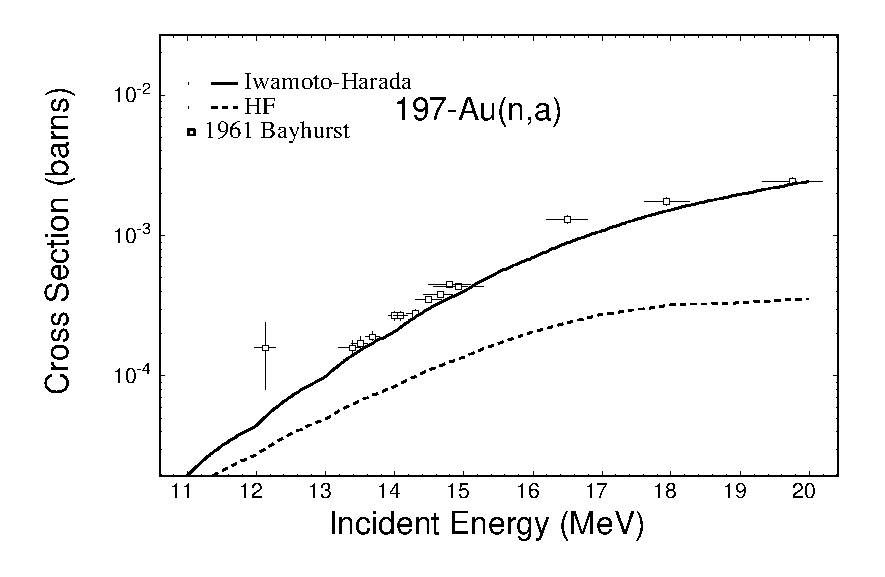
\includegraphics{hermanm1_f4.eps}}
\caption{Improvement in the description of the $^{179}$Au(n,$\protect\alpha $%
) reaction achieved by employing the Iwamoto-Harada model for preequilibrium
emission of $\protect\alpha $-particles.}
\label{goldna}
\end{figure}

\paragraph{Probability of gamma emission}

The probability of emission of gamma radiation (without spin selection
rules) is derived in a way similar to the nucleon emission probability by
applying the principle of detailed balance \cite%
{Pluyko:78,Betak:79,Akkermans:85} and can be expressed as%
\begin{eqnarray}
W_{\gamma }(E,n,\epsilon _{\gamma })&=&\frac{1}{\pi ^{2}\hbar ^{3}c^{2}}%
\epsilon _{\gamma }^{2}\sigma _{\gamma }^{inv}(\epsilon _{\gamma })\times
\notag \\
&&\frac{\sum\limits_{k}b(k\rightarrow n,\epsilon _{\gamma })\omega
_{res}(p,h,U)}{\omega _{CN}(p,h,E)}.
\end{eqnarray}%
Coefficients $b(k\rightarrow n,\epsilon _{\gamma })$ are the branching
ratios derived by Gruppelaar and Akkermans \cite{Akkermans:85}. The inverse
reaction cross section $\sigma _{\gamma }^{inv}(\epsilon _{\gamma })$ in
the gamma channel is calculated taking into account only the contribution of
the GDR.

\paragraph{Initial and equilibrium number of excitons}

Calculations in the PCROSS module start with exciton number $n=1$, thus
taking into account the direct gamma emission. The equilibrium exciton
number is taken equal to $\sqrt{1.4 gE}$ \cite{Shang:88,Shang:89}.

\bigskip

The exciton model, as implemented in the PCROSS code, has been extensively
used in recent evaluations. Combined with the direct contribution described in
terms of the CC+DWBA models, it gave an excellent description of the forward
inelastic scattering of neutrons on $^{232}$Th in the energy range from 6.1
MeV up to 18 MeV as can be seen in Fig. \ref{thspectra}.

\begin{figure}[htbp]
\scalebox{0.6}{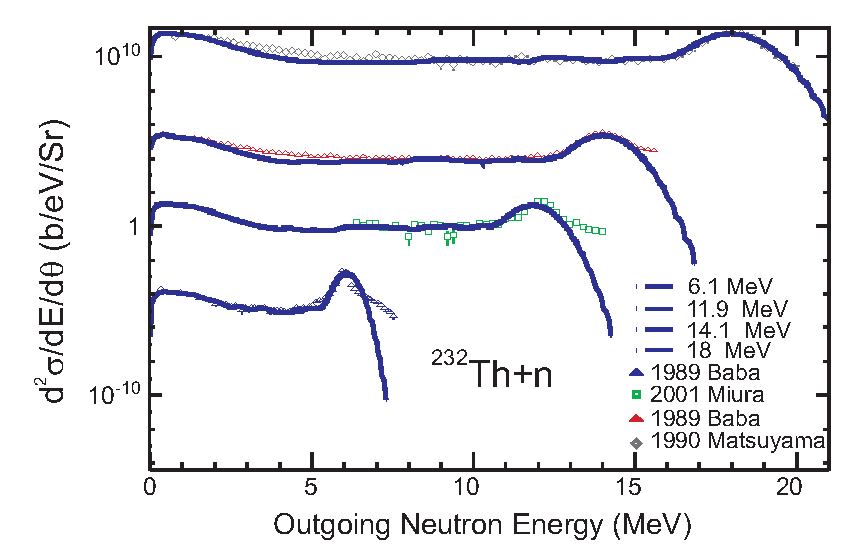
\includegraphics{thspectra.eps}}
\caption{EMPIRE calculations of the spectra of neutrons emitted at 30 degrees
for 6.1, 11.9, 14.1 and 18 MeV neutrons incident on $^{232}$Th (scaled
by 1, 10$^3$,10$^6$ and 10$^9$ respectively). Fission neutrons are not
included.}
\label{thspectra}
\end{figure}

The 18 MeV emission spectra at 60 degrees extracted from the recent IAEA
evaluation included in the ENDF/B-VII library is compared to previous
evaluations in Fig. \ref{thspectra18}. The advanced modeling resulted in a
dramatic improvement of the high energy part of the spectrum compared to the
previous evaluations.

\begin{figure}[htbp]
\scalebox{0.8}{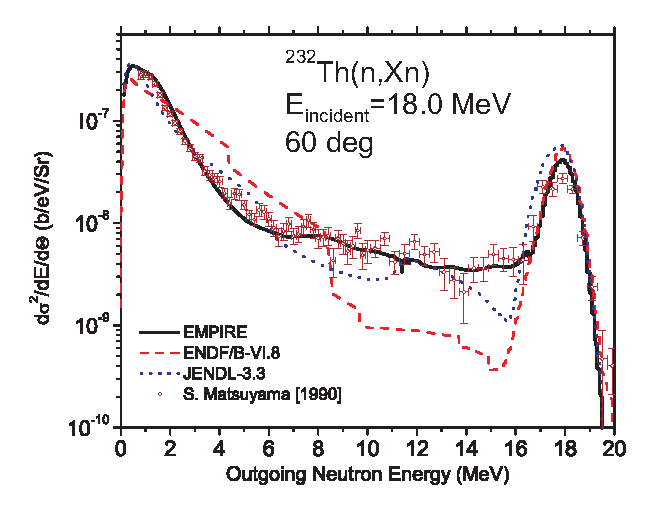
\includegraphics{thorium.eps}}
\caption{EMPIRE calculation for the neutron emission spectrum at 60 degree
for an incident neutron energy of 18.0~MeV on $^{232}$Th, compared to
experimental data~\protect\cite{mats} and the ENDF/B-VI.8 and JENDL-3.3
libraries.}
\label{thspectra18}
\end{figure}

%%%%%%%%%%%%%%%%%%%%%%%%%%%%%%%%%%%%%%%%%%%%%%%%%%%%%%%%%%%%%%%%%%%%%%%%%%%%%%%%%%%%%%%%%%%%%%%%%%%%%%%%%%%%%%%%%%

\subsubsection{Monte Carlo Preequilibrium\label{DDHMS}}

The Hybrid Monte-Carlo Simulation (HMS) approach to the preequilibrium
emission of nucleons has been formulated by M. Blann \cite{Blann-HMS} as a
hybrid model \cite{hybrid,hybrid1,hybrid2,hybrid3} inspired version of the
intranuclear cascade approach. Contrary to other classical preequilibrium
models, this approach avoids multi-exciton level densities%
\index{p-h level densities}, which were shown by Bisplinghoff \cite%
{Bisplinghoff} to be used inconsistently in the exciton and in the hybrid
formulations. The HMS%
\index{HMS} model has a number of attractive features. First of all, there
are no physical limits on the number of preequilibrium emissions (apart from
energy conservation). With the addition of linear momentum conservation by
M. Chadwick and P. Oblo\v{z}insk\'{y}
(DDHMS), the model provides a nearly complete set of observables.
These include cross sections for the production of residuals, light-particle
double-differential spectra and spectra of recoils. Spin and
excitation-energy dependent populations of residual nuclei can also be
obtained, an essential feature for coupling the preequilibrium mechanism to
the subsequent Compound Nucleus decay. The binding energies in the HMS%
\index{HMS} model are thermodynamically correct. The DDHMS model proved to
perform very well
%up to at least 250 MeV, extending energy range of the EMPIRE applicability
up to at least 250 MeV. %to the desired limit.
The calculation flow in the DDHMS model can be summarized in terms of the
following steps:

\begin{enumerate}
\item draw a collision partner for the incoming nucleon (2p-1h state created)

\item draw the energy ($\varepsilon$) of the scattered nucleon (if bound go to
step 5)

\item draw scattering angles for both particles

\item decide whether the scattered nucleon will be emitted, re-scattered or
trapped

\begin{enumerate}
\item if emitted, the appropriate cross section is augmented

\item if re-scattered, an additional particle-hole is created and one returns to
step 2

\item if trapped, go to step 5
\end{enumerate}

\item draw the excitation energy of a particle in the remaining 1p-1h
configurations (between 0$\div(U-\varepsilon)$), if unbound go to step 3, if
bound choose another existing 1p-1h pair and repeat step 5.
\end{enumerate}

\begin{figure}[htbp]
\scalebox{0.75}{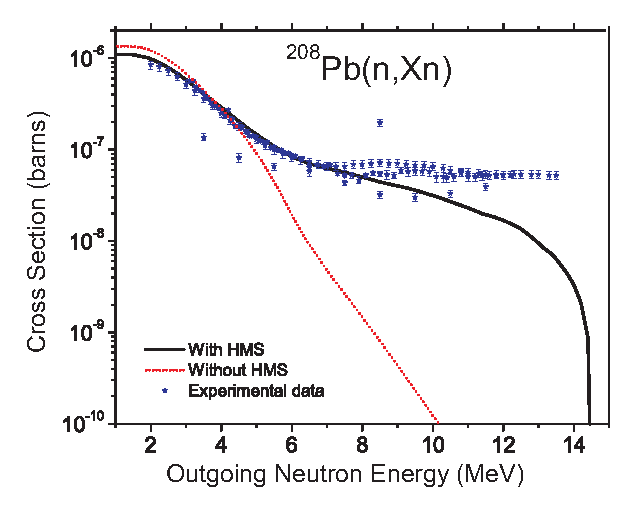
\includegraphics{pb208.eps}}
\caption{Contribution of the preequilibrium processes, modeled using Monte Carlo
simulation, to neutron spectrum from the $^{208}$Pb(n,xn) reaction at 14.6
MeV.}
\label{pb208HMS}
\end{figure}

All excitons (including holes) are treated on an equal footing and each of them
is given a chance to interact or be emitted with \emph{a priori} equal
probability. The cascade ends when all excitons are bound. Below, we
summarize various probability distributions which are used in concert with a
random number generator. For choosing a collision partner, it is assumed that
the unlike interaction is 3 times more probable than the like one ($%
\sigma_{np}=3\sigma_{nn}$). Thus, for an incident neutron we have $P_{nn}$
and $P_{np}$ for the probability of exciting neutron and proton respectively
\begin{equation}
P_{nn}=%
\frac{(A-Z)}{(A-Z)+3Z},  \label{Pnn}
\end{equation}

\begin{equation}
P_{np}=1-P_{nn}  \label{Pnp}
\end{equation}
and similarly for an incident proton
\begin{equation}
P_{pp}=\frac{Z}{Z+3(A-Z)},  \label{Ppp}
\end{equation}
\begin{equation}
P_{pn}=1-P_{pp}.  \label{Ppn}
\end{equation}
The energy distribution of the scattered particles $P(\varepsilon)$ is given
by the ratio of the $(n-1)-$ and $n$-exciton level densities%
\index{p-h level densities} $\rho_{n}$
\begin{equation}
P(\varepsilon)d\varepsilon=%
\frac{\rho_{n-1}(E-\varepsilon)g}{\rho_{n}(E)}d\varepsilon,  \label{Penergy}
\end{equation}
with $n=2\, or\,3$ and%
\begin{equation}
\rho_{2}(E)=\frac{g(gV)}{2}\,\,\, if\,\,\, E>V,  \label{ro2u}
\end{equation}
\begin{equation}
\rho_{2}(E)=\frac{g(gE)}{2}\,\,\, if\,\,\, E\leq V,  \label{ro2d}
\end{equation}
\begin{equation}
\rho_{3}(E)=\frac{g^{3}\left[V(2E-V)\right]}{4}\,\,\, if\,\,\, E\geq V.
\label{ro3}
\end{equation}
Here, $V$ is the potential well depth. The emission probability is calculated
as
\begin{equation}
P_{\nu}(\varepsilon-Q)=\frac{\lambda_{c}(\varepsilon-Q)}{\lambda_{c}(%
\varepsilon-Q)+\lambda_{+}(\varepsilon)},  \label{Pnu}
\end{equation}
with the emission rate being
\begin{equation}
\lambda_{c}(\varepsilon-Q)\sim\frac{\sigma_{\nu}(\varepsilon-Q)(%
\varepsilon-Q)(2S+1)\mu_{\nu}}{g}.  \label{lambdac}
\end{equation}
Here, $\sigma_{\nu}$ is the inverse reaction cross section, $Q$ is the binding
energy, $g$ is the single particle density, $S$ denotes nucleon spin, and $%
\mu_{\nu}$ stands for the reduced nucleon mass. Following the hybrid%
\index{HYBRID} model, $\lambda_{+}(\varepsilon)$ is calculated from the mean
free path of a nucleon in nuclear matter. The version which is actually
implemented in EMPIRE was coded by M. Chadwick and extended to
double-differential cross sections in collaboration with P. Oblo\v zinsk\' y
\cite{DDHMScode}.

Figure~\ref{pb208HMS} presents the effect of the HMS contribution on spectrum of
neutrons emitted from $^{208}$Pb bombarded with 14.6~MeV neutrons. The
compound nucleus emission underestimates
the experimental data starting at $\sim$5 MeV)
and at higher emission energies it is practically negligible. The HMS model
contribution is of the right order of magnitude to bring the
calculations into a
reasonable agreement with the measurements. One notes, however, that the
model still fall short of the experimental data above 8 MeV. This
deficiency could be counteracted by adjusting the HMS input parameters (e.g.,
single particle level densities) but such an intervention would be unphysical.
The real reason for the discrepancy is the lack of a direct reaction
contribution in the calculations reported in Fig.~\ref{pb208HMS}.

\subsubsection{Compatibility of Preequilibrium Models}

The inclusion of different preequilibrium models in a single
calculation introduces the possibility of double-counting.
The current version of
EMPIRE has 5 modules for preequilibrium decay: MSD, MSC, DEGAS and HMS and
PCROSS. While MSD and MSC describe different reaction mechanisms and are
complementary, neither of them is compatible with DEGAS, HMS or PCROSS.
Therefore, neither of the latter three should be used together with MSD or MSC
in the same exit channel. Also DEGAS, HMS and PCROSS mutually exclude each
other. However, these models can be combined if used in different exit
channels. For example, neutron inelastic scattering may be calculated using
MSD and MSC while the emission of protons can be treated within the exciton
model using PCROSS. We also note that summing $\gamma$-emission spectra from
more than one of the three possible mechanisms (MSC, DEGAS, and PCROSS)
would obviously be multiple counting and must be avoided. An additional
complication is introduced by the possibility of using ECIS03, which
calculates Coupled-Channel or DWBA contributions to the collective discrete
levels. In general, these contributions are so strong that adding those
provided by the exciton model leave the results practically unchanged. Thus,
ECIS03 can be considered compatible with HMS since the latter does not
include collective excitations. By the same token ECIS03 is not compatible
with MSD as both include collectivity of discrete levels. However, ECIS03
and MSD can be combined providing that only the continuum contribution from
the MSD is retained. To avoid double-counting when combining different
models, EMPIRE applies the following priorities:

\begin{description}
\item[ECIS03] provides inelastic scattering to collective levels
independently of the settings for the remaining models.

\item[MSD] provides inelastic continuum cross sections
independently of other settings. It
also provides vibrational inelastic excitation to discrete levels unless it is
suppressed by the active ECIS03 option. A user, at his own discretion, may
retain the MSD contribution and sum it with the results of the CC
calculations. This option might be physically acceptable for deformed nuclei
to account for both rotational (CC) and vibrational (MSD) contributions.
Note the provision for the second-chance preequilibrium emission after MSD.

\item[MSC] results are taken for the inelastic emission to the continuum.
Charge-exchange to the continuum is accepted if not suppressed by use of
DEGAS, HMS or PCROSS.

\item[PCROSS] provides inelastic and charge-exchange reactions
to the continuum if MSD
and MSC are not active. It provides $\gamma$-emission if not suppressed by $%
\gamma$-emission from MSC or DEGAS. It provides preequilibrium emission of
clusters independently of the settings for other models.

\item[DEGAS] provides inelastic and charge-exchange reactions
to the continuum if
these are not provided by any of the above listed models. Gamma emission
from DEGAS overwrites that from PCROSS and is used if not provided by the
MSC.

\item[HMS] provides inelastic and charge-exchange reactions
to the continuum and to
discrete levels if MSD and MSC are not active. Otherwise only the
charge-exchange contribution is used. DEGAS and PCROSS results
for particle emission are suppressed if they were calculated.
HMS does not calculate $\gamma$-emission.
Thus MSC, DEGAS or PCROSS results (in this order!) are adopted.
\end{description}

This scheme allows the user to activate any combination of reaction mechanisms
while the code ensures the internal consistency of calculations. Overlapping
contributions from various models are summed up and the compound nucleus
contribution is added in all cases. A concise summary explaining use of the
models is printed as a table at the beginning of the EMPIRE output. An
example is reproduced below:
\begin{verbatim}
Use of preequilibrium models
-------------------------------------------
Exit channel ECIS MSD MSC DEGAS HMS PCROSS
neut. disc.   0    1   0    0    0    0
neut. cont.   0    1   1    0    0    0
prot. disc.   0    0   0    0    0    1
prot. cont.   0    0   0    0    0    1
gammas        0    0   0    1    0    0
alpha cont.   0    0   0    0    0    1
-------------------------------------------
\end{verbatim}

\noindent 1 indicates that the contribution of the model is included, and 0
means that it is not calculated or is ignored. In the above example, MSD%
\index{MSD}, MSC%
\index{MSC}, DEGAS%
\index{DEGAS} and PCROSS%
\index{PCROSS} were invoked, and priority rules caused the PCROSS neutron
contribution to be suppressed as well as all DEGAS contributions except
emission of gammas. Selecting DIRECT =1 (or 2 or 3), MSD=1, MSC=1, PCROSS=1
is supposed to give the best results at low incident energies (say up to 30
MeV). At higher incident energies, preference should be given to the HMS%
\index{HMS} model, which accounts for multiple preequilibrium emission.
When selecting appropriate models the user should take into account that not
all of them provide the same set of observables. In particular, DEGAS%
\index{DEGAS} does not produce angular distributions,
which are calculated by
PCROSS and HMS. On the other hand, preequilibrium $\gamma$-emission can be
obtained from DEGAS, PCROSS or MSC but not from HMS. Finally, we note that
DEGAS is the only $\gamma$-emission preequilibrium model with proper angular
momentum coupling.

\subsubsection{\label{sec:photonuclear} Photo-nuclear Reactions}

A model of photo-nuclear reactions must account for the different reaction
mechanisms involved in the initial photo-nuclear excitation process and the
subsequent decay of the excited nucleus by particle and $\gamma$-ray
emission. At low energies, below about 30 MeV, the Giant Dipole Resonance
(GDR) is the dominant excitation mechanism, where a collective bulk
oscillation of the neutrons against the protons occurs. At higher energies,
up to approximately 150 MeV, photo-absorption on a neutron-proton pair (a
quasi-deuteron, QD), which has a large dipole moment, is the dominant
mechanism. In EMPIRE, the photo-absorption cross section is calculated as the
sum of the two components~\cite{PHNuc},
\begin{equation}
\sigma_{abs}(E_{\gamma})=\sigma_{GDR}(E_{\gamma})+\sigma_{QD}(E_{\gamma}).
\end{equation}
The GDR component, $\sigma_{GDR}(E_{\gamma})$, is given by a Lorentzian
shape, with parameters describing the total absorption of the giant dipole
resonance. The expression used is given in detail in 2.9.5, but takes the
basic form
\begin{equation}
\sigma_{GDR}(E_{\gamma})=\sum_{i}\sigma_{i}%
\frac{(E_{\gamma}\Gamma_{i})^{2}}{(E_{\gamma}^{2}-E_{i}^{2})^{2}+(E_{\gamma}%
\Gamma_{i})^{2}}\,,
\end{equation}
\noindent where $\sigma_{i}$, $E_{i}$ and $\Gamma_{i}$ are the GDR peak
cross section, energy and width, respectively. The summation is limited to $%
i=1$ for spherical nuclei, while for deformed nuclei the resonance is split
and one uses $i=1,2$. As a rule, the parameters are derived from fits to
experimental data or from systematics~\cite{RIPL2}. The QD component, $%
\sigma_{QD}(E_{\gamma})$, is taken from the model of Chadwick~\emph{et al.}~%
\cite{chadQD}, which uses a Levinger-type theory. It relates the nuclear
photo-absorption cross section to the experimental deuteron
photo-disintegration cross section, $\sigma_{d}(E_{\gamma})$, as
\begin{equation}
\sigma_{QD}(E_{\gamma})=L\frac{NZ}{A}\sigma_{d}(E_{\gamma})\,
f(E_{\gamma})\,.
\end{equation}
Here, the Levinger parameter was derived as $L=6.5$ and $f(E_{\gamma})$ is
the Pauli-blocking function, which reduces the free deuteron cross section $%
\sigma_{d}(E_{\gamma})$ to account for Pauli blocking of the excited neutron
and proton by the nuclear medium. The experimental deuteron
photo-disintegration cross section was parametrized as
\begin{equation}
\sigma_{d}(E_{\gamma})=61.2\frac{(E_{\gamma}-2.24)^{3/2}}{E_{\gamma}^{3}}\,,
\end{equation}
with $E_{\gamma}$ in MeV and $\sigma_{d}$ in mb. The Pauli-blocking function
was found by Chadwick \emph{et al.} to be a multidimensional integral whose
solution could be well approximated in the energy range 20 -- 140 MeV by the
polynomial expression
\begin{eqnarray}
f(E_{\gamma}) & = & \;8.3714\times10^{-2}-9.8343\times10^{-3}E_{\gamma}
\notag \\
&+&4.1222\times10^{-4}E_{\gamma}^{2} -3.4762\times10^{-6}E_{\gamma}^{3}
\notag \\
&+&9.3537\times10^{-9}E_{\gamma}^{4}\,,
\end{eqnarray}
with $E_{\gamma}$ in MeV. In Ref.~\cite{chadQD}, the Pauli-blocking function
was not parametrized below 20 MeV, where it tends to zero, or above 140 MeV,
where it tends to unity. As the contribution must be defined at all
energies considered, EMPIRE follows the example of Ref.~\cite{PHNuc} and
uses an exponential shape, $f(E_{\gamma})=\exp(-D/E_{\gamma})$, for energies
below 20 MeV and above 140 MeV, with $D=73.3$ MeV for $E_{\gamma}<20$ MeV
and $D=24.2$ MeV for $E_{\gamma}>140$ MeV. This form has the correct
behavior in that it tends to zero at $E_{\gamma}=0$ and to unity for large $%
E_{\gamma}$, and is continuous with the previous equation at 20 and 140 MeV.
Preequilibrium reaction mechanisms become important for incident photon
energies above 10 to 15 MeV. In the photo-absorption mechanisms described
above, the initial nuclear excitation can be understood in terms of
particle-hole excitations ($1p-1h$ for the GDR; $2p-2h$ or $2p-1h$ for QD
processes) and thus it is natural to use a preequilibrium theory of
particle-hole processes to describe the preequilibrium emission and damping
to equilibrium during the evolution of the reaction. Such models can be used
to calculate photo-nuclear reactions for incident photons with energies up
to about 140 MeV, which is the threshold for pion production.
\begin{figure}[htbp]
\scalebox{0.16}{\includegraphics{u235abs.eps}}
\caption{Comparison of an EMPIRE calculation and experimental data for
photo-absorption on $^{235}$U.}
\label{u235abs}
\end{figure}

At present, EMPIRE permits the calculation of preequilibrium emission in
photo-nuclear reactions using either the exciton model module PCROSS%
\index{PCROSS} or the Hybrid Monte-Carlo Simulation module HMS%
\index{HMS}. Both implementations of photo-absorption represent the GDR
fraction as an initial $1p-1h$ excitation and the QD fraction as an initial $%
2p2h$ excitation. The implementation of photo-absorption in PCROSS does not
take into account the correlation of the two holes created through the QD
mechanism, which would require an initial configuration closer to a $2p1h$
one than to a $2p-2h$ one~\cite{PHNuc}. The implementation in HMS takes this
correlation into account in a manner consistent with the model of Ref.~\cite%
{chadQD}. Following the possible emission of preequilibrium particles, the
remaining nuclear system reaches equilibrium, after which it decays by
sequential particle or gamma-ray emission (or possibly fission) until the
nuclear ground state is reached. In EMPIRE, the Hauser-Feshbach theory is
used to calculate cross sections for these processes. Much more information
on photo-nuclear reactions can be found in Ref.~\cite{PHNuc}, which served
as the basis for this brief description of these processes. For illustration
of the capability of the EMPIRE code, Fig.~\ref{u235abs} compares
calculated and experimental photo-absorption cross sections on $^{235}$U
using the ML01 $\gamma$-ray strength function~\cite{mike2}.

%%%%%%%%%%%%%%%%%%%%%%%%%%%%%%%%%%%%%%%%%%%%%%%%%%%%%%%%%%%%%%%%%%%%%%%%%%%%%%%%%%%%%%%%%%%%%%%%%%%%%%%%%%%%%%%%%%

\subsection{Compound Nucleus Reactions}

The statistical model used in the EMPIRE is an advanced implementation of
the Hauser-Feshbach theory. The exact angular momentum and parity coupling
is observed. The emission of neutrons, protons, $\alpha$-particles, and a
light ion is taken into account along with the competing fission channel.
The full $\gamma$-cascade in the residual nuclei is considered. Particular
attention is dedicated to the determination of the level densities%
\index{level densities}, which can be calculated in the non-adiabatic
approach allowing for the rotational and vibrational enhancements. These
collective effects are gradually removed above a certain energy. Level
densities acquire dynamic features through the dependence of the rotational
enhancement on the shape of the nucleus. In the frame of the statistical model
of nuclear reactions, the contribution of the Compound Nucleus (CN) state $a$
with spin $J$, parity $\pi$, and excitation energy $E$ to a channel $b$ is
given by the ratio of the channel width $\Gamma_{b}$ to the total width $%
\Gamma_{tot}=\sum_{c}\Gamma_{c}$ multiplied by the population of this state $%
\sigma_{a}(E,J,\pi)$. This also holds for secondary CNs that are formed due
to subsequent particle emission. The only difference is that while the
first CN is initially excited to the unique (incident channel compatible)
energy, the secondary CNs are created with excitation energies that spread
over the available energy interval. Each such state contributes \noindent
\begin{equation}
\sigma_{b}(E,J,\pi)=\sigma_{a}(E,J,\pi)%
\frac{\Gamma_{b}(E,J,\pi)}{\sum_{c}\Gamma_{c}(E,J,\pi)}  \label{Hauser}
\end{equation}
\noindent to the cross section. These have to be summed over spin $J$ and
parity $\pi$, and integrated over excitation energy $E$ (in the case
of a daughter
CN) to obtain observable cross sections. The particle decay width is given
by
\begin{eqnarray}
\Gamma_{c}(E,J,\pi)&=&\frac{1}{2\pi\rho_{CN}(E,J,\pi)}  \notag \\
&\times&\sum_{J^{\prime}=0}^{\infty}\sum_{\pi^{\prime}}\sum_{j=J^{%
\prime}-J}^{J+J^{\prime}}\int_{0}^{E-B_{c}}\rho_{c}(E^{\prime},J^{\prime},%
\pi^{\prime})  \notag \\
&\times&T_{c}^{l,j}(E-B_{c}-E^{\prime})dE^{\prime},  \label{pwidth}
\end{eqnarray}
\noindent where $B_{c}$ is the binding energy of particle $c$ in the
compound nucleus, $\rho$ is the level density%
\index{level density}, and $T_{c}^{l,j}(\epsilon)$ stands for the
transmission coefficient for particle $c$ having channel energy $%
\epsilon=E-B_{c}-E^{\prime}$ and orbital angular momentum $l$, which
together with the particle spin $s$ couples to the channel angular momentum $%
j$. For the discrete levels (characterized by the energy $E_{i}$, spin $%
J_{i} $, and parity $\pi_{i}$) the level density $\rho(E,J^{\prime},\pi^{%
\prime})$ reduces to $\delta(E-E_{i})\delta_{(J^{\prime},J_{i})}\delta_{(%
\pi^{\prime},\pi_{i})}$. The parity selection rules are implicit in
Eq.~(\ref{pwidth}).

\paragraph{Width Fluctuations}

To account for the correlation between incident and exit channels in elastic
scattering we use the model proposed by Hofmann, Richert, Tepel and
Weidenmueller~\cite{HRTW} (HRTW). In the case of no direct reaction
contributions, the average $S$-matrix element connecting channels $a$ and $b$
can be written as
\begin{equation}
<S>_{ab}=\delta_{ab}e^{i\varsigma_{ab}}(1-T_{a})^{1/2},  \label{Sab}
\end{equation}
\noindent where
\begin{equation}
T_{a}=1-|<S>_{aa}|^{2}  \label{Ta}
\end{equation}
is an optical model transmission coefficient. The HRTW model assumes that
the Compound Nucleus (CN) cross sections factorize and can be expressed
through a product of the channel dependent quantities $\xi$. This would be
the famous assumption of Bohr, if not for the elastic enhancement factor $%
W_{a} $, which was introduced by HRTW in order to account for the
elastic channel correlation
\begin{eqnarray}
<\sigma_{ab}^{fl}>=\xi_{a}\xi_{b}\quad a\neq b \qquad and \qquad
<\sigma_{a}^{fl}>=W_{a}\xi_{a}^{2}\,.  \label{Sig-fluc}
\end{eqnarray}
Setting
\begin{equation}
\xi_{a}=%
\frac{V_{a}}{\sqrt{\sum_{c}V_{c}}}  \label{ksi}
\end{equation}
we get for the CN cross section
\begin{equation}
\sigma_{ab}^{CN}\equiv<\sigma_{ab}^{fl}>=V_{a}V_{b}\left(\sum_{c}V_{c}%
\right)^{-1}\left[1+\delta_{ab}\left(W_{a}-1\right)\right].
\label{Sig-flucV}
\end{equation}
Taking into account conservation of the incoming flux (unitary
condition), we find the relation between $V$s, the elastic enhancement factor
 $W_{a}$ and the transmission coefficient $T_{a}$,
\begin{equation}
V_{a}=T_{a}\left[1+\frac{V_{a}}{\left(\sum_{c}V_{c}\right)}%
\left(W_{a}-1\right)\right]^{-1}.  \label{Va}
\end{equation}
This equation can be solved for $V_{a}$ by iteration, once the $W_{a}$ are
known. The current version of EMPIRE uses values of $W_{a}$ derived from the analysis
of a numerically generated sets of $S$-matrices~\cite{HHM}. The resulting
formula for the elastic enhancement factor is
\begin{equation}
W_{a}=1+2\left[1+T_{a}^{F}\right]^{-1}+87\left(\frac{T_{a}-T_{ave}}{%
\sum_{c}T_{c}}\right)^{2}\left(\frac{T_{a}}{\sum_{c}T_{c}}\right)^{5},
\label{Wa}
\end{equation}
with
\begin{equation}
F=4\frac{T_{ave}}{\sum_{c}T_{c}}\left(1+\frac{T_{a}}{\sum_{c}T_{c}}%
\right)\left(1+3\frac{T_{ave}}{\sum_{c}T_{c}}\right)^{-1},  \label{Wa-F}
\end{equation}
which completes the formulation of the model. EMPIRE uses the HRTW model
by default below 5 MeV incident energy.

\subsubsection{Photon Emission}

The E1, E2, and M1 transitions are taken into account in the statistical
model (Hauser-Feshbach%
\index{Hauser-Feshbach}) default calculations using the Giant Multipole
Resonance model known as Brink-Axel hypothesis \cite{Axel,Brink,Brinka}. The
Brink-Axel hypothesis allows the cross section for photo-absorption by an
excited state to be equated with that of the ground state. Introducing the $%
\gamma$-ray strength function $f_{Xl}(E_{\gamma})$, the transmission
coefficient can be written as
\begin{equation}
T_{Xl}^{GMR}=2\pi f_{Xl}(E_{\gamma})E_{\gamma}^{2l+1}\,.  \label{tgGMR}
\end{equation}
The Giant Dipole Resonance (GDR) shape is generally described by the sum of
two Lorenzians with energy-dependent widths. Within the standard EGLO
approach~\cite{kop01}, the $\gamma$-ray strength function is given by the
expression \noindent
\begin{eqnarray}
f_{E1}(E_{\gamma})&=&\sum_{i=1}^{2}\sigma_{i}\Gamma_{i}\left[%
\frac{E_{\gamma}\Gamma_{i}(E_{\gamma},T)}{(E_{\gamma}^{2}-E_{i}^{2})^{2}+E_{%
\gamma}^{2}\Gamma_{i}(E_{\gamma})^{2}}\right]  \notag \\
&+&\sum_{i=1}^{2}\sigma_{i}\Gamma_{i}\left[\frac{0.7\Gamma_{i}4\pi^{2}T^{2}}{%
E^{5}}\right]  \label{lorenz}
\end{eqnarray}
\noindent where $\sigma_{i}$, $\Gamma_{i}$, and $E_{i}$ are the peak cross
section, the width, and the energy of the \emph{i}-th peak of the GDR,
respectively, and
the energy-dependent width is given by
\begin{equation}
\Gamma_{i}(E_{\gamma},T)=\Gamma_{i}\frac{E_{\gamma}^{2}+4\pi T^{2}}{E_{i}^{2}%
}\,.
\end{equation}
By default, the parameters of the GDR are estimated from systematics
based on the Dietrich and Berman compilation \cite{die88}, containing 150
experimental data for nuclei ranging from mass $A=51$ up to $A=239$.

EMPIRE also includes the series of E1 $\gamma$-ray strength functions proposed
in RIPL-2 \cite{RIPL2}. We refer to the RIPL-2 TECDOC available at
www-nds.iaea.org/RIPL-2/handbook/ripl2.pdf for detailed description of these
advanced approaches. Altogether, six different shapes of the $\gamma$-ray
strength function can be selected in the EMPIRE code:

\begin{itemize}
\item EGLO: Enhanced Generalized Lorentzian~\cite{kop01}

\item MLO1, MLO2, ML03: Modified Lorentzian~\cite{plu01,plu02,plu03}

\item GFL: Generalized Fermi Liquid Model~\cite{mug01}

\item SLO: Standard Lorentzian~\cite{bri01}
\end{itemize}

Depending on the formalism chosen, the shape of $f_{Xl}(E_{\gamma})$ is
modified, especially at the low $\gamma$-emission energies that are most
responsible for the capture cross section. Capture cross sections
calculated with these different representations are presented in Fig.~\ref%
{unresolved01}.
\begin{figure}[htbp]
\scalebox{0.78}{\includegraphics{gdr.eps}}
\caption{Comparison of the capture cross section for $^{99}$Tc calculated
with different $\protect\gamma$-ray strength functions.}
\label{unresolved01}
\end{figure}

The user may increase the maximum multipolarity from the default value of 2 (E1,
M1 and E2 transitions only) up to the maximal value of 10. This change
affects the calculation of $\gamma$-transitions between states in the continuum
as well as from the continuum to discrete levels. The radiative strength
functions for higher multipole orders ($f_{EL}$, $f_{ML}$) are calculated
using the relationships between single-particle radiative strength functions
expressed in the Weisskopf form. For the electric transitions we have
\begin{equation}
f_{E(L+1)}/f_{EL} = C E_{\gamma}^2[(3+L)/(5+L)]^2,
\end{equation}
\noindent where $C=[R/(\hbar c)]^2 = 3.7*10^{-5}A^{2/3}$, if a nuclear radius $%
R=1.2 A^{2/3}$ [fm] is assumed. For the magnetic transitions, we use
\begin{equation}
f_{M(L+1)}/f_{E(L+1)} = 10[\hbar/(m c R)]^2 = 0.307 A^{-2/3}.
\end{equation}

\subsubsection{Fission}

The fission formalism implemented in EMPIRE has been continuously updated by
incorporating fundamental features of the fission process confirmed or
revealed by recent large scale experimental and theoretical studies. It
has several unique features which make the code suitable for being used both
in basic research and data evaluation for applications:

\begin{itemize}
\item It is applicable to multi-chance fission induced by light particles and
photons starting from sub-barrier excitation energies up to about 200 MeV;

\item It describes transmission through multi-humped fission barriers
parametrized analytically or defined numerically;

\item It makes use of the optical model for fission concept to account for the
fission mechanism associated with different degrees of damping of the
vibrational states;

\item It can reproduce the resonant structure of the fission cross section in
the sub-threshold region due to the coupling among the vibrational states
within the minima of the fission path;

\item It treats multi-modal fission, providing a coherent quantitative
description of the relation between the pre-scission shapes (affecting
transition state spectra) and fission fragment properties.
\end{itemize}

A few details about these capabilities are given in the next paragraphs.
Except for multi-modal fission, which is implemented only for double-humped
barrier, all features are valid for barriers with any number of humps.
The fission coefficients for $N$-humped barriers are expressed iteratively
in terms of fission coefficients for the double-humped barrier. Therefore
only the latter will be described in this paper. Further details of the general
formula can be found in \cite{Sin:07}. \newline

\medskip

 %==============================================================

\paragraph*{Fission barriers.}

%==============================================================
Unlike the majority of reaction codes, which rely on a multiple-humped fission
barrier described by independent inverted parabolas, EMPIRE has two options
to define the fission path as a function of the quadrupole deformation: (i)
parameterizing it by smoothly-joined parabolas, or (ii) describing it numerically.

(i) In the first case, the barriers associated with the discrete transition states are
parametrized as function of the quadrupole deformation by smoothly joined
parabolas,
\begin{eqnarray}
V_{i}(\beta)=E_{fi}-\frac{1}{2}\mu\hbar^{2}\omega_{i}^{2}(\beta
-\beta_{i})^{2}\quad i=1,N  \notag \\
V_{j}(\beta)=E_{fj}+\frac{1}{2}\mu\hbar^{2}\omega_{j}^{2}(\beta
-\beta_{j})^{2} \quad j=2,N,  \label{vfund0}
\end{eqnarray}
where $N$ is the number of barriers and the number of wells ($j$ runs from 2 to
$N$ because the first well, corresponding to equilibrium deformation, is not
included in the parametrization). The energies $E_{fi(j)}$ represent
the maxima
and minima of the potential and the $\beta_{i(j)}$ are the corresponding deformations.
the harmonic oscillator frequencies $\omega_{i(j)}$ define the curvature of
each parabola and $\mu$ is the inertial mass parameter, assumed to be independent
of $\beta$ and approximated by the semi-empirical expression $%
\mu\approx0.054A^{5/3}$ MeV${}^{-1}$, where $A$ is the mass number.

In the following, the barriers will be denoted with capital letters and the
wells with Roman figures.

The discrete transition states are rotational levels built on vibrational or
non-collective band-heads, characterized by a given set of quantum numbers
(angular momentum $J$, parity $\pi$ and angular momentum projection on the
nuclear symmetry axis $K$) with the excitation energies,
\begin{eqnarray}
E_{i(j)}(KJ\pi)=E_{fi(j)}+\epsilon_{i(j)}(K,\pi)+\qquad\qquad\qquad\qquad \\
+\frac{\hbar^{2}}{2I_{i(j)}}[J(J+1)-K(K+1)]\quad i=1,N; j=2,N,  \notag
\label{tsrot}
\end{eqnarray}
where the $\epsilon_{i(j)}(K,\pi)$ are the band-head energies and the $%
\hbar^{2}/2I_{i(j)}$ are the inertial parameters (the decoupling parameter
for $K=1/2$ bands was neglected). A parabolic barrier with height(depth) $%
E_{i(j)}(J,K,\pi)$ and curvature $\hbar \omega_{i(j)}$ is associated to each
transition state. Usually, these are free parameters and their values are
extracted from systematics or are obtained from the fit of the experimental
fission cross section.
\begin{figure}[htbp]
\scalebox{0.56}{\includegraphics{emp-fis-bar.eps}}
\caption{Fission barrier parametrization in the optical model for fission.}
\label{fis-bar}
\end{figure}
The transition state spectrum has a discrete component up to a certain
energy $E_{ci}$, above which it is continuous and described by the level
density functions, $\rho_{i}(EJ\pi)$, accounting for collective enhancements
specific to the nuclear shape asymmetry at each saddle point (see Sec.~\ref%
{ldsaddle}).

In the optical model for fission, the damping of the vibrational states
within the wells is simulated by introducing negative imaginary potentials, $%
iW_j $, in the corresponding deformation ranges (Fig.\ref{fis-bar}). This
causes absorption of the incoming flux in these wells ~\cite{Bjornholm:80,
Bhandari:79, Back:74}. The strengths $W_j$ are assumed to be quadratic
functions of the deformation, $\beta$, like the real part, and to be energy
dependent,
\begin{equation}
W_j(\beta)=-\alpha_j(E)[E-V_j(\beta)]\quad j=2,N.
\end{equation}
The $\alpha_j(E)$ parameters, which control the strength of the imaginary
parts of the fission potential, are chosen to fit the width of the
resonances in sub-barrier fission cross section and to be consistent with
physical values for the transmission coefficients at higher energies.

The multi-modal approach assumes Brosa's channel concept and the hypothesis
that the bifurcation points appear in the deformation region corresponding
to the second minimum~\cite{Brosa:90-multimodal}. Consequently, different
discrete and continuous spectra for the transition states at the outer
saddle are considered for each mode. This is illustrated in Fig.~\ref%
{fis-multimod} for two modes known as the super-long symmetric (SL)
and the standard asymmetric (S1) modes.

\begin{figure}[htbp]
\scalebox{0.5}{\includegraphics{emp-fis-mod.eps}}
\caption{Double-humped fission barriers used in the multi-modal
calculations. }
\label{fis-multimod}
\end{figure}

(ii) As a second option for defining the fission path,
comprehensive microscopic Hartree-Fock-Bogolyubov (HFB) calculations
\cite{Goriely:07-mass} have recently become available and provide all the
nuclear ingredients required to describe the fission path from the
equilibrium deformation up to the nuclear scission. The fission barriers,
obtained by projecting the 3-D energy surfaces along the quadrupole
deformation parameter (Fig.\ref{fis-tot-bar}), are provided in tabular form.
Specialized subroutines for smoothing, finding extrema points, interpolation
and integration have been implemented in order to use the numerically defined
barriers. This capability qualifies EMPIRE as a valuable tool for testing
global microscopic fission parameters and for using them in applications
requiring a blind description of fission for nuclei far from the stability
valley.
\begin{figure}[htbp]
\scalebox{0.25}{\includegraphics{emp-fis-tot-bar.eps}}
\caption{HFB fission barriers \protect\cite{Goriely:07-mass}. The horizontal
line indicates the neutron separation energy.}
\label{fis-tot-bar}
\end{figure}
\medskip %==============================================================

\paragraph*{Fission mechanisms.}

%==============================================================
Depending on the degree of damping of the vibrational states in the
potential minima, fission occurs either by direct transmission through the
barrier, or by re-emission into the fission channel after absorption into
the isomeric well(s) (as long as delayed fission is neglected). The
fission transmission coefficients associated with these two mechanisms
(schematically illustrated in Fig.\ref{fis-mech}) are the direct
transmission coefficient ($T_{dir}$) and the indirect ($T_{ind}$) one,
respectively, their sum representing the total fission coefficient ($T_{f}$)
\begin{equation}
T_{f}(EJ\pi)=T_{dir}(EJ\pi)+T_{ind}(EJ\pi).  \label{tf}
\end{equation}
\begin{figure}[htbp]
\scalebox{0.9}{\includegraphics{emp-fis-mech.eps}}
\caption{Illustration of the transmission mechanisms through fission
barriers: direct transmission (dashed arrows) and absorption into well(s)
followed by emission in the fission channel, shape transition(s) to class I
(II) states (full arrows) or gamma-decay (wavy arrows).}
\label{fis-mech}
\end{figure}
At very low excitation energies, where the vibrational states in the
potential wells preserve their individuality, fission proceeds entirely by
direct transmission across the barrier. In the other extreme case, i.e. for
complete damping, which holds for excitation energies close or above the
top of the barrier, the entire flux transmitted through the inner hump(s) is
absorbed into the well(s) and the fission is completely determined by the
indirect mechanism. In the intermediate case, the fission process can be
described by a smooth transition between the direct and indirect
transmissions. In the optical model for fission, this is achieved by
introducing a negative imaginary potential for the deformation range
corresponding to the absorbing wells ~\cite{Bhandari:79, Back:74}. A simpler
way to describe the degree of damping is by assigning energy-dependent
weights to the direct and indirect fission coefficients. Details about both
approaches are given in the following paragraphs.

The flux absorbed in the well(s) can: \newline
\qquad (i) be re-emitted in the fission channel by direct transmission
through the outer hump(s); \newline
\qquad (ii) be absorbed in another well (undergo a shape transitions);
\newline
\qquad (iii) undergo a $\gamma $-transition to the isomeric state. The
isomeric state, in turn, can decay by delayed (isomeric) fission or by shape
transitions.

The general expression for the indirect term is a sum of $N-1$ terms, where $%
N-1$ is the number of wells. The term $j$ represents the product of the
absorption coefficient $T_{abs_{j}}$ and the fission probability $P_{f_{j}}$
associated with the $j$-th well
\begin{equation}
T_{ind}=\sum_{j=2}^{N}T_{abs_{j}}P_{f_{j}}.  \label{tf1}
\end{equation}%
For a double-humped fission barrier, the above relation becomes

\begin{equation}
T_{ind}=T_{abs}\frac{T_{B}+RT_{\gamma_{II}}} {T_{A}+T_{B}+T_{\gamma_{II}}},
\end{equation}
where $T_{A}$ is the transmission coefficient through the first peak, $T_{B}$
is the direct transmission coefficient through the outer peak, $T_{\gamma
_{II}}$ describes gamma-decay in the isomeric well and $R$ is the branching
ratio for fission of the isomeric state. In most of the cases $T_{\gamma
_{II}}$ is small and is usually neglected.

\medskip %==============================================================

\paragraph*{Fission coefficients.}

%==============================================================
The transmission coefficients are expressed in the first-order WKB approximation
in terms of the momentum integrals for each hump~\cite{Froman:65}:
\begin{equation}
K_{i}=\pm\left\vert
\int_{a_{i}}^{b_{i}}[2\mu(E-V_{i}(\beta))/\hbar^{2}]^{1/2}d\beta\right\vert
\,,\quad i=1,N,
\end{equation}
where the $+$ sign is taken when the excitation energy is lower than the
hump under consideration and the $-$ when it is higher. In the latter case,
the intercepts are complex conjugate ( $b_{i}=a_{i}^{\ast}$) and the WKB
approximation is valid when their imaginary parts are small, \textit{i.e.},
for energies slightly higher than the hump. The single-hump transmission
coefficients, $T_{i}$, turn out to be
\begin{equation}
T_{i}=\frac{1}{1+\exp(2K_{i})}\,\quad i=1,N.  \label{single_hump}
\end{equation}
As is known, in the case of a single parabolic barrier, Eq.~(\ref%
{single_hump}) yields the well-known Hill-Wheeler transmission coefficient~%
\cite{Bjornholm:80}
\begin{equation}
T_{HW}=\frac{1}{1+\exp\left[ (2\pi/{\hbar\omega}){(V-E)}\right] }\,,
\label{HW}
\end{equation}
which is an exact result.

In the intermediate wells, where the intercepts, $a_{j}$ and $b_{j}$, are
real, the momentum integrals depending on the real parts of the potential
are approximated as:
\begin{equation}
\nu_{j}=\int_{a_{j}}^{b_{j}}[2\mu(E-V_{j}(\beta))/\hbar^{2}]^{1/2}d\beta%
\quad j=2,N.
\end{equation}

\medskip

\paragraph*{Optical model for fission.}

The direct transmission coefficient through a real double-humped fission
barrier (without absorption) reads~\cite{Bhandari:79}
\begin{equation}
T_{dir_{(0)}}=\frac{T_{A}T_{B}}{1+2B^{1/2}\cos (2\nu_{2})+B},  \label{tdir_20}
\end{equation}%
where $B=(1-T_{A})(1-T_{B})$. For barriers with more than two humps, the
transmission coefficients can be calculated iteratively, using as reference
the above equation. For example, in the case of a triple-humped barrier, in Eq.%
(\ref{tdir_20}), the direct transmission through the outer hump $T_B$ is
replaced with the direct transmission through the outer humps $T_{BC}$,
which is calculated with the same Eq.~(\ref{tdir_20}).

In the optical model for fission, the partial damping of the vibrational
states within the wells, causing the absorption of the initial flux supposed
to be emitted in the fission channel, is simulated by the imaginary
potentials introduced in the deformation ranges corresponding to the minima
of the nuclear potential. The expression for the fission coefficient
describing direct transmission through a double-humped barrier in the
presence of absorption is a generalization of Eq.~(\ref{tdir_20}). It is
obtained by adding to the real momentum integrals $\nu _{j}$ the imaginary
contributions $\delta _{j}$ corresponding to the imaginary potentials \cite%
{Bhandari:79}
\begin{equation}
\delta _{j}=-\left( \frac{\mu }{2\hbar ^{2}}\right)
^{1/2}\int_{a_{j}}^{b_{j}}\frac{W_{j}(\beta )}{[E-V_{j}(\beta )]^{1/2}}%
d\beta \,\quad j=2,N.
\end{equation}%
The direct transmission coefficient and the absorption coefficient for a
complex double-humped fission barrier read
\begin{equation}
T_{dir}=\frac{T_{A}T_{B}}{e^{2\delta _{2}}+2B^{1/2}\cos (2\nu
_{2})+Be^{-2\delta _{2}}}  \label{tdir_2}
\end{equation}%
\begin{equation}
T_{abs}=T_{dir}\frac{e^{2\delta _{2}}-(1-T_{B})e^{-2\delta _{2}}-T_{B}}{T_{B}%
}\,.  \label{tabs_2}
\end{equation}%
Further details about the iterative expressions for direct and absorption
coefficients for multi-humped fission barriers are given in \cite{Sin:07a}.

The total fission coefficient which enters the statistical model of nuclear
reactions corresponds to a well-defined spin and parity. Both direct transmission
and absorption in the isomeric well(s) occur through barriers associated
with discrete and continuous transition state spectra. Therefore, the total
fission coefficient for a given spin and parity is the sum of the
contributions of all discrete bands and continuous transition states
containing levels with these values of the spin and parity.

For the direct fission coefficient, the sum rule simply means
\begin{equation}
T_{dir}(EJ\pi)= \sum_{K\le J}T_{dir}(EKJ\pi)+ T_{dir}^{cont}(EJ\pi).
\end{equation}
The direct fission mechanism is important at low excitation energies, where
the vibrational states in the well(s) preserve their individuality.
As the excitation energy increases, the damping of the vibrational states
and the strength of the imaginary potential increase. The
entire flux transmitted through the inner hump is then absorbed in the second
(isomeric) well ($T_{abs}\rightarrow T_{A}$), and the direct transmission
through the entire barrier disappears ($T_{dir}\rightarrow0$). Therefore,
direct fission is assumed to occur only for sub-barrier excitation
energies and only through discrete channels,
\begin{equation}
T_{dir}(EJ\pi)=\sum_{K\le J}T_{dir}(EKJ\pi),  \label{tdirt}
\end{equation}
while absorption in the isomeric well occurs through all fission
channels.

For the indirect fission coefficient, the sum rule depends
on the assumptions concerning the preservation of the quantum number $K$ in
the isomeric well(s). In the description of fission cross sections, one can
consider two extreme limits: the first assumes that fission
proceeds mainly through discrete transition states characterized by well-defined
values of $K$ and is known as the "no K-mixing" approximation; the second
considers that the excitation of internal degrees of freedom in the second
well makes it possible for the nucleus to change its $K$ value during the
time the energy is bound in internal motions and is referred to
as "full K-mixing". The effect of these approximations on the fission
probability is very small, but they can affect significantly the angular
correlations of the fission fragments ~\cite{Back:74}. The appropriate
choice for the purpose of nuclear data evaluation is the "full K-mixing"
approximation, not only for physical reasons, but also because it can be
applied for any excitation energy. Formally, "full K-mixing" is described by
adding the absorption from different transition states irrespective of the
associated $K$ value to form a quantity preserving the spin and parity. The
main consequence is that the indirect fission coefficient for a certain $%
J\Pi $ is:
\begin{equation}
T_{ind}(E J \pi)=T_{abs}(E J \pi)\frac{T_{B}(E J \pi)}{T_{A}(E J
\pi)+T_{B}(E J \pi)},  \label{tind1}
\end{equation}
where $T_{\gamma_{II}}(E J \pi)$ in the denominator was neglected.

The expression for the total absorption coefficient
\begin{eqnarray}
T_{abs}(EJ\pi)=\sum_{K\le J}T_{abs}(EKJ\pi) +\qquad\qquad\quad  \notag \\
\quad\qquad + \int_{E_{cA}}^{\infty} \frac {\rho_{A}(\varepsilon
J\pi)d\varepsilon} {1+\exp\left[ -(2\pi/\hbar\omega_{A})
(E-V_{A}-\varepsilon)\right] }  \label{tabst}
\end{eqnarray}
was obtained based on the following considerations:

\begin{itemize}
\item[-] in the full $K$-mixing approximation, all discrete channels with the
same $J\pi$ contribute irrespective of their $K$ value to the total
absorption coefficient;

\item[-] the continuum fission channels contribute at higher energies, where
the class II states are completely damped and the entire flux transmitted
through the inner barrier is absorbed in the isomeric well.
\end{itemize}

Similar relations are used for the transmission coefficients through single
barriers,
\begin{eqnarray}
T_{i}(EJ\pi)=\sum_{K\le J}T_{i}(EKJ\pi) +\qquad\qquad\qquad\quad  \notag \\
+ \int_{E_{ci}}^{\infty} \frac {\rho_{i}(\varepsilon J\pi)d\varepsilon} {%
1+\exp\left[ -({2\pi}/\hbar\omega_{i}) (E-V_{i}-\varepsilon)\right] } \quad
i=A,B.  \label{tfi}
\end{eqnarray}
The general expression for the fission coefficient (Eq.~(\ref{tf})) obtained
within the optical model for fission in the "full K-mixing" approximation, valid
in any energy range, becomes
\begin{eqnarray}
T_{f}(EJ\pi)=\sum_{K\le J}T_{dir}(EKJ\pi)+\qquad\quad  \notag \\
T_{abs}(E J \pi)\frac{T_{B}(E J \pi)}{T_{A}(E J \pi)+T_{B}(E J \pi)}.
\label{tfis}
\end{eqnarray}
At very low excitation energies the strength of the imaginary potential is
very small and the only significant contribution to the total fission
coefficient comes from the direct coefficient
\begin{equation}
T_{f}(EJ\pi)=\sum_{K\le J}T_{dir}(EKJ\pi).  \label{tf-zero}
\end{equation}
For excitation energies close or above the barrier, the vibrational states
in the wells become completely damped, the direct term disappears and the
total fission coefficient (for a double-humped barrier) becomes the well
known expression
\begin{equation}
T_{f}(E J \pi)=T_{A}(E J \pi)\frac{T_{B}(E J \pi)}{T_{A}(E J \pi)+T_{B}(E J
\pi)}.  \label{tf-full}
\end{equation}
Used in almost all reaction codes, this leads to an
overestimation of the fission cross section if it is used for sub-barrier
excitation energies.

%\paragraph{Fission probabilities.}
The fission probability is usually defined as the ratio of the fission
coefficient and the sum of all the transmission coefficients (for fission
and for the competing channels $\sum_dT_d$)
\begin{equation}
P_{f}=\frac{T_{f}}{T_{f}+\sum_{d}T_{d}}.  \label{pf0}
\end{equation}
Similar definitions apply for all decay probabilities. More complicated
relations are obtained if, according to \cite{Back:74}, the coupling of
class I and class II states is considered by multiplying $T_{abs}$ with the
following weight function:%
\begin{equation}
f(x,\Gamma_{c_{II}},D_{II})=\frac{\sinh(2\pi\Gamma_{cII}/D_{II})}{\cosh
(2\pi\Gamma_{cII}/D_{II})-\cos(2\pi x/D_{II})}
\end{equation}
where $x=E-E_{0}$ is the difference between the excitation energy and the
centroid excitation energy of the class II level, $D_{II}$ is the distance
between the class II levels in the picket fence approximation, and$\ \Gamma
_{cII}$ represents the decay widths of the class II levels expressed in
terms of the transmission coefficients through the humps and for gamma decay
in the second well:\ $2\pi\Gamma_{cII}/D_{II}=T_{A}+T_{BC}+T_{\gamma II}.$
Averaging over a class II resonance, the following expressions for the decay
probabilities for fission and for the competing processes are obtained,
\begin{equation}
P_{f}=P_{dir}+P_{ind}=\frac{T_{dir}}{T_{dir}+\sum_{d}T_{d}}\left( 1-\frac {1%
}{a}\right) +\frac{1}{a}  \label{pf11}
\end{equation}
and
\begin{equation}
P_{d}=\frac{T_{d}}{T_{dir}+\sum_{d}T_{d}}\left( 1-\frac{1}{a}\right)\,,
\label{pd}
\end{equation}
where
\begin{equation}
a=\left[ 1+b^{2}+2b\coth\left( \frac{T_{A}+T_{B}+T_{\gamma II}}{2}\right) %
\right] ^{1/2},  \label{a11}
\end{equation}
and
\begin{equation}
b=\frac{(T_{dir}+\sum_{d}T_{d})(T_{A}+T_{B}+T_{\gamma II})}{%
T_{abs}(T_{B}+T_{\gamma II})}.  \label{b11}
\end{equation}

The difference between the fission cross sections obtained with Eq.~(\ref{pf0})
and Eq.~(\ref{pf11}) appears only at very low excitation energies and depends
on the parameters of the fission barrier. For more than two humps, it is
practically impossible to apply the same procedure and only the fission
probabilities given by Eq.~(\ref{pf0}) can be used.

A significant difference appears between calculations considering partial
damping (fission coefficient given by Eq.~(\ref{tfis})) and full damping
(fission coefficient given by Eq.~(\ref{tf-full})) of the vibrational states
within well(s). This is illustrated in Fig.~\ref{fis-u38-fcom} in case
of the
neutron-induced fission cross section of $^{238}$U. By assuming complete
damping for sub-barrier excitation energies, the fission cross section is
overestimated and its resonance structure is not reproduced.
\begin{figure}[htbp]
\scalebox{0.55}{\includegraphics{emp-fis-u38-fcom.eps}} .
\caption{The neutron induced fission cross section of $^{238}$U calculated with
the same set of barrier parameters but with different assumptions about the
damping of the class II vibrational states: partial damping (full curve),
complete damping (dashed curve)}
\label{fis-u38-fcom}
\end{figure}

The optical model for fission provides a realistic description of the
fission cross section, including the resonance structure at sub-barrier
excitation energies resulting from the coupling among discrete vibrational
states in different wells. Therefore, this model is recommended when a
highly
accurate description of the experimental data is required. As mentioned before,
in such cases, the parameters of the fission barriers associated with the
transition states are considered free parameters and their values are
extracted from systematics or from the fit of the experimental data. Even if
the predictive power of the model is limited, its descriptive power is
impressive (see $^{232}$Th and $^{231,233}$Pa in ENDF/B-VII.0\cite{ENDF-VII}%
).

\medskip %&&&&&&&&&&&&&&&&&&&&&&&&&&&&&&&&&&&&&&&&&&&&&&&&&&&&&

\paragraph*{Surrogate optical model for fission.}

%&&&&&&&&&&&&&&&&&&&&&&&&&&&&&&&&&&&&&&&&&&&&&&&&&&&&&
In most cases, no information is available about the barrier
parameters associated with the discrete transition states. The
transition state spectra can then be considered to be continuous and
can be described
by level densities. Analyzing the expressions of the fission coefficients in
the previous paragraph, it can be easily noticed that the coupling among the
vibrational states in the wells, determined by the degree of their damping,
is contained only in the discrete terms. By eliminating them, the general
expression for the fission coefficient reduces to Eq.~(\ref{tf-full}) which
corresponds to full damping, or in other words, to decoupled transmissions
through independent barriers (Fig.\ref{fis-ld0.eps}.a). Using this expression
would overestimate the fission cross section of fertile nuclei at low energies.
To overcome this difficulty, an alternative way of
accounting for partial damping that does not involve an imaginary potential
or discrete transition states  has been implemented in EMPIRE.
In this surrogate of the optical model for
fission, the degree of damping is taken into account by defining the total
fission coefficient as a weighted sum of the direct coefficient
corresponding to zero-damping and the indirect coefficient corresponding to
the full damping
\begin{equation}
T_{f}(EJ\pi )=(1-w(E))T_{dir_{(0)}}^{cont}(EJ\pi
)+w(E)T_{ind_{(f)}}^{cont}(EJ\pi ).  \label{tfsurr}
\end{equation}%
The term $T_{dir_{(0)}}^{cont}$ describes the direct transmission without
absorption through barriers associated to transition states in the continuum. In
order to calculate it, a level density describing the entire fission barrier
would be needed (Fig.\ref{fis-ld0.eps}.b). The problem is that the
phenomenological or microscopic models provide the level densities of the
transition states only for the maxima and minima of the fission barrier.
Assuming that the direct transmission is controlled by the minimum level
density at the saddles, the direct fission coefficient is calculated as
\begin{equation}
T_{dir}^{cont}(EJ\pi )=\int_{0}^{\infty }T_{dir_{(0)}}(\varepsilon J\pi
)\rho _{min}(\varepsilon J\pi )d\varepsilon\,,
\end{equation}%
where $T_{dir_{(0)}}$ is given by Eq.~(\ref{tdir_20}). The indirect coefficient
$T_{ind_{(f)}}^{cont}$ is calculated with Eq.~(\ref{tf-full}), where $T_{A}$
and $T_{B}$ are given by the second term in Eq.~(\ref{tfi}). The weight $w$ is
energy-dependent and ranges from 0 for excitation energies close to the
bottom of the well(s) to 1 for excitation energies close to the height of
the lowest barrier \cite{Sin:07}.
\begin{figure}[tbph]
\scalebox{0.6}{\includegraphics{emp-fis-ld0.eps}}
\caption{Illustration of the transmission mechanisms through fission
barriers: (a) decoupled transmissions through independent humps, (b) direct
transmission at low energies (dashed arrow) and decoupled transmissions at
energies comparable or higher than the barrier height (full arrows).}
\label{fis-ld0.eps}
\end{figure}
Compared to the optical model for fission, this alternative approach has the
advantage of describing the direct and indirect fission mechanisms without
involving many parameters. It can also be used when discrete transition
states are considered, but the resonant structure is not equally well
reproduced. In the optical model for fission, the imaginary potential
strength increases with increasing energy and the resonances are damped
(become wider and flatter until they disappear). In the surrogate approach
the resonances, due to the direct term, remain undamped. Only their
contribution diminishes along with the increase of the weight $w$.

This model is recommended when only the fundamental barrier and the level
densities at saddles are available. The model was used~\cite{Sin:07} to test
fission barriers obtained in microscopic calculations. A relevant
example is presented in Fig.\ref{am41-surr}.
\begin{figure}[htbp]
\scalebox{0.55}{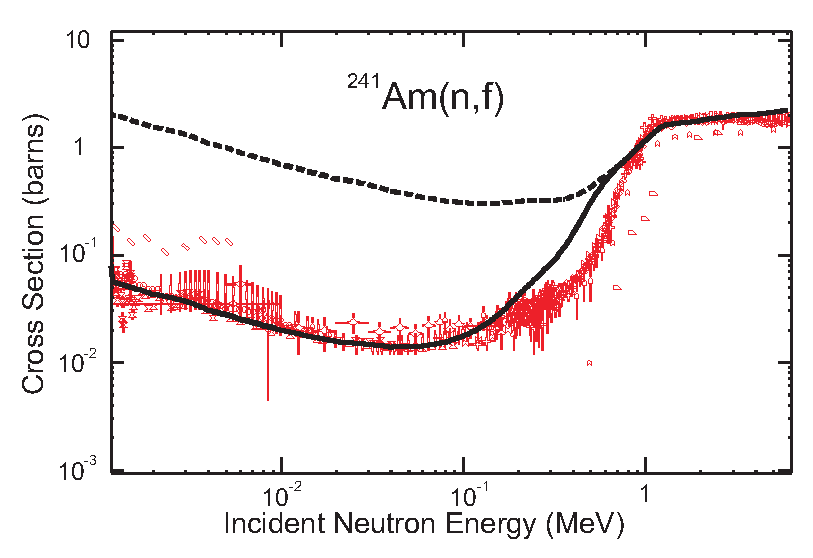
\includegraphics{emp-am41-surr.eps}}
\caption{Neutron induced fission cross sections on $^{241}$Am calculated
with microscopic fission barrier \protect\cite{Goriely:07-mass} and level
densities at the saddles \protect\cite{Goriely:07-ld}. The full curve was
obtained using Eq.~(\protect\ref{tfsurr}) and dashed curve was obtained using
Eq.~(\protect\ref{tf-full}).}
\label{am41-surr}
\end{figure}

\medskip %&&&&&&&&&&&&&&&&&&&&&&&&&&&&&&&&&&&&&&&&&&&&&&&&

\paragraph*{Multi-modal fission.}

%&&&&&&&&&&&&&&&&&&&&&&&&&&&&&&&&&&&&&&&&&&&&&&&&
The most general expressions used in EMPIRE for the fission probability
calculation were derived extending the procedure of Back~\cite{Back:74} for
multi-modal fission. For a particular mode ($m$), the decay probabilities
for direct ($P_{dir}$), indirect ($P_{ind}$), and delayed ($P_{iso}$)
fission read (the dependence on $EJ\pi$ is implicit)
\begin{equation}
P_{dir,m}=\frac{T_{dir,m}}{\sum_{m}T_{dir,m}+\sum_{d}T_{d}}\left(1-\frac{1}{a%
}\right)
\end{equation}
\begin{equation}
P_{ind,m}=\frac{T_{B,m}}{\sum_{m}T_{B,m}+T_{\gamma_{II}}}\frac{1}{a}
\end{equation}
and
\begin{equation}
P_{iso,m}=\frac{R_{f,m}^{iso}T_{\gamma_{II}}}{\sum_{m}T_{B,m}+T_{\gamma_{II}}%
}\cdot\frac{1}{a}.
\end{equation}
In order to preserve unitarity the decay probability for competing channels (%
$P_{d}$) takes the form
\begin{equation}
P_{d}=\frac{T_{d}}{\sum_{m}T_{dir,m}+\sum_{d}T_{d}}\left(1-\frac{1}{a}\right)
\end{equation}
\noindent where
\begin{equation*}
a=\left[1+b^{2}+2b\coth\left(\frac{T_{A}+\sum_{m}T_{B,m}+T_{\gamma_{II}}}{2}%
\right)\right]^{1/2}
\end{equation*}
and
\begin{equation*}
b=\frac{(\sum_{m}T_{dir,m}+\sum_{d}T_{d})(T_{A}+\sum_{m}T_{B,m})}{%
T_{abs}(\sum_{m}T_{B,m}+T_{\gamma_{II}})}.
\end{equation*}
$T_{\gamma_{II}}$ represents the $\gamma$-decay transmission coefficient in the
isomeric well and $R_{f}^{iso}$ is the branching ratio for fission of the
isomeric state. In the present version of the code, $T_{\gamma_{II}}$ and,
consequently, isomeric%
\index{isomeric fission} fission are considered negligible and are not
calculated. The fission probability for mode $m$ reads
\begin{equation}
P_{f,m}=P_{dir,m}+P_{ind,m}+P_{iso,m}
\end{equation}
and the total fission probability is obtained by summing over all modes:
\begin{equation}
P_{f}=\sum_{m}P_{f,m}
\end{equation}
At above-barrier energies, the class II vibrational states become completely
damped, the entire flux penetrating the inner barrier is absorbed in the
isomeric well ($T_{abs}\rightarrow T_{A}$), the direct transmission
disappears ($T_{dir}\rightarrow0$), the population probability of the
isomeric%
\index{isomeric} state becomes negligible ($T_{\gamma_{II}}\rightarrow0$)
and the decay widths of the class II state exceed the distance between them (%
$%
\coth[(T_{A}+\sum_{m}T_{B,m}+T_{\gamma_{II}})/2]\rightarrow1$). Under these
conditions, the fission probability becomes
\begin{equation}
P_{f,m}=\frac{T_{B,m}}{\sum_{m}T_{B,m}}\cdot\frac{1}{1+b}=W_{m}\cdot\frac{%
T_{f}}{T_{f}+\sum_{d}T_{d}}  \label{wm}
\end{equation}
\noindent where $W_{m}$ is the mode weight ($W_{m}=T_{B,m}/\sum_{m}T_{B,m}$)
and $T_{f}$ is the total fission coefficient
\begin{equation}
T_{f}=\frac{T_{A}\sum_{m}T_{B,m}}{T_{A}+\sum_{m}T_{B,m}}.
\end{equation}

%
% %%%%%%%%%%%%%%%%%%%%%%%%%%%%%%%%%%%%%%%%%%%%%%%%%%%%%%%%%%%%%%%%%%%%%%%%%%%%%%%%%%%%%%%%%%%%%%%%%%%%%%%%%%%%%%%%%%
% \subsubsection{Fission}
%
% The relation used in the statistical model for the fission cross section
% calculation is
% \begin{equation}
% \sigma_{a,f}(E)=\sum_{J\pi}\sigma_{a}(EJ\pi)P_{f}(EJ\pi),
% \end{equation}
% \noindent where $\sigma_{a}(EJ\pi)$ is the population of the fissioning nucleus
% in the state $EJ\pi$ and $P_{f}(EJ\pi)$ represents the fission probability.
% Depending on the type of particle which induces fission, EMPIRE
% offers two formalisms (selected by the directive input FISSHI) to
% calculate fission probability . The default value (FISSHI = 0) selects
% the optical model for fission (or its simplified version) to calculate
% fission induced by light particles or photons, FISSHI = 1 selects
% the Sierk model adequate for heavy ion induced fission, and FISSHI
% = 2 turns off any fission calculation.
% The default option (FISSHI = 0)  describes transmission through single-,
% double- and triple-humped fission barriers starting from sub-barrier
% excitation energies up to about 200 MeV. For multi-humped barrier,
% an expression for the fission probability is derived in the frame
% of the optical model for fission. In case of double-humped barrier,
% the expression is generalized for the case of multi-modal fission.
% For light actinides, a triple-humped fission barrier with a shallow
% tertiary well, which accommodates undamped vibrational states can
% be employed. This fission model can provide good description of experimental
% data (including gross vibrational resonant structure at sub-barrier
% energies), reasonably good predictive power and improved methodology
% for determination of fission barrier parameters.
%
% \paragraph{Fission barriers}
% The optical model for fission considers the possible transmission
% mechanisms using a complex potential ($V_{f}=V+iW$) to describe the
% uni-dimensional multi-humped fission barrier (Figures~\ref{cap:Double-humped-fission-barriers}
% , \ref{cap:Triple-humped-fission-barriers}).
% %
% \begin{figure}[htbp]
% \scalebox{0.65}{\includegraphics{emp-2bar1.eps}}
% \caption{\label{cap:Double-humped-fission-barriers}Double-humped fission
% barriers}
% \end{figure}
% %
% \begin{figure}[htbp]
% \scalebox{0.65}{\includegraphics{emp-3bar1.eps}}
% \caption{\label{cap:Triple-humped-fission-barriers}Triple-humped fission
% barriers}
% \end{figure}
% The real part of the barriers, associated with the discrete transition
% states, are parameterized as a function of the quadrupole deformation
% using smoothly joined parabolas
% \begin{equation}
% V_{i}(\beta)=E_{fi}+(-1)^{i}\frac{1}{2}\mu\hbar^{2}\omega_{i}^{2}(\beta-\beta_{i})^{2},
% \label{vfund0}
% \end{equation}
% \noindent where $i=1$ for a single barrier, runs from 1 to 3 for a two-humped
% barrier, and from 1 to 5 for a three-humped one. The energies $E_{fi}$
% represent maxima of $V_{i}$ in odd regions (humps) and minima in
% Triple-humped-fission-barriers the seven regions (wells), $\beta_{i}$ are the corresponding abscissae,
% the harmonic oscillator frequencies $\omega_{i}$ define the curvature
% of each parabola and $\mu$ is the inertial mass parameter, assumed
% independent of $\beta$ and approximated by the semi-empirical expression
% $\mu\approx0.054A^{5/3}MeV^{-1}$, where $A$ is the mass number.
% The discrete transition states are rotational levels built on vibrational
% or non-collective band-heads, characterized by a given set of quantum
% numbers (angular momentum $J$, parity $\pi$ and angular momentum
% projection on the nuclear symmetry axis $K$) with excitation energies
% \begin{equation}
% E_{i}(J,K,\pi)=E_{fi}+\epsilon_{i}(K,\pi)+\frac{\hbar^{2}}{2I_{i}}[J(J+1)-K(K+1)],
% \label{tsrot}
% \end{equation}
% \noindent where $\epsilon_{i}(K,\pi)$ are the excitation energies of the band-heads,
% and $\hbar^{2}/2I$ are inertial parameters (the Coriolis term for
% $K=1/2$ is neglected). To each transition state associated is a parabolic
% barrier with the height $E_{i}(J,K,\pi)$ and the curvature $\hbar\omega_{i}$.
% The transition state spectrum consists of a discrete part below a
% certain energy $E_{ci}$ and a continuum described by the level density
% functions $\rho_{i}(EJ\pi)$.
% Assuming Brosa's channel concept and the hypothesis that the bifurcation
% points appear in the deformation region corresponding to the second
% minimum~\cite{Brosa:90}, different discrete and continuous spectra
% for the transition states at the outer saddle are considered for each
% mode. This is illustrated in Figure \ref{cap:Double-humped-fission-barriers-multimodal}
% for two modes known as super-long symmetric (SL) and standard asymmetric
% (S1).
% %
% \begin{figure}[htbp]
% \scalebox{0.65}{\includegraphics{emp-mod1.eps}}
% \caption{\label{cap:Double-humped-fission-barriers-multimodal}Double-humped
% fission barriers used in multi-modal calculations}
% \end{figure}
% For the case of a triple-humped barrier, it is reasonable to assume
% that with increasing excitation energy the shell effects, which cause
% splitting of the outer hump, decrease and the outer humps lump into
% a single one. Therefore, in the present formalism the triple-humped
% barriers are only associated with the discrete transition states.
% Accordingly, the continuum contribution to the fission coefficient
% is calculated considering a double-humped barrier with the second
% peak representing a single barrier equivalent to the two outer humps
% (Figure~\ref{cap:Triple-humped-fission-barriers}). The parameters of the equivalent barrier
% are determined by imposing equal transmission.
% The negative imaginary potential $iW$ is introduced in the deformation
% range corresponding to the second well for both double- and triple-humped
% barriers to simulate damping of the class II vibrational states, hence,
% the absorption of the incoming flux in this well~\cite{Back:74,Bhandari:79,Bjornholm:80}.
% For the triple-humped barrier the tertiary well is supposed to be
% shallow enough to neglect damping of class III vibrational states.
% The strength $W$ depends quadratically on deformation and increases
% with the excitation energy
% \begin{equation}
% W(\beta)=-\alpha[E-V(\beta)]
% \end{equation}
%  The input parameter $\alpha$, which controls the strength of the
% imaginary part of the fission potential, should be chosen to fit the
% width of the resonances in sub-barrier fission cross section and to
% be consistent with physical values for the transmission coefficients
% at higher energies.
% In the following sections we shall denote humps with capital letters
% A,B,C (i=1,3,5) and wells with Roman figures II (i=2) and III (i=4).
%
% \paragraph{Transmission mechanisms}
% Figure~\ref{cap:Transmission-mechanisms-through-double} shows the
% transmission mechanisms through a double-humped fission barrier for
% excitation energies below both humps and above at least one of them.
% The incoming flux can be transmitted directly through the barrier
% or can be absorbed in the isomeric well. The fraction absorbed in
% the isomeric well can: (i) be re-emitted in the fission channel (indirect
% prompt fission), (ii) return back to a class I state or (iii) undergo
% $\gamma$-transition to the isomeric state. The isomeric state, in
% turn, can decay by delayed (isomeric) fission\index{isomeric fission}
% or by shape transition to class I states.
% %
% \begin{figure}[htbp]
% \scalebox{0.7}{\includegraphics{emp-2mec1.eps}}
% \caption{\label{cap:Transmission-mechanisms-through-double}Transmission mechanisms
% through a double-humped fission barrier}
% \end{figure}
% %
% \begin{figure}[htbp]
% \scalebox{0.7}{\includegraphics{emp-3mec1.eps}}
% \caption{\label{cap:Transmission-mechanisms-through-triple}Transmission mechanisms
% through a triple-humped fission barrier}
% \end{figure}
% Similar transmission mechanisms are encountered in the case of the
% triple-humped barrier (Figure~\ref{cap:Transmission-mechanisms-through-triple}),
% the main difference consisting in replacing the transmission through
% a single outer hump by the direct transmission trough the second and
% third hump. The transmission coefficients through the humps ($T_{A}$,
% $T_{B}$, $T_{C}$), for direct transmission ($T_{dir}$, $T_{BC}$)
% and absorption in the isomeric\index{isomeric fission} well ($T_{abs}$)
% are calculated in WKB approximation for complex potentials~\cite{Back:74,Bhandari:79,Ventura-3hump}.
% In the simplest version of the model (FISOPT=0), the transmission
% coefficients through the humps ($T_{A}$, $T_{B}$, $T_{C}$) of a
% barrier corresponding to a particular discrete transition state, are
% calculated with Hill-Wheeler formula
% \begin{equation}
% T_{ij}(EKJ\pi)=\frac{1}{1+\exp\{-(2\pi/\hbar\omega_{i})[E-E_{i}]\}}\quad i=A,B,C.
% \label{thw}
% \end{equation}
%  The total transmission coefficient through a hump is sum of two contributions
% corresponding to the discrete and continuous part of the transition
% state spectrum
% \begin{eqnarray}
% T_{i}(EJ\pi)&=&\sum_{K\leq J}T_{i}(EKJ\pi)\\
% &+&\int_{E_{ci}}^{\infty}\frac{\rho_{i}(\varepsilon J\pi)d\varepsilon}{{1+\exp\left[-\frac{2\pi}{\hbar\omega_{i}}(E-V_{i}-\varepsilon)\right]}\quad i}=A,B\nonumber
% \label{tjt}
% \end{eqnarray}
%  Increasing the excitation energy, the strength of the imaginary potential
% increases and the entire flux transmitted through the inner hump is
% absorbed in the second (isomeric) well ($T_{abs}\rightarrow T_{A}$),
% and the direct transmission through the entire barrier disappears
% ($T_{dir}\rightarrow0$). Therefore, the direct fission occurs only
% for sub-barrier excitation energies and occurs only through discrete
% channels
% \begin{equation}
% T_{dir}(EJ\pi)=\sum_{K\leq J}T_{dir}(EKJ\pi),
% \label{tdirt}
% \end{equation}
%  while the absorption in the isomeric well occurs through all fission
% channels. In full $K$-mixing approximation all the discrete channels
% with the same $J\pi$ contribute irrespective of their $K$ value
% to the total absorption coefficient. The continuum fission channels
% contribute at higher energies, where the class II states are completely
% damped and the entire flux transmitted through the inner barrier is
% absorbed in the isomeric\index{isomeric fission} well
% \begin{eqnarray}
% T_{abs}(EJ\pi)&=&\sum_{K\leq J}T_{abs}(EKJ\pi)\\
% &+&\int_{E_{cA}}^{\infty}\frac{\rho_{A}(\varepsilon J\pi)d\varepsilon}{{1+\exp\left[-\frac{2\pi}{\hbar\omega_{A}}(E-V_{A}-\varepsilon)\right]}}\nonumber
% \label{tabst}
% \end{eqnarray}
%  In the case of the triple-humped barrier, the total direct transmission
% through the outer humps is the sum of the transmissions through discrete
% barriers and the continuum built above the equivalent barrier
% \begin{eqnarray}
% T_{BC}(EJ\pi)&=&\sum_{K\leq J}T_{BC}(EKJ\pi)\\
% &+&\int_{E_{ceq}}^{\infty}\frac{\rho_{eq}(\varepsilon J\pi)d\varepsilon}{{1+\exp\left[-\frac{2\pi}{\hbar\omega_{eq}}(E-V_{eq}-\varepsilon)\right]}}\nonumber
% \label{tdir23t}
% \end{eqnarray}
%
% \paragraph{Decay probabilities: Double-humped barrier, multi-modal fission}
% The most general expressions used in EMPIRE for the fission probability
% calculation were derived extending the procedure of Back~\cite{Back:74}
% for multi-modal fission. For a particular mode ($m$), the decay probabilities
% for direct ($P_{dir}$), indirect ($P_{ind}$), and delayed ($P_{iso}$)
% fission read (the dependence on $EJ\pi$ is implicit)
% \begin{equation}
% P_{dir,m}=\frac{T_{dir,m}}{\sum_{m}T_{dir,m}+\sum_{d}T_{d}}\left(1-\frac{1}{a}\right)
% \end{equation}
% \begin{equation}
% P_{ind,m}=\frac{T_{B,m}}{\sum_{m}T_{B,m}+T_{\gamma_{II}}}\cdot\frac{1}{a}
% \end{equation}
% \begin{equation}
% P_{iso,m}=\frac{R_{f,m}^{iso}T_{\gamma_{II}}}{\sum_{m}T_{B,m}+T_{\gamma_{II}}}\cdot\frac{1}{a}
% \end{equation}
%  In order to preserve unitarity the decay probability for competing
% channels ($P_{d}$) takes the form
% \begin{equation}
% P_{d}=\frac{T_{d}}{\sum_{m}T_{dir,m}+\sum_{d}T_{d}}\left(1-\frac{1}{a}\right)
% \end{equation}
% \noindent where: \[
% a=\left[1+b^{2}+2b\coth\left(\frac{T_{A}+\sum_{m}T_{B,m}+T_{\gamma_{II}}}{2}\right)\right]^{1/2}\]
%  \[
% b=\frac{(\sum_{m}T_{dir,m}+\sum_{d}T_{d})(T_{A}+\sum_{m}T_{B,m})}{T_{abs}(\sum_{m}T_{B,m}+T_{\gamma_{II}})}\]
%  $T_{\gamma_{II}}$ represents $\gamma$-decay transmission coefficient
% in the isomeric well and $R_{f}^{iso}$ is the branching ratio for
% fission of the isomeric state. In the present version of the code,
% $T_{\gamma_{II}}$ and consequently the isomeric\index{isomeric fission}
% fission are considered negligible and are not calculated. The fission
% probability for mode $m$ reads
% \begin{equation}
% P_{f,m}=P_{dir,m}+P_{ind,m}+P_{iso,m}
% \end{equation}
%  and the total fission probability is obtained by summing over all
% modes:
% \begin{equation}
% P_{f}=\sum_{m}P_{f,m}
% \end{equation}
%  At over-barrier energies the class II vibrational states become completely
% damped, the entire flux penetrating the inner barrier is absorbed
% in the isomeric well ($T_{abs}\rightarrow T_{A}$), the direct transmission
% disappears ($T_{dir}\rightarrow0$), the population probability of
% the isomeric\index{isomeric} state becomes negligible ($T_{\gamma_{II}}\rightarrow0$)
% and the decay widths of the class II state exceed the distance between
% them ($\coth[(T_{A}+\sum_{m}T_{B,m}+T_{\gamma_{II}})/2]\rightarrow1$).
% In these conditions, the fission probability becomes
% \begin{equation}
% P_{f,m}=\frac{T_{B,m}}{\sum_{m}T_{B,m}}\cdot\frac{1}{1+b}=W_{m}\cdot\frac{T_{f}}{T_{f}+\sum_{d}T_{d}}
% \label{wm}
% \end{equation}
% \noindent where $W_{m}$ is the mode weight ($W_{m}=T_{B,m}/\sum_{m}T_{B,m}$)
% and $T_{f}$ is the total fission coefficient
% \begin{equation}
% T_{f}=\frac{T_{A}\sum_{m}T_{B,m}}{T_{A}+\sum_{m}T_{B,m}}
% \end{equation}
%  The decay probability through a competitive channel $d$ recovers
% the well-known form
% \begin{equation}
% P_{d}=\frac{T_{d}}{T_{f}+\sum_{d}T_{d}}
% \end{equation}
%
% \paragraph{Decay probabilities: Triple-humped barrier, single-mode fission}
% In the case of a triple-humped fission barrier with a shallow tertiary
% well, accommodating undamped vibrational states, the fission probability
% is given by the previous formulae (particularized for single-mode
% fission) where the transmission coefficient through the outer hump
% $T_{B}$ is replaced by the direct transmission coefficients through
% the outer humps $T_{BC}$.
%
%
% The fission subroutine FISFIS can be invoked by EMPIRE in two
% ways:
% \begin{itemize}
% \item default option: corresponds to the simplified version
% of the model and requires the minimum fission input. It's the only
% possible option for the single-humped barrier and is recommended for
% multi-humped barrier at over-barrier excitation energies for all fissioning
% nuclei or for odd-odd fissioning nuclei for the entire energy range.
% It considers the humps of the fission barrier to be completely decoupled
% and approximated by independent parabolas (Figure \ref{cap:Fission-barrier-parametrization-0}),
% therefore no information about the wells and the imaginary potential
% are needed. The fission probability is given by
% \begin{equation}
% P_{f}=\frac{T_{f}}{T_{f}+\sum_{d}T_{d}}
% \end{equation}
%  with\\
% \begin{tabular}{ll}
%  $T_{f}=T_{A}$&
%  single-humped barrier\tabularnewline
%  $T_{f}=\frac{T_{A}T_{B}}{(T_{A}+T_{B})}$&
%  double-humped barrier\tabularnewline
%  $T_{f}=\frac{T_{A}T_{B}T_{C}}{(T_{A}+T_{B}T_{C})}$&
%  triple-humped barrier \tabularnewline
% \end{tabular}
% \item alternative option: it selects the optical model for fission which may be applied
% for the multi-humped barriers at any excitation energy, but requires
% complete information about the complex fission potential.  This option
% is recommended for multi-humped barriers at excitation energies lower
% or around their heights, especially for even-even fissioning nuclei,
% but can not be used for single barriers. The fission coefficients
% and the decay probabilities for fission and for the competitive channels
% are calculated using the formulae presented in the previous section.
% \end{itemize}
% %
% \begin{figure}[top]
% \scalebox{0.65}{\includegraphics{emp-2ba01.eps}}
% \caption{\label{cap:Fission-barrier-parametrization-0}Fission barrier parametrization
% and transmission mechanisms corresponding to FISOPT = 0 option}
% \end{figure}
% The fission input parameters can be automatically retrieved from the
% built-in systematics and/or libraries, or can be provided by the user.
% For example, the parameters of the fundamental fission barrier are
% chosen by EMPIRE following three possibilities:
% \begin{itemize}
% \item default option: the heights of the fission barrier calculated
% within the Extended Thomas-Fermi plus Strutinsky Integral (ETFSI)
% method are retrieved from RIPL-2~\cite{RIPL2}. This compilation
% includes fission barriers (and level densities at saddles) for 2301
% nuclei with $78<Z<120$. For the single-humped barriers the code considers
% for the width the default value $\hbar\omega_{A}=1.00$ MeV. For the
% double-humped barriers, the following default values (in MeV) for
% the widths of the humps are provided by the code:
% \\
% \begin{tabular}{lll}
%  $\hbar\omega_{A}=1.04$&
%  $\hbar\omega_{B}=0.60$&
%  even-even nuclei\tabularnewline
%  $\hbar\omega_{A}=0.80$&
%  $\hbar\omega_{B}=0.52$&
%  odd-A nuclei\tabularnewline
%  $\hbar\omega_{A}=0.65$&
%  $\hbar\omega_{B}=0.45$&
%  odd-odd nuclei \tabularnewline
% \end{tabular}\\
% %Because no information about the wells are provided, this option can
% %not be used in conjunction with FISOPT = 1.
% \item the heights and widths are retrieved from an internal library
% \noindent where the user can store the desired barrier parameters.
% % It's the
% %only option which can be used in conjunction with FISOPT = 1, and
% %the only one allowing for a triple-humped fission barrier. The internal
% %library \emph{(empire/data/fisbar.dat)} contains the following quantities
% %for each included nuclide: $Z$ (atomic number), $A$ (mass number),
% %NRPARAB (number of parabolas describing the fission barrier), NRWELL
% %(number of wells), $V_{i},\,\hbar\omega_{i}$ (heights and widths
% %of humps, $i$ runs from 1 to NRPARAB-NRWELL), $V_{j},\,\hbar\omega_{j}$
% %(depth and widths of wells, $j$ runs from 1 to NRWELL).
% \item  similar to the default option, excepting that the code retrieves
% from RIPL-2 'experimental' heights of the fission barriers rather
% then theoretical ETFSI results.
% \end{itemize}
% Above the fundamental fission barrier, there are barriers associated
%  with the transition states.
% Two options can be chosen concerning the transition state spectrum controlled
% by FISDIS:
% \begin{itemize}
% \item default option: the entire transition state spectrum is
% considered continuous and described by the level densities at saddles.
% \item alternative option: the transition state spectrum has a discrete part. A maximum
% number of NFDIS rotational band-heads states can be considered. Each
% band-head is characterized by excitation energy (with respect to the
% fundamental barrier), spin projection on the symmetry axis and parity.
% The widths of the parabolas which define barrier associated to a certain
% transition state are also input parameters. By default they are equal
% to the widths of the fundamental barrier. If the optical model for fission is applied
% for the multi-humped barriers, the number
% of discrete transition states and their spin projection-parity sequence
% should be the same for every hump and well. When creating the fission
% input, EMPIRE introduces four discrete states only to help the user
% to input his own values. The maximum number of discrete band-heads
% is 30. On each band-head EMPIRE builds rotational levels according
% to \ref{tsrot}. The default values for the inertial parameters agree
% with RIPL-2 recommendations (the perpendicular moments of inertia
% are equal to 100$\hbar^{2}$/MeV for the inner barrier and 200$\hbar^{2}$/MeV
% for the outer barrier).
% \end{itemize}
% There are two available options for the level density at saddles
% \begin{itemize}
% \item default option: the level densities at saddles are calculated
% using the same EMPIRE-specific dynamical approach as used for normal
% states (BCS + modified Fermi Gas) except for the following differences:
% \begin{itemize}
% \item equilibrium deformation is replaced by the saddle deformation,
% \item pairing at saddles is parameterized following RIPL-2 as $\Delta_{f}=14A^{1/2}$,
% \item shell corrections at saddles are calculated as recommended in RIPL-2:
% \begin{eqnarray}
% \delta W_{A}&=&\left\{ \begin{array}{lr}
% 2.6 & Z\leq97\\
% 2.6-0.1(Z-97) & Z>97\end{array}\right.\nonumber\\
% \delta W_{B}&=&\left\{ \begin{array}{lr}
% 0.6+0.1(Z-97)+0.04(N-143) & Z<97\\
% 0.6+0.04(N-143) & Z\geq97\end{array}\right.\nonumber
% \end{eqnarray}
% \item collective enhancements corresponding to the nuclear shape asymmetry
% at each saddle are calculated following the prescription in RIPL-2.
% The following shape asymmetries can be considered:
% \begin{tabular}{ll}
%  bff=1 &
%  axial, mirror symmetry\tabularnewline
%  bff=2 &
%  axial asymmetry, mirror symmetry\tabularnewline
%  bff=3 &
%  axial symmetry, mirror asymmetry\tabularnewline
%  bff=4 &
%  axial, mirror asymmetry \tabularnewline
% \end{tabular}
% \end{itemize}
%
% \item alternative option: microscopic Hartree-Fock-BCS calculations of level densities
% at saddles retrieved from RIPL-2.
% \end{itemize}
% For both options, the energy dependence of level densities
% can be adjusted by multiplying level densities with a quadratic function
% $a_{0}+a_{1}E+a_{2}E^{2}$ with coefficients chosen by the user.
% Depending on the number of fission mode chosen, EMPIRE performs
% single- or multi-modal fission calculations:
% \begin{itemize}
% \item default option: single-mode fission is considered.
% \item alternative option: A number of two or three  fission modes are considered by
% introducing for each mode a complete set of outer barrier parameters,
% including discrete and continuous transition state spectra.
% %The maximum number of modes is 3, but it can be increased by modifying NFISMOD
% %in \emph{empire/source/global.h}.
% By default, except the symmetry,
% the parameters of all outer barriers are identical, leaving to the
% user the responsibility of finding proper parameters. In the present
% version of the code this option is not valid for the triple-humped
% fission barrier.
% \end{itemize}
% The adjustable parameters are:
% \begin{itemize}
% \item - $V_{i}$ - maxima (and minima) of the real part of the fission potential
% \item - $\beta_{i}$ - corresponding deformations
% \item - $(\hbar^{2}/2I)_{i}$ - inertial parameters
% \item - $w_{j}$ - the polynomial coefficients defining the parameter which
% controls the strength of the imaginary potential
% \item - the number of discrete states (rotational band-heads) for each hump
% and well
% \item - $\epsilon_{i},\, K$ - the excitation energy and spin projection
% of the transition states
% \item - $\hbar\omega_{i}$ - the associated barrier's width
% \item - $V_{eq},\,\hbar\omega_{eq}$ the height and width of the equivalent
% barrier (if triple-humped barrier is considered)
% \item - $bff_{i}$, $\delta W_{i}$, $\Delta_{fi}$, $\gamma_{i}$, $\tilde{a}_{fi}/\tilde{a}$
% - asymmetry type of nuclear shape, shell correction, correlation factor
% (pairing), damping parameter in Ignatyuk's formula, branching ratio
% of asymptotic values of $a$ parameter for saddle and normal states
% \item - $a_{j}$ the polynomial coefficients adjusting level densities at
% saddles.
% \end{itemize}
% The fission cross section for each fissioning nucleus and the total
% fission cross section are printed in EMPIRE output files.
%  Beside input parameters, it contains
% fission half-life, level density related quantities at critical energy,
%  fission coefficients for each spin and parity, fission
% cross sections and weights for all individual modes, and total fission
% cross section. Such a set of data is provided for each fissioning
% nucleus.
%
% As an example of calculation with the triple-humps barrier, the fission cross
% section of $^{231}$Pa~\cite{sin01} obtained with the EMPIRE code is presented
% in Fig.~\ref{pa231}.
% \begin{figure}[htbp]
% \scalebox{0.8}{\includegraphics{Pa231.eps}}
% \caption{\label{pa231}Neutron-induced fission cross section of $^{231}$Pa compared to
% experimental data.}
% \end{figure}
%
%

\paragraph{Prompt fission neutrons.}

The calculation of prompt fission neutron (PFN) spectra and the
average number of prompt fission
neutrons ($\overline{\nu}$) are important additions that make
evaluated files for actinides complete. Both $\overline{\nu}$ and PFN
spectra should also be consistent with the calculated fission cross sections using
the models described above. PFN spectra were recently added
to EMPIRE, based on a modified Los Alamos model considering both
post-fission neutrons emitted from fully accelerated fragments and a
properly weighted contribution of pre-fission neutrons \cite{ma03}.
Pre-fission neutron spectra are derived from the EMPIRE exclusive
neutron emission spectra and fission cross sections, ensuring consistency of
the calculated values. It should be noted that the sudden drop of the PFN
average energy above the emissive fission threshold discussed by Maslov \cite%
{ma03} is naturally obtained in our calculations.

\bigskip

The capabilities of the fission models mentioned above, allow EMPIRE to be
used in a wide range of applications from those requiring an accurate
description of the experimental data to those testing theoretical
hypothesis or the results of the microscopic models, as well as in
blind calculations involving a large number of nuclei far from stability.

\subsubsection{Level Densities}

EMPIRE accounts for various models describing level densities%
\index{level densities} and includes several parameterizations of these. In
each case, an equal parity distribution $\rho (E,J,\pi )=%
\frac{1}{2}\rho (E,J)$ is assumed, except when microscopic parity-dependent
tabulated RIPL-3 level densities are used. Choice of the proper
representation depends on the case being considered. For nucleon-induced
reactions, with a CN excited up to about 20 MeV, the Gilbert-Cameron approach
is recommended. It assures the most accurate description of level densities
in the energy range up to the neutron binding energy. The collective effects
are included in the level density parameter $a$, providing reasonable
estimate of the level densities as long as damping of the collective effects
is irrelevant. The relatively low angular momentum introduced by the
incident projectile justifies the neglect of dynamical effects.

\medskip

\paragraph{Gilbert-Cameron level densities}

The Gilbert-Cameron approach \cite{gc} splits the excitation energy in two
regions. Different functional forms of level densities%
\index{level densities} are applied in each of them. At low excitation
energies (below the matching point $U_{x}$) the constant temperature formula
is used
\begin{equation}
\rho_{T}(E)=%
\frac{1}{T}exp\left[(E-\Delta-E_{0})/T\right],  \label{lgcld}
\end{equation}
\noindent where $T$ is the nuclear temperature, $E$ is the excitation energy
($E=U+\Delta$ with $\Delta$ being the pairing correction), and $E_{0}$ is an
adjustable energy shift. Above $U_{x}$ the Fermi gas formula is applied
\begin{equation}
\rho_{F}(E)=\frac{exp(2\sqrt{aU})}{12\sqrt{2}\sigma(U)a^{1/4}U^{5/4}}.
\label{ferld}
\end{equation}
The level density parameter $a$ is assumed to be energy independent. The
spin cut-off factor $\sigma(U)$ is given by
\begin{equation}
\sigma^{2}(U)=0.146A^{2/3}\sqrt{aU}.  \label{sigld}
\end{equation}
The three model parameters, $T,\, U_{x},$ and $E_{0}$, are determined by the
requirement that the level density and its derivative are continuous at the
matching point $U_{x}$, and by fitting cumulative number of discrete levels
with the integral of Eq.~(\ref{lgcld}). The first of the conditions implies
\begin{equation}
\frac{1}{T}=\sqrt{a/U_{x}}-\frac{3}{2U_{x}}.  \label{condUT}
\end{equation}
The systematics of the level density parameter $a$ used by EMPIRE account
for shell effects, which fade-out with increasing energy, implying an energy
dependence of the $a$ parameter. The general form of this dependence was
proposed by Ignatyuk~\cite{ignaa}
\begin{equation}
a(U)=\widetilde{a}[1+f(U)\frac{\delta W}{U}],  \label{apiccoloGC}
\end{equation}
\noindent where $\delta W$ is the shell correction, $\widetilde{a}$ is the
asymptotic value of the $a$-parameter and
\begin{equation}
f(U)=1-\exp(-\gamma U).  \label{shellGC}
\end{equation}
The three relevant systematics available in EMPIRE are:

\begin{description}
\item[Ignatyuk~\emph{et al.}~\protect\cite{ignaa}] : $\widetilde{a}%
=0.154A+6.3\cdot10^{-5}A^{2}$ and $\gamma=-0.054$

\item[Arthur~\protect\cite{arthura}] : $\widetilde{a}=0.1375A-8.36%
\cdot10^{-5}A^{2}$ and $\gamma=-0.054$

\item[Iljinov~\emph{et al.}~\protect\cite{Mebel}] : $\widetilde{a}%
=0.114A+9.80\cdot10^{-2}A^{2/3}$ and $\gamma=-0.051$
\end{description}

We stress that Gilbert-Cameron approach does not account explicitly for the
collective enhancements of the level densities%
\index{level densities}. These are included implicitly in $%
\widetilde{a}$ when fitting neutron resonance spacings. Such an approach
leads to the over-estimation of the level densities above about 20 MeV.

\medskip

\paragraph{EMPIRE-specific level densities}

The dynamic approach to the level densities%
\index{level densities} is specific to the EMPIRE code. It takes into
account collective enhancements of the level densities due to nuclear
vibration and rotation. The formalism uses the super-fluid model below a
critical excitation energy and the Fermi gas model above. Differently from
other similar formulations, the latter accounts explicitly for the
rotation induced deformation of the nucleus, which becomes spin dependent.
The deformation enters the level density formula through the moments of inertia
and through the level density parameter \emph{a} that increases with
the increase of the surface of the nucleus. Assuming that prolate nuclei
rotate along the axis perpendicular to the symmetry axis, the explicit level
density formula reads
\begin{eqnarray}
\rho(E,J,\pi) & = &
\frac{1}{16\sqrt{6\pi}}\left(\frac{\hbar^{2}}{\Im_{\Vert}}\right)^{\frac{1}{2%
}}a^{1/4}\sum_{K=-J}^{J}\left(U-\frac{\hbar^{2}K^{2}}{2\Im_{eff}}\right)^{-%
\frac{5}{4}}  \notag \\
& & \exp\left\{ 2\left[a\left(U-\frac{\hbar^{2}K^{2}}{2\Im_{eff}}\right)%
\right]^{\frac{1}{2}}\right\} .  \label{ro1}
\end{eqnarray}
In the case of oblate nuclei, which are assumed to rotate parallel to the
symmetry axis, we have
\begin{eqnarray}
\rho(E,J,\pi) & = & \frac{1}{16\sqrt{6\pi}}\left(\frac{\hbar^{2}}{\Im_{\Vert}%
}\right)^{\frac{1}{2}}a^{1/4}  \notag \\
& & \sum_{K=-J}^{J}\left(U-\frac{\hbar^{2}\left[J\left(J+1\right)-K^{2}%
\right]}{2|\Im_{eff}|}\right)^{-\frac{5}{4}}  \label{ro2} \\
& & \exp\left\{ 2\left[a\left(U-\frac{\hbar^{2}\left[J\left(J+1\right)-K^{2}%
\right]}{2|\Im_{eff}|}\right)\right]^{\frac{1}{2}}\right\} .  \notag
\end{eqnarray}
Here $a$ is the level density%
\index{level density} parameter, $J$ is the nucleus spin and $K$ its
projection, $E$ is the excitation energy and $U$ is the excitation energy
less pairing ($\Delta$). The effective moment of inertia $\Im_{eff}$ is
defined in terms of the perpendicular $\Im_{\Vert}$and parallel $\Im_{\bot}$%
moments through the difference of their inverses
\begin{equation}
\frac{1}{\Im_{eff}}=\frac{1}{\Im_{\Vert}}-\frac{1}{\Im_{\bot}}.
\label{mom-iner}
\end{equation}
The saddle-point moments of inertia are calculated using Sierk's routine
MOMFIT \cite{sierk}, which provides a fit to advanced liquid-drop model
calculations. It should be stressed that Eqs.~(\ref{ro1}) and (\ref{ro2})
include a summation over projection of the angular momentum $K$ and thus
automatically account for the rotational enhancement. The yrast line is
obtained, setting level densities to 0 whenever the rotational energy
becomes larger than $U$. In addition to the rotational enhancement, the model
also accounts for the vibrational enhancement. To this end Eqs.~(\ref{ro1})
and (\ref{ro2}) are multiplied by $K_{vib}$
\begin{equation}
K_{vib}=exp\left\{ 1.7\left(\frac{3m_{0}A}{4\pi h^{2}S_{drop}}%
\right)^{2/3}T^{4/3}\right\}  \label{Kvib}
\end{equation}
with $S_{drop}=17/4\pi r_{^{2}0}$ and $r_{0}=1.26$. Damping of the
rotational enhancement is achieved by multiplying Eqs. \ref{ro1} and \ref%
{ro2} by
\begin{equation}
1-Q_{rot}\left(1-\frac{1}{\hbar^{2}/\Im_{\bot}t}\right),  \label{damp}
\end{equation}

\noindent where $Q_{rot}=2/\left[\exp(E_{cor}/t)+1\right]$ is a damping
function which tends to 0 for low temperatures $t$, and approaches 1 for $%
t\rightarrow\infty$. The Coriolis energy is given by
\begin{equation}
E_{cor}\simeq\hbar\omega_{0}\mid\delta_{osc}\mid=41A^{-1/3}\mid\delta_{osc}%
\mid.  \label{Coriolis}
\end{equation}

\noindent Following Junghans \emph{et al.} \cite{Ignadamp}, $Q_{rot}$ is
assumed to be deformation independent
\begin{equation}
Q_{rot}=\frac{1}{1+exp\left(-\frac{E_{cr}}{d_{cr}}\right)}-\frac{1}{%
1+exp\left(-\frac{E-E_{cr}}{d_{cr}}\right)}  \label{Qrot}
\end{equation}
\noindent with $E_{cr}=40$ MeV and $d_{cr}=10$ MeV. The two terms in
Eq.~(\ref{Qrot}) ensure that $Q_{rot}=0$ at $E=0$ and tends to 1 for $%
E\rightarrow\infty$. We note that $\hbar^{2}/\Im_{\bot}t$ is approximately
equal to the rotational enhancement and therefore multiplication of the
level densities%
\index{level densities} by Eq.~(\ref{damp}) actually removes the rotational
enhancement when $Q_{rot}=1$. As the nuclear temperature $T$ increases the
vibrational enhancement is damped by multiplying Eqs. \ref{ro1} and \ref{ro2}
by the factor
\begin{equation}
Q_{vib}=exp^{-1}\left(1-%
\frac{T-T_{1/2}}{DT}\right)\,.  \label{Qvib}
\end{equation}
Here $T_{1/2}=1$ MeV and $DT=0.1$ MeV are taken as default.

The low-energy part of the level density is calculated in terms of the
super-fluid (BCS%
\index{BCS}) model \cite{igna}. With the pairing gap $\Delta=12/%
\sqrt{A}$, the critical temperature $T_{crt}$ is
\begin{equation}
T_{crt}=0.567\Delta.  \label{Tcrt}
\end{equation}
The critical value of the level density parameter \emph{a} is then
determined by the iteration procedure
\begin{equation}
a_{crt}^{(0)}=\widetilde{a}\left(1+\gamma\delta_{W}\right),  \label{ait0}
\end{equation}
\begin{equation}
U^{(n)}=a_{crt}^{(n)}T_{crt}^{2},  \label{Uit}
\end{equation}
\begin{equation}
a_{crt}^{(n+1)}=\widetilde{a}\left[1+\frac{\delta_{W}}{U^{(n)}}%
\left(1-\exp\left(-\gamma U^{(n)}\right)\right)\right]\,.  \label{ait}
\end{equation}
Here $\widetilde{a}$ is the asymptotic value of the level density
parameter. Eqs.~(\ref{Uit}) and (\ref{ait}) are iterated until the condition
\begin{equation}
\frac{\left|a^{(n+1)}-a^{(n)}\right|}{a^{(n+1)}}<0.001  \label{itercond}
\end{equation}
is fulfilled. The condensation energy $E_{cond}$, critical energy $U_{crt}$,
a critical value of the determinant $Det_{crt}$, and critical entropy $%
S_{crt}$ are defined by the following expressions
\begin{equation}
E_{cond}=1.5a_{crt}\Delta^{2}/\pi^{2},  \label{Econd}
\end{equation}
\begin{equation}
U_{crt}=a_{crt}T_{crt}^{2}+E_{cond}\,,  \label{Ucrt}
\end{equation}
\begin{equation}
Det_{crt}=\left(\frac{12}{\sqrt{\pi}}\right)^{2}a_{crt}^{3}T_{crt}^{5}\,,
\label{Detcrt}
\end{equation}
and
\begin{equation}
S_{crt}=2a_{crt}T_{crt}\,.  \label{Scrt}
\end{equation}
At excitation energies below $U_{crt}$ (\textit{i.e.}, in the energy range
\noindent where the BCS%
\index{BCS} model applies), we define the parameter $\varphi$
\begin{equation}
\varphi=%
\sqrt{1-U/U_{crt}}\,,  \label{fiign}
\end{equation}
which allows one to express all thermodynamical quantities in terms of their
critical values,
\begin{equation}
T=2T_{crt}\varphi\ln^{-1}\left(\frac{\varphi+1}{1-\varphi}\right)\,,
\label{Tign}
\end{equation}
\begin{equation}
S=S_{crt}T_{crt}(1-\varphi^{2})/T\,,  \label{Sign}
\end{equation}
and
\begin{equation}
Det=Det_{crt}(1-\varphi^{2})(1+\varphi^{2})^{2}\,.  \label{Detign}
\end{equation}
The parallel and orthogonal moments of inertia below the critical
temperature $T_{crt}$ are
\begin{equation}
\Im_{\parallel}^{BCS}=\Im_{\parallel}T_{crt}(1-\varphi^{2})/T
\label{momparign}
\end{equation}
and
\begin{equation}
\Im_{\perp}^{BCS}=\frac{1}{3}\Im_{\perp}+\frac{2}{3}\Im_{\perp}T_{crt}(1-%
\varphi^{2})/T\,,  \label{momortign}
\end{equation}
respectively (see the following section for the definitions of $%
\Im_{\parallel}$ and $\Im_{\perp}$). Using these results, the squares of the
effective spin cut-off parameters are defined as
\begin{equation}
\begin{array}{ll}
\sigma_{eff}^{2}=\Im_{\parallel}^{BCS}T & \,\,\, for\,\,\alpha_{2}<0.005\,,
\\
\sigma_{eff}^{2}=\left(\Im_{\parallel}^{BCS}\right)^{1/3}\left(\Im_{%
\perp}^{BCS}\right)^{2/3}T & \,\,\, for\,\,\alpha_{2}>0.005\,,%
\end{array}
\label{sigeffign}
\end{equation}
with $\alpha_{2}$ being the ground state deformation. The BCS%
\index{BCS} level densities%
\index{level densities} are calculated according to the expression
\begin{equation}
\rho_{BCS}(U,J)=%
\frac{2J+1}{2\sqrt{2\pi}\sigma_{eff}^{3}\sqrt{Det}}\exp\left(\frac{S-J(J+1)}{%
2\sigma_{eff}^{2}}\right)  \label{roBCS}
\end{equation}
Finally, Eq.~(\ref{roBCS}) is corrected for rotational and vibrational
collective effects in the non-adiabatic mode (\textit{i.e.}, including their
damping with increasing temperature), that results in
\begin{equation}
\rho(U,J)=\rho_{BCS}(U,J)Q_{rot}^{BCS}K_{rot}Q_{vib}K_{vib}\,.
\label{roBCScol}
\end{equation}
The vibrational enhancement $K_{vib}$ and its damping $Q_{vib}$ are given by
Eqs.~(\ref{Kvib}) and (\ref{Qvib}) respectively. The rotational enhancement is
\begin{equation}
K_{rot}=\Im_{\perp}T  \label{KrotBCS}
\end{equation}
and is damped by the function
\begin{equation}
Q_{rot}^{BCS}=1-Q_{rot}\left(1-\frac{1}{\Im_{\perp}T}\right)\,,
\label{QrotBCS}
\end{equation}
\noindent where $Q_{rot}$ has been defined by Eq.~(\ref{Qrot}). The level
density parameter $a$ is assumed to be energy (temperature) dependent and
calculated following Ignatyuk \emph{et al.} \cite{ignaa} as
\begin{equation}
a(U)=\widetilde{a}[1+f(U)\frac{\delta_{W}}{U}],  \label{apiccolo}
\end{equation}
\noindent where $\delta_{W}$ is the shell correction and $\widetilde{a}$ is
the asymptotic value of the $a$-parameter given by,
\begin{equation}
\widetilde{a}=\eta A+\zeta A^{2/3}F_{surf}(R_{max}/R_{min}),  \label{aassym}
\end{equation}
and
\begin{equation}
f(U)=1-\exp(-\gamma U).  \label{shell}
\end{equation}
Compared to the original formulation of Ignatyuk \emph{et al.} \cite{ignaa},
there is an additional factor $F_{surf}(R_{max}/R_{min})$ in
Eq.~(\ref{apiccolo}).
It accounts for the dependence of the level density parameter on
nuclear deformation. This factor is a function of the ratio of the nuclear axes $%
R_{max}$ and $R_{min}$ and was provided by Igor Gontchar \cite{gontchar} in
a tabular form . The level density \emph{a}-parameters at neutron binding
energy $a_{B_{n}}$ were extracted from average neutron
resonance spacings $D_{obs}$ compiled by Iljinov
\textit{et al.}~\cite{Mebel} using Eqs.~(\ref{ro1}) through (\ref{Qvib}).
These \emph{a} values were fitted with Eqs.~(\ref{apiccolo})
through (\ref{shell}) to obtain the \emph{$\eta$, $\zeta$,} and
\emph{$\gamma$} parameters. Depending on the choice of shell-corrections,
two sets of parameters were derived. For the Nix-Moller shell corrections
\cite{masses}, the parameters are
\begin{equation}
\begin{array}{ccccccc}
\eta= & 0.094431 &  & \eta= & 0.117113 &  &  \\
\xi= & -0.08014 & for\, Z<85 & \xi= & -0.09939 & for\, Z\geq85 &  \\
\gamma= & 0.075594 &  & \gamma= & 0.094447 &  &
\end{array}%
\end{equation}
When the Myers-Swiatecki shell-corrections are used, the parameters become
\begin{equation}
\begin{array}{ccc}
\eta= & 0.052268 &  \\
\xi= & 0.13395 & for\, Z<85 \\
\gamma= & 0.093955 &
\end{array}%
\begin{array}{ccc}
\eta= & 0.067645 &  \\
\xi= & 0.173358 & for\, Z\geq85 \\
\gamma= & 0.121465 &
\end{array}%
\end{equation}
Actually, EMPIRE looks in the \emph{data/ldp.dat} file for the experimental
values of the $a$-parameter. Experimental results are given priority over
the systematics prediction. The average ratio of the experimental values to
the results of Eq.~(\ref{aassym}) is used to normalize systematic predictions
for the nuclei for which there are no experimental results. In this manner a sort
of  \char`\"{}local systematics\char`\"{} is constructed for the nuclei
involved in a calculation. In all cases, level densities%
\index{level densities} below $U_{crt}$ are calculated in the frame of the
super-fluid model \cite{igna} with the pairing gap $\Delta=12/%
\sqrt{A}$.

\medskip

\paragraph{Hartree-Fock-BCS level densities.}

EMPIRE can read pre-calculated level densities%
\index{level densities} from the RIPL%
\index{RIPL}-2 library, which contains tables of level densities~\cite{HFBCS}
for more than 8000 nuclei calculated in the frame of the Hartree-Fock-BCS
approach. These microscopic results include a consistent treatment of shell
corrections, pairing correlations, deformation effects and rotational
enhancement. The results were re-normalized to the experimental \emph{s}%
-wave neutron resonance spacings and adjusted to the cumulative number of
discrete levels, so that the degree of accuracy is comparable to the
phenomenological formulae. Using the partition function method, the state
density can be obtained as
\begin{equation}
\omega(U)=%
\frac{e^{S(U)}}{(2\pi)^{3/2}\sqrt{Det(U)}}.  \label{statdens}
\end{equation}
The entropy \emph{S} and excitation energy \emph{U} are derived from the
summation over single particle levels and \emph{Det} stands for the
determinant. Pairing correlations are treated within the standard BCS theory
in the constant-\emph{G} approximation with blocking. Consequently,
single-particle energies are replaced by their quasi-particle equivalents
with BCS%
\index{BCS} equations determining the gap parameter $\Delta$ and the chemical
potential $\lambda$. Spherical and deformed nuclei are treated in a distinct
mode. The level density%
\index{level density} for spherical nuclei is simply related to the state
density (Eq.~(\ref{statdens}))
\begin{equation}
\rho_{sph}(U,J)=%
\frac{2J+1}{2\sqrt{2\pi^{3}}}e^{-J(J+1)/(2\sigma^{2})}\omega(U),
\label{rhosph}
\end{equation}
while for deformed nuclei the formula is similar to the one used in the
EMPIRE-specific level densities (Eqs.~(\ref{ro1}) and (\ref{ro2}))
\begin{eqnarray}
\rho_{def}(U,J)&=&\frac{1}{2}\sum_{K=-J}^{J}\frac{1}{\sqrt{2\pi\sigma^{2}}}
\\
&\times&e^{-[J(J+1)/(2\sigma_{\bot}^{2})+K^{2}(1/\sigma^{2}-1/\sigma_{%
\perp}^{2})/2]}\omega(U),  \notag  \label{rhodef}
\end{eqnarray}
in which $\sigma$ is the spin cut-off parameter and $\sigma_{\perp}$the
perpendicular spin cut-off parameter, both affected by the pairing
correlations, with $\sigma_{\perp}$ being related to the perpendicular moment
of inertia. It should be stressed that similarly to Eqs.~(\ref{ro1}) and (\ref%
{ro2}), Eq.~(\ref{rhodef}) comprises rotational enhancement. As in the case of
the EMPIRE-specific level densities%
\index{level density}, this enhancement has to disappear with increasing
excitation energy. To this end, a phenomenological damping function $f_{dam}$
is introduced
\begin{equation}
f_{dam}(U)=%
\frac{1}{1+e^{(U-E_{def})/d_{U}}}\left[1-\frac{1}{1+e^{(\beta_{2}-%
\beta^{*})/d\beta}}\right]^{\prime}  \label{dampgor}
\end{equation}
which contains energy and deformation dependent factors. The deformation
energy is the difference between the energy in the spherical configuration
and at the equilibrium deformation. The parameter $d_{U}$ describes how fast
the sphericity is recovered at energies above $E_{def}=E_{sph}-E_{eq}$. $%
\beta^{*}$ defines an actual deformation when moving between a spherical and
a deformed shape. The above parameters were taken as $d_{U}=2..5$ MeV, $%
\beta^{*}=0.15$ and $d_{\beta}=0.01$. With this damping function the level
density%
\index{level density} formula reads
\begin{equation}
\rho(U,J)=\left[1-f_{dam}(U)\right]\rho_{sph}(U,J)+f_{dam}(U)\rho_{def}(U,J).
\label{rogor}
\end{equation}
HF-BCS%
\index{HF-BCS} calculations depend on the single-particle schemes used to
determine the thermodynamic quantities, in particular on the single-particle
state density around the Fermi energy. The calculations under discussion are
based on schemes obtained using the Hartree-Fock method with the MSk7 Skyrme
type force. These single-particle levels perform very well in predicting
nuclear masses and other ground state properties, which increases the
confidence in the level densities%
\index{level densities} calculated by this approach.
\begin{figure}[htbp]
\scalebox{0.8}{\includegraphics{levden.eps}}
\caption{Neutron capture cross section for $^{160}$Gd obtained with three
different level density representations.}
\label{levdens}
\end{figure}

As mentioned earlier, final results were adjusted to resonance spacings at
the neutron binding energy and to the cumulative number of discrete levels
by applying shift to the excitation energy and a multiplicative factor to
the entropy. Therefore, no further phenomenological adjustment needs to be
performed by EMPIRE. Level density tables contain numerical values for 30
spins and extend up to 150 MeV, which sets limits on their possible
utilization, although the spin restriction should not be an issue for nucleon
induced reactions. Before concluding this section we would like to note
a certain affinity between the HF-BCS%
\index{HF-BCS} and the default, EMPIRE-specific, level densities%
\index{level densities}. Both approaches use the BCS%
\index{BCS} model at low energies, incorporate rotational enhancement
directly into the level density formula, and apply phenomenological
(although functionally different) damping of rotational effects. Both take
into account deformation effects (in EMPIRE-specific densities these are not
only temperature but also spin dependent), and are adjusted to the available
experimental information. The EMPIRE-specific densities also include a
vibrational enhancement factor. However, the essential difference
between the two approaches is the use of a phenomenological \emph{a}%
-parameter and closed formula in the EMPIRE-specific approach, while
the HF-BCS%
\index{HF-BCS} level densities%
\index{level densities} are derived directly from the microscopic
single-particle schemes. The latter approach is expected to be more reliable
far from valley of stability.

A comparison of the calculation of the neutron capture cross section on $^{160}$%
Gd with different level densities is presented in Fig.~\ref{levdens}. These
calculations were obtained with default parameters for the models.

\medskip

\paragraph{Level densities at the fission saddles.\label{ldsaddle}}

The two available options for the level densities at fission saddles are briefly
characterized below.

\begin{description}
\item[Default option] EMPIRE-specific dynamic approach as used for normal
states (BCS + modified Fermi Gas) except for the following differences:

\begin{itemize}
\item the equilibrium deformation is replaced by the saddle deformation,

\item the pairing at the saddles is parameterized following RIPL-2 as $%
\Delta_{f}=14A^{1/2}$,

\item the shell corrections at the saddles are calculated as recommended in RIPL-2:
\begin{eqnarray}
\delta W_{A}&=&\left\{
\begin{array}{lr}
2.6 & Z\leq97 \\
2.6-0.1(Z-97) & Z>97%
\end{array}%
\right.  \notag \\
\delta W_{B}&=&\left\{
\begin{array}{lr}
0.6+0.1(Z-97)+0.04(N-143) & Z<97 \\
0.6+0.04(N-143) & Z\geq97%
\end{array}%
\right.  \notag
\end{eqnarray}

\item the collective enhancements corresponding to the nuclear shape asymmetry
at each saddle are calculated following the prescription in RIPL-2. The
following shape asymmetries can be considered:
\begin{tabular}{ll}
- axial, mirror symmetry\tabularnewline - axial asymmetry, mirror symmetry%
\tabularnewline - axial symmetry, mirror asymmetry\tabularnewline - axial,
mirror asymmetry \tabularnewline &
\end{tabular}
\end{itemize}

\item[Alternative option] microscopic Hartree-Fock-BCS calculations of level
densities at saddles retrieved from RIPL-2.
\end{description}

For both options, the energy dependence of the level densities can be adjusted
by multiplying them by a quadratic function $%
a_{0}+a_{1}E+a_{2}E^{2}$ with coefficients chosen by the user.

\subsubsection{Nuclear Deformations and Moments of Inertia\label{sec: defor}}

The shape of a nucleus affects such parameters as the Giant Dipole
Resonance, level density parameters \emph{a} and the rotational enhancement of
the level densities%
\index{level densities}. This shape is estimated by the code by summing the
ground state deformation and the dynamical deformation induced by rotation of
the nucleus . The ground state deformation
%is read from the file \textit{data/nix-moller.dat} \cite{masses},
is taken from Nix \& Moller~\cite{masses}, and the dynamic deformation is
taken to be proportional to the square of the angular momentum $I$. Ground
state deformation $\alpha_{g.s.}$ is damped with increasing nuclear
temperature, since nuclei are known to become spherical at high excitation
energies. The dynamical deformation $\alpha_{2dyn}$ is calculated following
Vigdor and Karwowski \cite{VK}
\begin{equation}
\alpha_{2dyn}\approx b(-1.25y/(1-x)),  \label{defor}
\end{equation}
\noindent where $b$ is treated as an adjustable parameter. The angular
momentum parameter $y$ is given by
\begin{equation}
y=1.9249I(I+1)%
\frac{I(I+1)}{\eta A^{7/3}}
\end{equation}
and the fissility parameter is given by
\begin{equation}
x=0.01965\frac{Z^{2}}{\eta A},
\end{equation}
\noindent where $\eta$ is the neutron-proton difference term
\begin{equation}
\eta=1-1.7826(N-Z)^{2}A^{-2}.
\end{equation}
Accordingly, the deformation is parametrized as
\begin{equation}
\alpha_{2}(T,I)=\alpha_{g.s.}h(T)+\alpha_{2dyn},  \label{totdefor}
\end{equation}
\noindent where $h(T)=1/\{1+\exp[(T-2)/0.5]\}$ damps the ground state
deformation with increasing excitation, reducing the value by 50~\% at
temperature $T=2$ MeV. This value seems a reasonable estimate, corresponding
to about 50 MeV of excitation energy in a nucleus with a mass number
of 100. Obviously, such a procedure is an
approximation, but a more rigorous approach (e.g. using Cranking Model to
determine the potential surface minima at different spins and temperatures)
would require prohibitive calculation times, due to to the large number of
intermediate nuclei involved. We believe that the approximation
used is sufficient to provide the leading term of the effect. We note that
when using this prescription, a nucleus that is deformed in the ground state
will tend (at low spins) to become spherical with increasing energy. This is
because of the temperature damping of the ground state and the negligible
contribution of the dynamical deformation at low spins. On the other hand, for
$b>0$, a prolate nucleus will tend to become spherical and eventually oblate
with increasing angular momentum. Qualitatively, such behavior agrees with
the results of more rigorous calculations \cite{and76}. Moments of
inertia for the yrast states (not the saddle-point) are calculated for
deformation $\alpha_{2}(T,I)$ using expressions proposed by Vigdor and
Karwowski \cite{VK}
\begin{eqnarray}
\Im_{\parallel}& =& \Im_{0}(1-\alpha_{2}+0.429\alpha_{2}^{2}+0.268%
\alpha_{2}^{3}-0.212\alpha_{2}^{4}  \notag \\
 & - & 1.143\alpha_{2}\alpha_{4}+0.494\alpha_{2}^{2}\alpha_{4}+0.266\alpha_{4}^{2})
\label{MOMpar}
\end{eqnarray}
\begin{eqnarray}
\Im_{\perp} &=&\Im_{0}(1+0.5\alpha_{2}+1.286\alpha_{2}^{2}+0.581%
\alpha_{2}^{3}-0.451\alpha_{2}^{4}  \notag \\
&+& 0.571\alpha_{2}\alpha_{4}+1.897\alpha_{2}^{2}\alpha_{4}+0.700\alpha_{4}^{2})\,,
\label{MOMort}
\end{eqnarray}
with the rigid-sphere moment of inertia
\begin{equation}
\Im_{0}/\hbar^{2}=0.01448A^{5/3}\,\,\, MeV^{-1},
\end{equation}
and
\begin{equation}
\alpha_{4}=\frac{\alpha_{2}^{2}(0.057+0.17x+c_{2}y)+c_{3}\alpha_{2}y}{%
1-0.37x-c_{1}y}.
\end{equation}
The coefficients \emph{c} are
\begin{equation}
\begin{array}{llll}
c_{1}=-0.266 &  & c_{1}=-0.70 &  \\
c_{2}=-0.896 & for\,\,\alpha_{2}<0 & c_{2}=0.663 & for\,\,\alpha_{2}>0\,. \\
c_{3}=-0.571 &  & c_{3}=0.286 &
\end{array}%
\end{equation}
The three principal-axis moments of inertia for the saddle-point are
calculated with the routine MOMFIT \cite{sierk} by Sierk. MOMFIT is a fit to
moments of inertia calculated in 1983-1985 by Sierk at Los Alamos National
Laboratory, using a Yukawa-plus-exponential double-folded nuclear energy,
exact Coulomb diffuseness corrections, and diffuse-matter moments of
inertia. The parameters of the model are those derived by Moller and Nix in
1979: $r_{0}=1.16$ fm, $a_{s}=21.13$ MeV, $\kappa_{s}=2.3$, and $a=0.68$ fm.
The diffuseness of matter and charge distributions used correspond to a
surface diffuseness parameter of 0.99 fm. It should be stressed that the
these moments of inertia are valid up to the
liquid drop stability limit. Both calculational methods (MOMFIT and the
expressions proposed by Vigdor and Karwowski \cite{VK}) will provide this
limit. As a default, the code will restrict calculations to the partial
waves below the liquid drop stability limit (even if the fusion cross
section extends above this value). The user can increase this limit to the
\emph{l}-value at which the fission barrier disappears (including shell
correction) or specify a value in the input. In both cases, the rigid
sphere moments of inertia will be taken above the liquid drop stability
limit.

\subsection{Recoil Spectra}

The energy spectra of recoils are calculated taking into account correlations
between the excitation energy of the nucleus and the emission energy of the
particle. In order to do so, the recoil energies are followed throughout the
deexcitation cascade. A recoil spectrum is ascribed to each excitation
energy bin for each nucleus involved in the decay chain. Emission of a
particle depletes the spectrum bin of the parent and accumulate in the
recoil spectrum bin of the daughter nucleus. $\gamma$ emissions are assumed
to produce no recoil but shift respective portions of the recoil spectrum to
a lower excitation energy bin in the same nucleus. Transitions to
discrete levels are summed directly to the ground state recoil spectrum,
since particle emission from discrete levels is not considered and $\gamma$%
-emission does not change the recoil spectrum. At the end of the decay
cascade, the the recoil spectra for energy bins embedded in the continuum are
null, and the final result is given by the ground state recoil spectra. The
following assumptions are made in the course of these calculations:

\begin{itemize}
\item Particle emission from a nucleus at a certain excitation energy is
independent of the actual recoil energy of the nucleus. The center of mass
motion of a nucleus (recoil) is assumed to have no effect on the emission of
particles, as the latter involves internal degrees of freedom.
Statistically, any emission depletes the recoil spectrum of the parent
uniformly, so that for each emission the whole recoil spectrum corresponding
to the parent energy bin is reduced by a constant factor.

\item Compound Nucleus emissions are isotropic and uncorrelated.
However, the forward peaked angular distributions of nucleons emitted
through the preequilibrium or direct mechanisms and the center of mass
motion of the first Compound Nucleus are retained and taken into account in
constructing recoil spectra. We note that recoils are given in the
laboratory system.
\end{itemize}

The ejectile emission energy is denoted by $\varepsilon$, the
excitation energy by $E $, the nucleus recoil energy by $e$, and
the subscripts $r$ and $p$ are used to
mark residuals and parent nuclei respectively.
The recoil spectrum at the excitation energy $E$ summed over spin and
parity is denoted by $d\sigma(e,E)/de$.
Consider a single emission of an ejectile with energy $\varepsilon$;
the contribution of this emission to the recoil spectrum of the residual can
be quantified. We apply momentum conservation in the binary reaction to
calculate the {}``recoil kick'' energy ($\Delta e$) for this single emission
event
\begin{equation}
\Delta e=\frac{m_{ejc}}{m_{r}}\varepsilon,  \label{Erec}
\end{equation}
in which $m_{ejc}$ and $m_{r}$ are the ejectile and recoil mass
respectively. Similarly, the contribution to the residue recoil spectrum is
obtained from the emission spectrum by applying the reverse factor
\begin{equation}
\frac{d\sigma(\Delta e,E_{r})}{d(\Delta e)}=\frac{m_{r}}{m_{ejc}}\frac{%
d\sigma(\varepsilon,E_{r})}{d\varepsilon}.  \label{CSkick}
\end{equation}
The recoil energy of the residue is obtained by adding the ejectile momentum
and the momentum of the parent nucleus vectorially. We can express the
residue recoil energy $e_{r}$ through the {}``recoil kick'' (Eq.~(\ref{Erec}))
and the recoil energy of the parent $e_{p}$ before emission
\begin{equation}
e_{r}(e_{p},\theta)=\Delta e+e_{p}+2\sqrt{\Delta e\cdot e_{p}}\cos(\theta),
\label{Eresrec}
\end{equation}
\noindent where $\theta$ is the angle between the momentum of the parent and
the {}``recoil kick''. Thus the contribution to the recoil spectrum of the
residue can be defined as
\begin{eqnarray}
\frac{d\sigma(e_{r},E_{r})}{de_{r}}&=&\int_{0}^{\infty}\int_{0}^{\pi}\delta%
\left(e_{r}-e_{r}(e_{p},\theta)\right)\left[\frac{d\sigma(e_{p},E_{p})}{%
de_{p}}\right]_{n}  \notag \\
&\times&\frac{d\sigma(\Delta e,E_{r},\theta)}{d(\Delta e)}%
\sin(\theta)d\theta de_{p}\,,  \label{CSrec}
\end{eqnarray}
\noindent where the $\delta$ function ensures selection of the correct
recoil energy and the square brackets $\left[\;\right]_{n}$ around the parent
recoil spectrum indicate that the integral was normalized to unity:
\begin{equation}
\int_{0}^{\infty}\frac{d\sigma(e_{p},E_{p})}{de_{p}}de_{p}=1.
\end{equation}
Integration in Eq.~(\ref{CSrec}) is limited by the range of possible recoil
energies. We note that Eq.~(\ref{CSrec}) distributes the recoil cross section
related to a single emission event over various recoil energies. The reason
for this spread is two-fold: (i) the vectorial coupling of momenta and (ii)
the recoil spectrum of the parent nucleus. Even in the case of a delta-function
parent spectrum (the first CN), the residual spectrum covers the range from $%
\Delta e+e_{p}-2\sqrt{\Delta e\cdot e_{p}}$ to $\Delta e+e_{p}+2\sqrt{\Delta
e\cdot e_{p}}$ , as results from Eq.~(\ref{Eresrec}). $d\sigma(\Delta
e,E_{r},\theta)/d(\Delta e)$ is assumed to be isotropic ($\theta$
independent) except for the MSD%
\index{MSD} and direct inelastic contributions, for which the angular
distributions are preserved in Eq.~(\ref{CSrec}). The recoil spectrum of the
Compound Nucleus is single valued and differs from zero only at the energy
of the Center of Mass motion. This is also the first-parent spectrum to
which Eq.~(\ref{CSrec}) is sequentially applied. We note that Eq.~(\ref{CSrec})
refers to the emissions of a single type of ejectile with a given emission
energy. Eq.~(\ref{CSrec}) is applied to all possible emissions including
summation over different ejectile types and parent/residue excitation
energies.

\subsection{Exclusive Spectra}

EMPIRE may rearrange emission spectra to conform to the ENDF representation,
which requires that for a given reaction all pertinent subsequent emissions
are summed up to produce effective spectra (for each ejectile) associated
with the reaction. For example, the neutron spectrum from a (n,2n) reaction
should contain a sequence of two neutron emissions, which is followed by a
$\gamma$-cascade only. Thus the contribution of the first neutron should be
subtracted from the (n,n) and added to the (n,2n) spectrum. A new algorithm
for the calculation of the exclusive spectra has been developed and implemented
in EMPIRE. It is based on the concept of the 'population spectra', also used
for the recoils, and avoids approximations inherent in the previous method.
The new algorithm is more precise, never produces negative cross sections,
and can treat an arbitrary number of emissions.

Figure~\ref{exclusive} sketches the procedure involved in the calculation.
The separate 'population spectra' are associated with each energy bin in the
discretized continuum. They represent cumulative spectra for each type of
ejectile that contributes to the population of a given energy bin in the
residue.
\begin{figure}[htbp]
\scalebox{0.5}{\includegraphics{hermanm1_f3.eps}}
\caption{Schematic representation of the algorithm for the calculation of
exclusive spectra.}
\label{exclusive}
\end{figure}

\section{ENDF-6 Formating and Utility Codes\label{Sec:utility-codes}}

Essential reaction calculations are performed by the EMPIRE physics core.
Most nuclear physicists would not need any further processing of a
calculation, except
automatic graphical comparison with the experimental data, which greatly
facilitates the adjustment of model parameters to reproduce measurements. For
the nuclear data evaluator, however, this point is only the
beginning of a lengthy
process. Further steps include ENDF-6 formating, including neutron
resonances, checking file consistency and integrity, verification of the
ENDF-6 formating, pre-processing (resonance reconstruction and Doppler
broadening) and comparison to experimental data, generation of a
processed file suitable for transport calculations (e.g., processing with
the NJOY code) and final validation against integral benchmark experiments.

The most critical step on the path to an evaluated data file is organizing
the results of the model calculation according to the internationally
adopted ENDF-6 format~\cite{Herman:05a}. The ENDF option in the input file
instructs EMPIRE to write all necessary information to the dedicated output
file. This file is processed by the utility code EMPEND%
\index{EMPEND}, which creates the ENDF-6 formatted file. Two distinct
options are available and have to be specified in the EMPIRE input

\begin{itemize}
\item exclusive spectra (classical ENDF-6 representation)

\item mixed exclusive/inclusive spectra.
\end{itemize}

While the physical calculations performed by EMPIRE in both cases are the
same, the results are transferred for formatting in a different form. Rather
than providing exclusive cross sections and associated spectra for each of
the reactions separately, EMPIRE outputs inclusive cross sections, spectra
and double-differential cross sections for reactions involving more than a
specified number of emissions. In other words, total emission spectra of
neutrons, protons, $\alpha$-particles and $\gamma$s are printed instead of
individual contributions from various reactions. For example, if two
emissions are specified, then (n,n'), (n,p), and (n,2n)
reactions are treated as exclusive, while (n,3n), (n,p2n), etc.
are treated as inclusive. EMPEND automatically
recognizes the ENDF options and acts accordingly using the lumped reaction MT=5
and specifying relative yields of the products in file-6 (in ENDF
terminology), if inclusive spectra are requested. The ENDF formatted output
file has to obey the rule of defining the reactions in increasing order by
MT reaction number, so several sweeps of the EMPIRE output file are made:

\begin{itemize}
\item first sweep: the cross sections and the corresponding reaction
Q-values are extracted,

\item second sweep: all reactions are identified for which particle spectra
are given,

\item third sweep: each reaction requiring an ENDF file-4
section is identified; these data are entered for discrete level reactions,

\item fourth sweep: each reaction that has outgoing energy-angle
correlated particle distributions is identified,

\item finally, a sweep is made for the remaining reactions, particularly the
(n,$\gamma$) reaction, for which the distributions are coded in ENDF
Files-6, 12 and 14.
\end{itemize}

The cross section data found in the file are fitted by a cubic spline and
entered into the output ENDF file on a user-defined dense energy grid,
thinned to the specified tolerance and taking reaction thresholds into
account. If desired, the spline interpolation may be suppressed and the
energy points found in the file are entered directly into the ENDF formatted
file. The angular distributions for discrete level reactions that appear in
the ENDF file-4 sections are extracted from the spectra on the EMPIRE output
file, and interpolated to the appropriate energy, if necessary. The
correlated energy-angle distributions for continuum reactions that appear in
ENDF file-6 sections are entered as Legendre polynomial representations in
the center-of-mass coordinate system. The maximum Legendre order is limited
to 64. For reactions with relatively smooth angular distributions, the
number of coefficients is reduced accordingly. Photon production reactions,
particularly the (n,$\gamma$) reaction, are given in ENDF file-6 for
continuum spectra. Photon multiplicities of discrete level reaction are
stored in file 12; angular distributions (assumed isotropic) are given in
file 14. Messages from the formatting process are recorded for quality
assurance purposes in a log file. A limited amount of checking is done. An
entry is added to the log file in the following cases:

\begin{itemize}
\item The cross section obtained by integrating the spectrum should agree
with the value given directly in the EMPIRE output file. If the difference
exceeds 2\%, a warning message is written.

\item The angular distributions are fitted to determine the Legendre
polynomial expansion coefficients. If the distribution reconstructed from
the Legendre polynomial coefficients differs from the point-wise values on
the EMPIRE output file by more than 5\%, a warning message is written.
\end{itemize}

Additional messages monitor the progress of the data formatting process.

To expedite a long chain of operations to be executed once ENDF-6 formatting
is completed the EMPIRE system incorporates a number of stand-alone codes:

\begin{itemize}
\item \textbf{ENDRES%
\index{ENDRES}}: merges existing resonance parameters into the ENDF-6 formatted
file produced by EMPEND (written by A. Trkov),

\item \textbf{X4TOC4%
\index{X4TOC4}}: converts experimental data retrieved from EXFOR into
computational format (written by D. E. Cullen)~\cite{PREPRO},

\item \textbf{C4SORT%
\index{C4SORT}}: sorts experimental data in the computational format file by
MAT/MF/MT numbers and incident energy (written by A. Trkov)~\cite{ENDVER},

\item \textbf{FIXUP%
\index{FIXUP}}: used to perform additional checks on the data, and
reconstruct redundant cross sections such as inelastic, (n,p), (n,$\alpha$),
etc. (written by D.E. Cullen)~\cite{PREPRO},

\item \textbf{LEGEND%
\index{LEGEND}}: calculates linearly interpolable angular distributions from
ENDF data (written by D. E. Cullen)~\cite{PREPRO},

\item \textbf{LSTTAB%
\index{LSTTAB}}: tabulates ENDF and EXFOR data in PLOTTAB format (written by
A.Trkov)~\cite{ENDVER},

\item \textbf{SIXTAB%
\index{SIXTAB}}: converts ENDF file MF6 to Law 7 representation (written by
A.Trkov)~\cite{ENDVER},

\item \textbf{PLOTC4%
\index{PLOTC4}}: plots comparison between EMPIRE results and EXFOR data
(written by D. E. Cullen and A. Trkov)~\cite{ENDVER},

\item \textbf{CHECKR%
\index{CHECKR}}: performs format checking of the ENDF-6 formatted file
(written by Ch. Dunford)

\item \textbf{FIZCON}: performs physics check of the ENDF-6 formatted file
(written by Ch. Dunford)

\item \textbf{PSYCHE}: performs more physics checking of the ENDF-6
formatted file (written by Ch. Dunford)

\item \textbf{LINEAR}: converts MF=3 (cross sections) of the ENDF-6 file
into a linear-linear interpolable form (written by D. E. Cullen)~\cite%
{PREPRO}

\item \textbf{PLTLST}: prepares a list of possible plots by matching
experimental data against ENDF-6 file

\item \textbf{RECENT}: reconstructs the resonance contribution to the cross
section in linearly interpolable form (written by D. E. Cullen)~\cite{PREPRO}

\item \textbf{SIGMA1}: Doppler broadens neutron induced cross section
(written by D. E. Cullen)~\cite{PREPRO}

\item \textbf{STANEF}: Standardizes ENDF-6 formatted file

\item \textbf{zvvddx}: Produces plots of angular distributions, spectra and
double differential cross sections using the ZVView package (written by V.
Zerkin).

\item \textbf{c4zvd}: the ZVView\textbf{%
\index{ZVView}} plotting package by V. Zerkin~\cite{ZVView}.
\end{itemize}

These codes are conveniently linked via bash scripts and operated from the
main EMPIRE GUI. They can be executed with a simple mouse click while the
system takes care of preparing input files for each code and transferring
outputs between the codes. This system extends up to the creation of the
input for the processing code NJOY~\cite{MacFarlane:94} and executing NJOY
calculations. Actually, the NJOY code is the only one not provided with the
EMPIRE package. It has to be installed separately, but once present, its
execution can be controlled via EMPIRE main GUI. In all cases, default
calculations are completely transparent to the user who does not need to
make use of the more sophisticated case-dependent options
that are otherwise available.

\section{Input Libraries}

The EMPIRE system is provided with a complete set of input parameters that
allow it to perform default calculations with user input reduced to the
specification of the incident channel (projectile, target, and incident
energy). The major sources of these parameters are RIPL-2~\cite{RIPL2} and
the preliminary RIPL-3 libraries that include experimental results and/or
theoretical predictions for:

\begin{itemize}
\item ground state properties (masses, deformations, spins, parities, shell
corrections, abundances);

\item optical model potential parameters including CC coupling schemes and
deformations;

\item discrete level energies, spins, parities, half-lives and $\gamma$%
-ray decay transitions with respective internal conversion coefficients;

\item $\gamma$-ray strength functions including Giant Dipole Resonance
  parameters;

\item average resonance parameters for s-wave and p-wave neutron resonances;

\item level density parameters for the EMPIRE-specific and Gilbert-Cameron models;

\item microscopically calculated level densities including those at
  the fission saddle points;

\item fission barriers.
\end{itemize}

The EMPIRE system incorporates the RIPL libraries in their original format and
structure. Accordingly, RIPL-2 documentation can be consulted for more
details. The advent of the more complete and more up to date RIPL-2 database
has reduced the original \emph{empire/data} library to a few EMPIRE-specific
files and neutron resonance parameters from ENDF/B-VII.0.

A second source of input parameters are internal systematics that provide
input parameters if they are not available from the input parameter
libraries. These include systematics for EMPIRE-specific and Gilbert-Cameron
level density parameters, shell corrections according to Swiatecki,
single-humped fission barriers and moments of inertia according to Sierk~%
\cite{sierk}, nuclear masses by Duflo-Zuker~\cite{Duflo:96}, and Giant
Dipole Resonances, as well as numerous global parameters embedded in the
nuclear reaction models.

Finally, EMPIRE is equipped with algorithms to produce derived input
parameters. Typical examples are the automatic selection of target levels to
be coupled in the CC calculations, the selection of collective levels to adjust
field strength parameters in the MSD calculations and the adjustment of level
density parameters by fitting the cumulative number of discrete levels.

Below, we shortly describe the contents and origin of the
major input libraries used by the EMPIRE.

\subsection{Masses}

The EMPIRE mass library consists of a
combined set of experimental~\cite{Audi} and predicted ground state
properties. The atomic mass excesses and nuclear ground-state deformations
are tabulated for 9066 nuclei ranging from neutron and proton up to {[}Z=136
A=339{]}. Calculations are based on the finite-range droplet macroscopic
model and the folded-Yukawa single-particle microscopic model~\cite{Moller95}%
. The values of only nine constants are determined directly from a
least-squares adjustment to the ground-state masses of 1654 nuclei ranging
from O-16 to {[}Z=106, A=263{]} and to 28 fission-barrier heights. The error
of the mass model is 0.669 MeV for the entire region of nuclei considered,
but is only 0.448 MeV for the region N greater than or equal to 65.
Microscopic corrections $E_{mic}$ that correspond to the difference
between the total binding energy and the spherical macroscopic (droplet)
energy are included. If the isotope is not contained in the
combined tables, it is
calculated using the 10-parameter formula of Duflo and Zuker ~\cite{Duflo:96}.

\subsection{Discrete Levels}

The discrete level library used in EMPIRE-3 adopts the preliminary
recommendations of the RIPL-3 project. The library is derived from the ENSDF
one, as of October 2004,
and contains 2868 nuclear level schemes, with at least 1
known level, within the mass range A=1-289 and Z=0-114. The basic set includes
126360 levels (all with known energies) and 185740 $\gamma$-transitions. The
cut-off energy (E$_{{max}}$) and the corresponding cumulative number of
levels (N$_{{max}}$) up to which schemes can be assumed complete are also
provided, although EMPIRE uses smaller numbers of levels in its default runs.

For the purpose of reaction calculations, the library was completed by
estimating data missing in the basic ENSDF set:

\begin{itemize}
\item unique spins and parities for all levels below the cutoff energy E$_{{%
max}}$ were generated by (i) analyzing $\gamma$-transitions, (ii) drawing
from the assumed spin distribution, and (iii) selecting from the list
suggested in ENSDF.

\item Internal Conversion Coefficients (ICC) for electromagnetic transitions
not available in the original ENSDF data set were calculated by
interpolation of values tabulated by Hager and Seltzer for the K, L, and M
shells and by Dragoun, Plajner, and Schmetzler for the N+O+... shells.

\item if ENSDF reported de-exciting transitions from a level but did not
specify the decay modes, 100\% electromagnetic decay was assigned to the
level. If other decay modes were indicated, the percentage of the
electromagnetic mode was obtained from the available information on the
decay modes.
\end{itemize}

Details concerning the above assignments have been published in the RIPL%
\index{RIPL}-2 documentation.

\subsection{Optical Model Parameters\label{sec:RIPLomp}}

The RIPL-2 optical model parameter (omp) library, which was compiled within
an IAEA Coordinated Research Project~\cite{RIPL2}, greatly simplifies
the use of
EMPIRE. The original RIPL-2 library contains 409 sets of omp for nuclei
up to Lr (Z=103) for neutrons, protons, $\alpha $-particles, d, t, and $^{3}$%
He up to 400 MeV (mass and energy ranges vary for different
target-projectile combinations). The library contains omp for single
isotopes (or for a limited range of isotopes) and global systematics valid
over a wide range of masses. The current version implemented in EMPIRE is an
expanded data set, being developed within the RIPL-3 IAEA Coordinated
Research Project. The total number of potentials was increased up to 450.
Many new coupled-channels potentials have been added to the library,
including global CC for actinides (2601 and 5601) \cite{sochle04}, regional
dispersive potential for actinides (2408 and 4608) and a global dispersive
spherical potential (2407) for neutron induced reactions \cite{moro04}.

\subsection{Experimental Giant Dipole Resonance Parameters}

Giant Dipole Resonance parameters representing Lorentz curves fit to the
total photo-neutron cross section data as compiled by Dietrich and Berman~%
\cite{die88} for 102 nuclides raging from $^{51}$V to $^{239}$Pu in
1987 are furnished in this file.
The data for $^{12}$C, $^{14}$N, $^{16}$O, $^{27}$Al and $^{28}$Si were
estimated by Liu Jianfeng and Su Zongdi in 1995.

\subsection{Calculated Giant Dipole Resonance Energies and Widths}

This file provides
predictions of the Giant Dipole Resonance (GDR) energies and widths for
about 6000 nuclei with Z from 14 to 110 lying between the proton
and the neutron drip-lines. The GDR is represented in the Goldhaber-Teller
model \cite{Goldhaber48}, for which the neutron and proton densities perform an
out-of-phase vibration around their center of mass. The dynamics of the
oscillation is assumed to be dominated by the np-interaction \cite{Isacker92}%
. The present table gives the GDR energies predicted by \cite{Isacker92}
with a renormalized np-interaction of strength derived from a least-square
fit to the experimental GDR energies \cite{Goriely98}. The nucleon density
distribution and ground-state deformation are taken from the Extended
Thomas-Fermi plus Strutinsky Integral (ETFSI) compilation \cite%
{Goriely2000,Aboussir95}. The expression for the shell-dependent GDR width
is taken from \cite{Thielemann1983} using the newly-determined GDR energies
and ETFSI shell corrections. These predictions include the
shell-dependent GDR broadening due to the coupling between the dipole
oscillations and the quadrupole surface vibrations. Comparison between
predicted and experimental GDR energies and widths can be found in \cite%
{Goriely98}. In the case of a deformed nuclei,
the GDR splits into two peaks for
oscillations parallel to the axis of rotational symmetry and perpendicular
to it.

\subsection{Tabulated HF-BCS Level Densities}

The tabulated level densities%
\index{HF-BCS level densities} in this library are part of the RIPL%
\index{RIPL}-2 one. It consists of separate files for 103 elements
between Z=8 and Z=110, each of them containing a number of isotopes. The
level densities were calculated using a Hartree-Fock-BCS model and adjusted to
discrete levels schemes and neutron resonance spacings. The maximum numbers
of discrete levels up to which the scheme was considered to be complete are
listed in the file Nmax\_Umax placed in the same directory. The level
densities are given for spins up to 30$\hbar $ and excitation energies up to
150 MeV. More details about the calculations can be found in Ref.~\cite%
{HFBCS}.

\subsection{Tabulated HFB Level Densities}

Recently calculated parity-dependent level densities%
\index{HFB level densities} are proposed to become a part of the RIPL%
\index{RIPL}-3 library. The level densities were calculated using a
Hartree-Fock-Bogolyubov model combined with a collective model for the
description of the enhancement \cite{higo06}. They were also adjusted to
discrete levels schemes and neutron resonance spacings. The level densities
are tabulated for spins up to 50$\hbar $ and excitation energies up to 150
MeV. More details about the calculations can be found in Ref.~\cite{higo06}.
These new level densities are intended to replace the HF-BCS level densities
tabulated in RIPL-2.

\subsection{Experimental Fission Barriers}

This file contains
fission barrier parameters recommended for the trans-thorium nuclei by
Maslov and for the pre-actinides by Smirenkin. The parameters include: barrier
height and saddle point symmetry for the inner and outer barrier, and the
pairing correlation function recommended for the fission level density.

\begin{figure*}[htbp]
\scalebox{0.29}{\includegraphics{GUI-main1.eps}} \scalebox{0.28}{%
\includegraphics{GUI-ZVV.eps}}
\caption{The EMPIRE Graphical User Interface. The main panel, providing for
the execution of physics calculations and for viewing the results is
shown to the left. The plotting panel that allows one to create, view, merge
and delete plots is shown on the right hand side.}
\label{fig:GUI}
\end{figure*}

\subsection{Fission Barriers and Saddle Point Deformations Based on the
ETFSI Model}

Predictions of the fission barriers and saddle point deformations obtained
within the Extended Thomas-Fermi plus Strutinsky Integral (ETFSI)
method are furnished by this file.
The ETFSI approach is a semi-classical approximation to the Hartree-Fock
method in which the shell corrections are calculated with the 'integral'
version of the Strutinsky theorem. BCS corrections are added with a
delta-pairing force. The fission barriers are derived with the SkSC4 Skyrme
force on which the ETFSI-1 mass formula is based. The experimental primary
barriers can be reproduced within 1.5 MeV (except for the elements with Z $%
\le$ 87 having barriers above 10 MeV). The present ETFSI compilation
includes 2301 nuclei with Z=78 through 120. Their masses range from slightly
neutron deficient to very neutron rich nuclei (close to or up to the
calculated neutron drip line), up to A = 318. This compilation contains the
nuclei considered in \cite{Mamdouh1998}, for which experimental barriers are
known, and a slightly extended version of the set published in \cite%
{Mamdouh(2001)}. Also included are the experimental fission barriers
compiled in \cite{Mamdouh1998} and those originating principally from \cite%
{Smirenkin1993}.

\subsection{Tabulated level densities at the saddle points}

This library contains the Nuclear Level Densities (NLD) at the
fission saddle points for some 2300 nuclei
with 78 $\le$ Z$\le$120 included in the ETFSI compilation \cite%
{Mamdouh(2001)}.
The fission barriers and saddle point deformations are
determined within the Extended Thomas-Fermi plus Strutinsky Integral (ETFSI)
method.

\subsection{Neutron Resonances}

This file contains the full set of evaluated and ENDF-6 formated neutron
resonance parameters extracted from the ENDF/B-VII.0 library. The
appropriate section of this file can be merged with the fast neutron part
using the ENDRES code included in the EMPIRE package. This is a simple
alternative to performing a resonance analysis and formating with the
resonance module of EMPIRE, but it might be preferable, if ENDF/B-VII.0
contains a high quality evaluation of the resonance region for a particular
material.

%%%%%%%%%%%%%%%%%%%%%%%%%%%%%%%%%%%%%%%%%%%%%%%%%%%%%%%%%%%%%%%%%%%%%%%%%%%%%%%%%%%%%%%%%%%%%%%%%%%%%%%%%%%%%%%%%%

\section{Evaluation Procedure}

\subsection{Graphical User Interface}

EMPIRE is a complex system of heterogeneous codes. Most of them require
appropriate input files and many have to be run in sequence, i.e., the
output of one code serves as an input for the next code. In evaluation
work, such chains of calculations have to be executed tens or hundreds of
times. Manual management of such calculations would be exceedingly tedious
and error prone. To expedite these tasks EMPIRE is provided with a number of
scripts and a Graphical User Interface (GUI) that make most of these operations
invisible. Certain utility codes are executed automatically without the
explicit request of the user. Other are activated with a simple click of the
mouse. In all cases, the EMPIRE scripts take care of creating
appropriate inputs and renaming outputs so that they form a consistent project.

Due to the large number of operations and the necessity of displaying extended
lists, the EMPIRE Graphical User Interface (GUI) is organized in a form of a
notebook with several panels. Generally, there are several equivalent ways
of performing the same operation and the user may choose the one which suits
him the best. All basic functions, such as running the code and viewing the
results can be controlled from the pull-down menus and icon-denoted buttons
below the menu bar. Several particular features that require more input from
the user, such as plotting and file management, can only be accessed from
the dedicated panels.

Fig.~\ref{fig:GUI} shows the ``Main 1'' and the ``ZVV plots'' panels. The
first of these is a simple collection of buttons permitting
one to prepare input, run calculations and view results.
The ``ZVV plots'' panel shows the
list of existing plots and allows the creation of new graphs, including angular
distributions, energy spectra and energy-angle correlated cross sections.
All plots contain the available experimental data and may include other
calculations or external ENDF formatted files. We refer to the EMPIRE manual
for more a detailed description of the numerous plotting options. An example of
a screen-shot presented on Fig.~\ref{fig:screenshot} shows the EMPIRE GUI in
action.

\begin{figure*}[htbp]
\scalebox{0.38}{\includegraphics{empire-89Y.eps}}
\caption{Screen-shot of the EMPIRE GUI with a generated plot of cross
sections for inelastic scattering to the first 4 levels in $^{89}$Y.
Note the capability of the interface to multiply results by a power of 10 to
separate the curves.}
\label{fig:screenshot}
\end{figure*}

The EMPIRE GUI is designed to provide complete control of the evaluation
procedure from the input preparation up to the final checking with the NJOY
code. A single mouse click is sufficient to run cross section calculations,
EXFOR retrieval, ENDF formatting, preprocessing, checking and plotting.
Another click includes neutron resonances into the file obtained in the
previous step. A final click processes the new file with the NJOY
code. The user
has access to all intermediate files and can rerun selected parts of the
procedure if necessary (e.g., after manual intervention in the file).
Through the ``Options'' pull-down menu, the user can modify the
default input for
most of the ENDF formatting and processing codes. The GUI also provides basic
file management functions (such as editing, deleting and archiving), which
are effectively supported by filters that allow the selection a
limited group of
files. Finally, we mention the possibility of running calculations for a
selected group of nuclei (with no limit on the size of
the group) using the same
generic input. Such an operation can be initiated with a
single mouse click and can, for example, produce the default
ENDF-6 formatted files for all stable isotopes.

\subsection{Defaults}

The nuclear reaction models used in a typical EMPIRE calculation require
hundreds of input parameters. Without libraries of parameters and defaults,
preparation of an input file could be a matter of days.
On the other hand, it is
important to leave the user the possibility to adjust parameters in
order to improve agreement with the experimental data or to perform sensitivity
studies. To reconcile these two contradicting necessities, EMPIRE implements
a multi-fold system of defaults.

First, practically all parameters, such as masses, optical potentials,
discrete levels, level densities, deformations, fission barriers, Giant
Resonances, etc., are taken from the RIPL library. If a parameter is not
available in RIPL, the internal EMPIRE systematics are used to provide a
value. Internal defaults are also used to set up model options that were not
explicitly specified in the user's input. In the first run, EMPIRE creates a
number of local files that contain extracted parameters. In subsequent runs,
the code uses these files to obtain parameters. In other words, local files
take precedence over global RIPL-2 files, which provides the user with the
convenient option of editing these files without affecting the input libraries.
Deleting any of these local files prompts the code to restore them using the
RIPL library defaults.

Most of the input parameters can also be controlled from the input
file - usually
through multiplicative factors. This possibility is very convenient for
generating sensitivity matrices to the perturbation of parameters and
for the determination of covariances with the Monte Carlo approach.

An additional manner of controlling defaults is the skeleton input - a generic
input file which is used as a template for creating input for a new case.
As well as the entrance channel data  and a set of incident
energies, it may contain an arbitrary number of records
with any keyword that is recognized by the code.
The user may modify this input according to her/his needs and
effectively overwrite the built-in defaults.

The way EMPIRE approaches defaults enables standard calculations with
minimal input from the user,
while retaining easy yet selective control over all model
parameters. It is also designed to support massive calculations on many
targets with the customized input.

\subsection{Fitting Optical Model Parameters}

EMPIRE may be asked to perform automatic fitting of the parameters defining the
direct optical model potential including deformation parameters of the
collective target levels. At the moment, this option only
works for neutron or proton scattering.

All data relevant to an optical model fit - total, elastic and collective
inelastic cross sections and elastic and collective inelastic angular
distributions - within the requested energy range are selected from
the experimental data file that were created in a previous run of EMPIRE and
are included in the $\chi^{2}$ to be minimized.
The data points in the $\chi^{2}$
are weighted in the standard manner using the experimental uncertainties.
Natural element data can be inserted in the file and used in the fit. In the
case of neutron scattering, the RIPL-2 library is also searched for an
s-wave strength function, which is included in the experimental data set
when found.

The lower limit of the energy range for calculations used in a fit is
initially taken to be 1 keV while the upper limit is taken to be 30 MeV,
unless modified in the input. All relevant experimental data within this
range are included in the $\chi^{2}$. By default, EMPIRE automatically sets
up the grid of incident energies to match fitted data and eliminates
superfluous values to speed up the calculation.

The RIPL-2 parametrization is used to identify the optical model parameters,
any of which may be adjusted. The adjustable deformations are those
of the collective level file. Quadrupole and hexadecupole deformations are
permitted for nuclei identified as rotational, while quadrupole and octupole
deformations are permitted for those identified as vibrational. The FITabc
and FITDEF options typically identify the desired parameter and furnish a
shift in its initial value and the maximum variation allowed during the fit
with respect to its (shifted) initial value. If no parameter adjustment is
requested or all adjustable (possibly shifted) parameters have a maximum
allowed variation of zero, the $\chi^{2}$ is calculated but no fitting is
performed. At most 20 parameters may be shifted and/or adjusted
simultaneously.

At present, the optical model fitting is performed using a simple numerical
gradient search to minimize the $\chi^{2}$. The adjusted parameters are
stored in the original EMPIRE input files (accordingly modified) so that any
subsequent run of EMPIRE uses the new parameters.

\begin{figure}[tbp]
\scalebox{0.32}{\rotatebox{-90}{\includegraphics{bad-fitlev.eps}}}
\caption{Cumulative plot of 16 discrete levels in $^{95}$Ru (blue region)
which could not be reproduced by the EMPIRE-specific level density
calculation with the default parametrization (solid red line).}
\label{fig: badfit}
\end{figure}

\begin{figure}[tbp]
\scalebox{0.32}{\rotatebox{-90}{\includegraphics{good-fitlev.eps}}}
\caption{Same as Fig.~\protect\ref{fig: badfit} but after restricting the
fit to the first 7 levels only. Note the difference of an order of magnitude
in the level densities near 5 MeV.}
\label{fig: goodfit}
\end{figure}

\subsection{Fitting Discrete Levels}

The adjustment of level density parameters
to reproduce the cumulative plots of discrete
levels is strongly recommended before any cross section calculations are
attempted. This allows a check of whether the discrete level schemes for the
involved nuclei are complete and consistent with the level density
parametrization. Plots of the cumulative number of levels for each nucleus
involved in a calculation for which at least three levels are known can
be created by setting an option in the input file. Two somewhat extreme
examples of such plots are shown in Fig.~\ref{fig: badfit} and \ref{fig:
goodfit}. Fig.~\ref{fig: badfit} displays 16 levels in $^{95}$Rh that
could not be matched with the level density, which usually happens when
the levels are over extended in excitation energy.
In such cases, levels that were not detected
experimentally are missing form the spectrum and the high energy
end of the cumulative plot is too low. Missing levels are more likely in the
high-energy region of the spectrum so that reducing the number of levels
considered may restore agreement; neglecting the highest 9 levels in
$^{95}$Rh leads to a reasonable fit, as shown in Fig.~\ref{fig: goodfit}.
Graphical representation helps to identify the level at which the cumulative
plot starts to bend and the point above which levels should be excluded
from consideration.

Calculated cross sections are very sensitive to the discrete level cut off.
Extending the discrete level region too far can dramatically affect level
densities between the cut off energy and the neutron binding one
(as shown in Figs.~\ref{fig: badfit},~\ref{fig: goodfit}),
distorting the distribution of the flux
between channels. Thus, careful fitting of the level densities to the
discrete levels should always be a first step in any serious calculations.

\subsection{Use of Level Densities}

The variety of nuclear level densities available in EMPIRE calls for
additional guidance on their use. Only three options are recommended:
EMPIRE-specific, Gilbert-Cameron (GC) and HF-BCS; all remaining options
(such as Fermi-gas with level density parameter a=A/8) are included for
comparison but their accuracy is much lower than the three recommended
ones.
The GC level densities, especially when adjusted to known experimental data,
may be the most accurate at excitation energies up to the neutron binding
energy and slightly above.
However, GC level densities do not lend themselves to
extrapolation to higher excitation energies and to nuclei far from the
stability line. Energy extrapolation of GC densities
can be dangerous because of the
collective effects that are implicitly contained in the level density
parameter \textit{a}. While this can be an acceptable approximation at low
excitation energies for which level densities are fixed by fitting
experimental data (discrete levels and neutron resonance spacings), there is
no physical justification for extending such a treatment to higher energies.
In fact, collective effects, as implicitly accounted for in the GC approach,
increase exponentially with excitation energy instead of decreasing and
eventually disappearing. In this respect, EMPIRE-specific and microscopic
HF-BCS densities behave properly and should be preferred at excitation
energies well above neutron binding.

EMPIRE-specific level densities, in addition to their explicit treatment of the
collective effects and their damping, also include the effects of dynamical
deformation, which is induced by the rotation of a nucleus at high spin.
This deformation affects level densities through the modification of nuclear
moments of inertia. The yrast line is taken into account by setting level
densities to zero whenever the thermal energy available for single particle
motion is negative. The thermal energy is calculated as the difference between
the total excitation energy and the energy needed for rotation. Spin and
energy ranges are also formally unlimited in the EMPIRE-specific level
densities. These features make the approach particularly suited for
Heavy Ion and high-energy nucleon-induced reactions. On the other hand,
EMPIRE-specific level densities are fitted to the experimental data in a
manner similar to the GC, suggesting that their predictions at low energies
should be comparable to those of GC or even better due to the use of the BCS
model below a critical energy. Therefore, EMPIRE-specific level densities are
generally recommended, and are used as a default in EMPIRE.

However, EMPIRE-specific level densities suffer the same uncertainty
as GC level densities
when extrapolating from the stability line, because both rely on
experimental parametrization of the level density parameter \textit{a},
which is only possible for stable or close to stable nuclei. For nuclei far
from the stability line, the HF-BCS densities based on realistic schemes of
single particle levels offer higher reliability. The physics involved in
this approach is clearly superior to the treatment used in the two models
discussed above, which makes HF-BCS densities more suitable for
extrapolation. In addition, the tabulated values provided by Goriely for
RIPL-2 and available in EMPIRE were adjusted to the same experimental data
as the other two phenomenological approaches. Therefore, results of the
HF-BCS model at low energies should not differ significantly from those
provided by the GC or EMPIRE-specific models. Comparisons of cross section
calculations for about 300 reactions on targets from $^{40}$Ca to $^{208}$Pb
show that microscopic level densities can compete with the phenomenological
ones to the extent that they are the preferred choice far from the
stability line. On the other hand, one should keep in mind that the tables of
level densities are limited to excitation energies below 150 MeV and spins
up to 30$\hbar$ , which prevents their use for the Heavy Ion induced
reactions well above the Coulomb barrier.

\section{Selected Applications of EMPIRE}

\subsection{ENDF/B-VII.0 Evaluations}

EMPIRE-2.19 was extensively used in the development of the ENDF/B-VII.0
library, for which it produced 78 full evaluations (nearly 20\% of the entire
neutron sub-library). This major exercise was also a very thorough test and
validation of the system. The EMPIRE based evaluations in ENDF/B-VII.0,
listed in Tab.~\ref{endf7list}, can be divided into (i) fission products
(evaluated by BNL, BNL-KAERI, BNL-ORNL, BNL-JAERI, BNL-LANL and LLNL), (ii)
iridium isotopes evaluated by the BNL-LANL collaboration and (iii) actinides
($^{232}$Th and $^{231,233}$Pa evaluated in the framework of an IAEA
coordinated research project. Nearly all evaluations cover the standard
energy range from 10$^{-5}$~eV up to 20 MeV. However, the actinide
evaluations extend up to 60 MeV proving that EMPIRE is not limited to the
classical ENDF energy range.

\begin{longtable*}{lllll}
\caption{List of ENDF/B-VII.0 evaluations performed with EMPIRE \label{endf7list}}\\
\hline
\textbf{\#}&\textbf{Material}& \textbf{E$_{max}$}& \textbf{Laboratory} &\textbf{Authors}\\
\hline
  1) &  Ge-70   &  20MeV   &  BNL,JAERI  & Iwamoto,Herman,Mughabghab+        \\
  2) &  Ge-72   &  20MeV   &  BNL,JAERI  & Iwamoto,Herman,Mughabghab+        \\
  3) &  Ge-73   &  20MeV   &  BNL,JAERI  & Iwamoto,Herman,Mughabghab+        \\
  4) &  Ge-74   &  20MeV   &  BNL,JAERI  & Iwamoto,Herman,Mughabghab+        \\
  5) &  Ge-76   &  20MeV   &  BNL,JAERI  & Iwamoto,Herman,Mughabghab+        \\
  6) &  As-74   &  20MeV   &  LLNL       & D.A.Brown, H.I.Kim, S.Mughabghab  \\
  7) &  As-75   &  20MeV   &  LLNL       & D.A.Brown, Pruet, H.I.Kim         \\
  8) &  Kr-85   &  20MeV   &  BNL        & Herman,Oblozinsky,Mughabghab      \\
  9) &  Rb-86   &  20MeV   &  BNL        & Herman,Oblozinsky,Mughabghab      \\
 10) &  Sr-84   &  20MeV   &  BNL        & Herman,Oblozinsky,Mughabghab      \\
 11) &  Y-89    &  20MeV   &  BNL,LANL   & Rochman,Chadwick,Herman,Kawano+   \\
 12) &  Y-90    &  20MeV   &  BNL        & Herman,Oblozinsky,Mughabghab      \\
 13) &  Zr-90   &  20MeV   &  BNL        & Herman,Rochman,Oblozinsky         \\
 14) &  Mo-95   &  20MeV   &  BNL,KAERI  & Kim,Herman,Oh,Mughabghab+         \\
 15) &  Tc-99   &  20MeV   &  BNL,LANL   & Oblozinsky,Rochman,Herman,Mughab+ \\
 16) &  Ru-101  &  20MeV   &  BNL,KAERI  & Kim,Herman,Oh,Mughabghab+         \\
 17) &  Rh-103  &  20MeV   &  BNL,KAERI  & Kim,Herman,Chang,Mughabghab+      \\
 18) &  Pd-105  &  20MeV   &  BNL,KAERI  & Kim,Herman,Oh,Mughabghab+         \\
 19) &  Ag-109  &  20MeV   &  BNL,KAERI  & Kim,Herman,Oh,Mughabghab+         \\
 20) &  Ag-111  &  20MeV   &  BNL        & Herman,Oblozinsky,Mughabghab      \\
 21) &  Cd-115M &  20MeV   &  BNL        & Herman,Oblozinsky,Mughabghab      \\
 22) &  Sn-113  &  20MeV   &  BNL        & Herman,Oblozinsky,Mughabghab      \\
 23) &  Sn-125  &  20MeV   &  BNL        & Herman,Oblozinsky,Mughabghab      \\
 24) &  Sb-126  &  20MeV   &  BNL        & Herman,Oblozinsky,Mughabghab   $^{232}$Th   \\
 25) &  Te-132  &  20MeV   &  BNL        & Herman,Oblozinsky,Mughabghab      \\
 26) &  I-130   &  20MeV   &  BNL        & Herman,Oblozinsky,Mughabghab      \\
 27) &  Xe-131  &  20MeV   &  BNL,KAERI  & Kim,Herman,Oh,Mughabghab+         \\
 28) &  Cs-133  &  20MeV   &  BNL,KAERI  & Kim,Herman,Oh,Mughabghab+         \\
 29) &  Ba-133  &  20MeV   &  BNL        & Herman,Oblozinsky,Mughabghab      \\
 30) &  La-140  &  20MeV   &  BNL        & Herman,Oblozinsky,Mughabghab      \\
 31) &  Ce-136  &  20MeV   &  BNL        & Herman,Oblozinsky,Mughabghab      \\
 32) &  Ce-138  &  20MeV   &  BNL        & Herman,Oblozinsky,Mughabghab      \\
 33) &  Ce-139  &  20MeV   &  BNL        & Herman,Oblozinsky,Mughabghab      \\
 34) &  Ce-143  &  20MeV   &  BNL        & Herman,Oblozinsky,Mughabghab      \\
 35) &  Pr-141  &  20MeV   &  BNL,KAERI  & Kim,Mughabghab,Herman,Oblozinsky  \\
 36) &  Pr-142  &  20MeV   &  BNL        & Herman,Oblozinsky,Mughabghab   $^{232}$Th   \\
 37) &  Nd-142  &  20MeV   &  BNL,KAERI  & Kim,Mughabghab,Herman,Oblozinsky  \\
 38) &  Nd-143  &  20MeV   &  BNL,KAERI  & Kim,Herman,Chang,Mughabghab+      \\
 39) &  Nd-144  &  20MeV   &  BNL,KAERI  & Kim,Mughabghab,Herman,Oblozinsky  \\
 40) &  Nd-145  &  20MeV   &  BNL,KAERI  & Kim,Herman,Chang,Mughabghab+      \\
 41) &  Nd-146  &  20MeV   &  BNL,KAERI  & Kim,Mughabghab,Herman,Oblozinsky  \\
 42) &  Nd-147  &  20MeV   &  BNL,KAERI  & Kim,Mughabghab,Herman,Oblozinsky  \\
 43) &  Nd-148  &  20MeV   &  BNL,KAERI  & Kim,Mughabghab,Herman,Oblozinsky  \\
 44) &  Nd-150  &  20MeV   &  BNL,KAERI  & Kim,Mughabghab,Herman,Oblozinsky  \\
 45) &  Pm-151  &  20MeV   &  BNL        & Herman,Oblozinsky,Mughabghab      \\
 46) &  Sm-144  &  20MeV   &  BNL,KAERI  & Kim,Mughabghab,Herman,Oblozinsky  \\
 47) &  Sm-147  &  20MeV   &  BNL,KAERI  & Kim,Mughabghab,Herman,Oblozinsky  \\
 48) &  Sm-148  &  20MeV   &  BNL,KAERI  & Kim,Mughabghab,Herman,Oblozinsky  \\
 49) &  Sm-149  &  20MeV   &  BNL,KAERI  & Kim,Mughabghab,Herman,Oblozinsky  \\
 50) &  Sm-150  &  20MeV   &  BNL,KAERI  & Kim,Mughabghab,Herman,Oblozinsky  \\
 51) &  Sm-151  &  20MeV   &  BNL,KAERI  & Kim,Mughabghab,Herman,Oblozinsky  \\
 52) &  Sm-152  &  20MeV   &  BNL,KAERI  & Kim,Mughabghab,Herman,Oblozinsky  \\
 53) &  Sm-153  &  20MeV   &  BNL,KAERI  & Kim,Mughabghab,Herman,Oblozinsky  \\
 54) &  Sm-154  &  20MeV   &  BNL,KAERI  & Kim,Mughabghab,Herman,Oblozinsky  \\
 55) &  Eu-153  &  20MeV   &  BNL,KAERI  & Oblozinsky,Herman,Rochman,Chang,+ \\
 56) &  Eu-157  &  20MeV   &  BNL        & Herman,Oblozinsky,Mughabghab      \\
 57) &  Gd-152  &  20MeV   &  BNL,ORNL+  & Rochman,Mughabghab,Leal,Kawano+   \\
 58) &  Gd-153  &  20MeV   &  BNL,ORNL+  & Rochman,Mughabghab,Leal,Kawano+   \\
 59) &  Gd-154  &  20MeV   &  BNL,ORNL+  & Rochman,Mughabghab,Leal,Kawano+   \\
 60) &  Gd-155  &  20MeV   &  BNL,ORNL+  & Rochman,Mughabghab,Leal,Kawano+   \\
 61) &  Gd-156  &  20MeV   &  BNL,ORNL+  & Rochman,Mughabghab,Leal,Kawano+   \\
 62) &  Gd-157  &  20MeV   &  BNL,ORNL+  & Rochman,Mughabghab,Leal,Kawano+   \\
 63) &  Gd-158  &  20MeV   &  BNL,ORNL+  & Rochman,Mughabghab,Leal,Kawano+   \\
 64) &  Gd-160  &  20MeV   &  BNL,ORNL+  & Rochman,Mughabghab,Leal,Kawano+   \\
 65) &  Tb-160  &  20MeV   &  BNL        & Herman,Oblozinsky,Mughabghab      \\
 66) &  Dy-156  &  20MeV   &  BNL,KAERI  & Kim,Mughabghab,Herman,Oblozinsky  \\
 67) &  Dy-158  &  20MeV   &  BNL,KAERI  & Kim,Mughabghab,Herman,Oblozinsky  \\
 68) &  Dy-160  &  20MeV   &  BNL,KAERI  & Kim,Herman,Oh,Oblozinsky          \\
 69) &  Dy-161  &  20MeV   &  BNL,KAERI  & Kim,Herman,Oh,Oblozinsky          \\
 70) &  Dy-162  &  20MeV   &  BNL,KAERI  & Kim,Herman,Oh,Oblozinsky          \\
 71) &  Dy-163  &  20MeV   &  BNL,KAERI  & Kim,Herman,Oh,Oblozinsky          \\
 72) &  Dy-164  &  20MeV   &  BNL,KAERI  & Kim,Herman,Oh,Oblozinsky          \\
 73) &  Ho-166M &  20MeV   &  BNL        & Herman,Oblozinsky,Mughabghab      \\
 74) &  Ir-191  &  20MeV   &  LANL,BNL   & Talou,Kawano,Chadwick,Rochman+    \\
 75) &  Ir-193  &  20MeV   &  LANL,BNL   & Rochman,Chadwick,Talou,Kawano+    \\
 76) &  Th-232  &  60MeV   &  IAEA       & CRP/Th-U Co-ordinator A. Trkov    \\
 77) &  Pa-231  &  60MeV   &  IAEA       & CRP/Th-U Co-ordinator A. Trkov    \\
 78) &  Pa-233  &  60MeV   &  IAEA       & CRP/Th-U Co-ordinator A. Trkov    \\
\hline
\end{longtable*}

Table~\ref{endf7list} includes 19 materials considered to be
priority fission products: $^{95}$Mo, $^{99}$Tc, $^{101}$Ru, $^{103}$Rh, $%
^{105}$Pd, $^{109}$Ag, $^{131}$Xe, $^{133}$Cs, $^{141}$Pr, $^{153}$Eu), $%
^{143,145}$Nd, $^{147,149,150,151,152}$Sm, and $^{155,157}$Gd. This
selection was motivated by the need to improve existing evaluations for
materials of importance for a number of applications, including criticality
safety, burn-up credit for spent fuel transportation, disposal criticality
analysis and the design of advanced fuels. Evaluations for these priority
fission products (including full chains of Nd, Sm, and Dy isotopes) were
performed under the BNL-KAERI collaboration~\cite{Kim:07}.

The Ge, Nd, Sm, Gd and Dy evaluations were performed for the complete
isotopic chains (altogether 37 materials). A considerable advantage of such
an approach is a consistent usage of model parameters and utilization of all
experimental data including those measured on natural elements rather than
isotopes. We illustrate the latter issue in Figure~\ref{fig:kim-dy-tot}. The
total cross section for dysprosium is relatively well measured but above 200
keV only natural element data are available. Therefore, these data are used
to constrain the average of the isotopic evaluations weighted with the
isotopic abundances and they effectively determine the optimal optical model
potential. The required consistency of the model parameters implies that
isotopic measurements, which strongly deviate from the calculated results,
might be unreliable and should be considered with caution. Moreover,
confidence in the modeling and correct parametrization allows one to assign
uncertainties that are considerably lower than those suggested by the
isotopic data alone. Fig.~\ref{fig:kim-dy-n2n} shows simultaneous evaluation
of (n,2n) reactions on dysprosium isotopes.
Here, experimental data are available for three neutron-deficient
isotopes that together make up  2.4\% of
the natural abundance. Physics and the input data libraries built into EMPIRE
allow one to extrapolate these results to the remaining isotopes with
reasonable confidence.

\begin{figure*}[htbp]
\scalebox{0.6}{\includegraphics{dy_nat_001.eps}} \scalebox{0.6}{%
\includegraphics{dy_all_001.eps}}
\caption{EMPIRE based evaluation of total cross sections on isotopes of
dysprosium. The left panel shows the comparison of data measured on the
natural element with the appropriate average of the isotopic cross sections
plotted in the right panel.}
\label{fig:kim-dy-tot}
\end{figure*}

\begin{figure}[htbp]
\scalebox{0.6}{\includegraphics{dy_all_016.eps}}
\caption{EMPIRE based evaluation of (n,2n) cross sections on isotopes of
dysprosium. We note that experimental data are available for only the three
neutron deficient isotopes $^{156,158,160}$Dy, with relative abundances of
0.06, 0.1 and 2.34\% respectively.}
\label{fig:kim-dy-n2n}
\end{figure}

In most fission product evaluations the following nuclear reaction models
and parameters were used:

\begin{itemize}
\item The CC method was used to describe the direct inelastic scattering to
collective levels.

\item The spherical optical model was used for calculation of transmission
coefficients for the emitted particles.

\item Moller-Nix shell corrections were adopted for level densities.

\item Preequilibrium emission of neutrons was followed in the frame of the
quantum-mechanical Multi-step Direct approach (ORION+TRISTAN codes) and
Heidelberg formulation of the Multi-step Compound mechanism.

\item Capture cross sections were calculated within the exciton model with
angular momentum conservation (DEGAS).

\item Preequilibrium emission of protons was calculated within the exciton
model (PCROSS).

\item Preequilibrium emission of $\alpha$-particles was calculated in terms
of the Iwamoto-Harada model (PCROSS).

\item The Kalbach systematics were used for the angular distributions of
preequilibrium protons and $\alpha$-particles.

\item GDR parameters were taken from RIPL-2, which combines experimental
data with Plujko's systematics.
\end{itemize}

\noindent Other relevant models and parameters (such as level densities and $%
\gamma$-ray strength functions) were chosen individually for each isotope in
order to reproduce the experimental data as closely as possible. These results
are extensively documented in Ref.~\cite{Kim:07} and several representative
figures can be found in Ref.~\cite{ENDF-VII}.

The benefits of using advanced modeling became apparent in the case of
zirconium, which is an important material for nuclear reactors since it is
used in fuel rod cladding. Preliminary versions of the ENDF/B-VII library
showed an undesirable drop in the reactivity in benchmark testing performed
at Bettis and KAPL. Sensitivity studies indicated that this shortage could
be counteracted by the increase of the elastic cross section in $^{90}$Zr.
EMPIRE calculations confirmed that all suitable optical potentials provide
elastic cross sections that are significantly higher than the preliminary
evaluation. A state-of-the-art dispersive optical model potential~\cite%
{Capote:06, Capote:05, Soukhovitskii:05} was derived that proved to be the
best in describing the total cross section on $^{90}$Zr while confirming the
higher elastic scattering. The resulting new file met expectations when
validated against integral measurements at KAPL.

A few ENDF/B-VII.0 related projects carried out at BNL have been published in
refereed journals. These include calculations in support of the Americium
evaluation~\cite{Rochman:06a}, a new evaluation of Technetium~\cite%
{Rochman:07c} and a quick fix of the Vanadium~\cite{Rochman:06b} evaluation
showing how EMPIRE can be used to rectify deficiencies in existing files.

Of particular interest are the IAEA evaluations of three actinides ($^{232}$Th
and $^{231,233}$Pa) important for the innovative nuclear reactors based on
the Th-U cycle. The very presence of the fission channel is a challenge
since, in the case of a strong fission channel, the predictive power of the
theory is rather limited while the precision requested by the applications
is generally very high. In most actinide evaluations made so far, nuclear
reaction modeling served only to provide the
general shape of the cross sections, which were then adjusted
manually to reproduce the most trusted measurements. In
addition, triple humped fission barriers are expected in $^{232}$Th and $%
^{231}$Pa, which makes modeling of the fission channel much more complex. The
sophisticated formulation of the fission channel in EMPIRE, along with the
flexibility provided by the code, allowed such high quality
reproduction of the experimental
data (see Fig.~\ref{231Pa}) that the ENDF/B-VII.0 evaluations simply
adopted the EMPIRE results.
Only nu-bars values were taken over from previous evaluations.
This last shortcoming should disappear once subroutines for calculating
neutron spectra from fission fragments are adequately parametrized.

\begin{figure}[tbph]
\scalebox{0.6}{\includegraphics{231Pr.eps}}
\caption{Fission, capture and (n,2n) reactions on $^{231}$Pa calculated with
EMPIRE for ENDF/B-VII.0.}
\label{231Pa}
\end{figure}

\subsection{Tungsten Evaluation}

Recently a new evaluation of neutron-induced reactions on tungsten
isotopes up to 60 MeV has been presented \cite{catrko07}. Accurate nuclear
data for tungsten isotopes are required because tungsten is a candidate
material for first-wall components in fusion devices, a target material in
systems based on high-current accelerators and because of the
importance of the $^{186}$W(n,$\gamma$) reaction for neutron
dosimetry. In spite of several recent attempts to
improve the evaluated cross section data for tungsten \cite{pe06}, the
status of the data is unsatisfactory. The reported evaluation in the fast
energy range \cite{catrko07} was fully based on nuclear model calculations
using the EMPIRE code. A crucial point was the selection of the
coupled-channel optical model potential. Direct interaction cross sections
to low-lying levels and transmission coefficients for the incident channel
on $^{180-186}$W nuclei were obtained from an isospin-dependent dispersive
coupled-channel OMP \cite{casoqu06,casitr06}. The same potential was used to
calculate direct excitation of the collective levels in the continuum
by the
DWBA method up to about 10 MeV excitation energy. Pre-equilibrium emission
was considered using the one-component exciton model PCROSS, which includes
nucleon, gamma and cluster emission

Total, capture and emission cross sections of neutrons and charged particles,
average resonance parameters and angular distributions of neutron and proton
scattering on all tungsten isotopes were in good agreement with the
available experimental data. An example of the evaluated cross sections for
selected neutron induced reactions of $^{186}$W in comparison with
experimental data is shown in Fig. \ref{w186_XS}. An excellent description
of all low energy cross sections was achieved.

\begin{figure}[tbph]
\scalebox{0.35}{\rotatebox{-90}{\includegraphics{w186_XS.eps}}}
\caption{Evaluated cross sections of $^{186}$W below 5 MeV \protect\cite%
{catrko07}. Shown are total, elastic, inelastic scattering to the
first two excited levels and capture.}
\label{w186_XS}
\end{figure}

The $^{186}$W(n,2n) excitation function calculated by the EMPIRE code,
including both the total and the isomeric excitation of the 197 keV level is
plotted in Fig.\ref{w186_n2n_isomer}. The excellent agreement of the
isomeric calculation validates the $\gamma$-emission treatment in the EMPIRE
code.

\bigskip
\begin{figure}[tbph]
\scalebox{0.6}{\rotatebox{-90}{\includegraphics{w186_n2n_isom.eps}}}
\caption{Evaluated excitation function of the $^{186}$W(n,2n) reaction
\protect\cite{catrko07}. The isomeric contribution is also shown.}
\label{w186_n2n_isomer}
\end{figure}
\bigskip


\subsection{Basic Physics}

EMPIRE served as a calculation tool for investigating effective interactions
for multi-step processes carried out in Ref.~\cite{avrigeanu2001eim}. This
work attempted to overcome problems related to the effective NN-interaction
strength V$_{0}$ obtained in direct fits to the experimental data.

A detailed analysis of neutron activation cross sections on isotopes of
tungsten has been recently reported in Ref.~\cite{Avrigeanu:06}. That work
also provides direct comparison of EMPIRE and TALYS results.

The angle-integrated neutron inelastic scattering spectra detected by the
Fast Neutron-Induced Gamma-Ray Observer (FIGARO) at Los Alamos were compared
with the nuclear model calculations performed with EMPIRE~%
\cite{rochman2004nir}.

Voinov \textit{et al.} used EMPIRE for determination of the level densities
in $^{56}$Fe and low-energy enhancement of the $\gamma$-ray strength
function~\cite{Voinov:06}. This exercise consisted in modeling neutron
spectra from the $^{55}$Mn(d,n)$^{56}$Fe reaction.

The influence of a reaction channel on the isomeric cross-section ratio was
investigated by analyzing the experimental data on several reactions leading
to the production of the metastable and ground state in $^{52}$Mn~\cite%
{Qaim:05}. The calculations with EMPIRE described the isomeric cross-section
ratio rather well in the case of a simple nucleon emission reaction but not
when complex reaction channels were involved. This failure is likely due to
the lack of the preequilibrium mechanism in the incident and outgoing
channels. This option was added to the PCROSS module after the analysis by
Qaim and his collaborators had been completed.

Signorini \textit{et al.} employed EMPIRE in the study of the breakup process
in the $^9$Be+$^{208}$Pb, $^9$Be+$^{209}$Bi and $^6$Li+$^{208}$Pb systems
near the Coulomb barrier~\cite{signorini2004bps}.

The BARC group utilized EMPIRE in their work on an $\alpha$-particle
potential~\cite{Kumar:06}

\subsection{Astrophysics}

In Ref.~\cite{reifarth2003snc} EMPIRE, combined with the measured value of
the $^{147}$Pm(n,$\gamma$) reaction, enabled a reliable estimation of the
reaction rates for neutron capture on $^{148}$Pm and $^{149}$Pm, for which
no experimental information is available. These results allowed a
considerably refined analysis of the s-process branching at A=147/148,
which probes the neutron density in the He-burning shell of low-mass
asymptotic giant branch stars.

Tatischeff \textit{et al.} have been using EMPIRE for other astrophysical
research, namely to predict the production of long-lived radioisotopes in
solar flares~\cite{Tatischeff:06}. A large number of total cross sections
for protons, $^3$He and $\alpha$-particle induced reactions have been
evaluated with the code.

\subsection{Medical Radioisotope Production}

Radio-pharmaceuticals play an important role in modern medicine in terms of
both diagnostic investigation and therapeutic treatment. The role of
nuclear data is mainly with respect to ensuring the quality assurance of the
radioactive materials and methods adopted in such work. An IAEA Coordinated
Research Project (CRP) has been successfully organized with the primary aim
of improving the production cross-section data for therapeutic radionuclides
\cite{INDC_NDS_501}. Experimental data compilations and data selection,
theoretical calculations and the final evaluations for each of the reactions
producing therapeutic radionuclides will become available within a few
months. EMPIRE has been extensively used by two of us (RC and MS) and by A.
Ignatyuk for theoretical modeling of the reactions studied within this CRP.
As an example, one of the reactions under study for the production of the
beta-emitting radioisotope $^{186}$Re by a proton-induced reaction on $%
^{186} $W is shown in Fig.\ref{fig:w186_pn}, together with the selected
experimental data. EMPIRE calculations slightly underestimate the peak
contribution, but reproduce very well the high energy tail of the excitation
function associated with preequilibrium emission and direct processes in
the proton induced reaction. Another example is the reaction $^{116}$%
Cd(p,3n), which could be used for the production of the very much used
radioisotope $^{114m}$In. Experimental data and results of an EMPIRE
calculations are shown in Fig.\ref{fig:cd116_p3n}. The agreement is not perfect,
but calculation of the production of an isomer after the emission
of three neutrons is very challenging.

\begin{figure}[htpb]
\scalebox{0.38}{\rotatebox{-90}{\includegraphics{cd116_p3n.eps}}}
\caption{Production of the $^{114m}$In radionuclide in the $^{116}$Cd(p,3n)
reaction}
\label{fig:cd116_p3n}
\end{figure}

\begin{figure}[htpb]
\scalebox{0.38}{\rotatebox{-90}{\includegraphics{w186_pn.eps}}}
\caption{Production of the $^{186}$Re radionuclide in the $^{186}$W(p,n)
reaction}
\label{fig:w186_pn}
\end{figure}

R.E. Schenter and his students have performed hundreds of EMPIRE-2.18 and
EMPIRE-2.19 calculations for the past ten years. These involve calculating
energy dependent reaction cross sections for isotope production in
accelerator and fission reactor systems. The reactions include incident
gammas, neutrons, protons, deuterons, tritons, $^{3}$He and alphas on mostly
stable targets. The reactions are mainly for incident particles with
energies below 30 MeV. These results open up the door to several new means
of isotope production, especially those for medical isotope applications, as
demonstrated by a United States Patent Application 20060023829 that concerns
a new method for preparing $^{99m}$Tc, via its $^{99}$Mo parent, by $\alpha $%
-particle irradiation of $^{96}$Zr. The authors find the EMPIRE code system
extremely valuable to their numerous medical isotope production projects.

F. Groppi and E. Menapace from Milan have been using EMPIRE for predicting
cross sections of charged-particle-induced reactions that could offer
innovative way of producing certain medical radioisotopes. Applications
of these radioisotopes include simultaneous $\beta +/\beta -$ metabolic
radiotherapy with intrinsic PET imaging, bone metastases pain palliation by
negatron metabolic radiotherapy including SPECT imaging, and high-LET
radiotherapy. Results of this research were published in Refs.~\cite%
{Menapace:04, Menapace:05, Groppi:05, Groppi:05a, Groppi:06, Alfassi:06,
Persico:06}

EMPIRE and a few empirical relations were used to calculate total neutron
yield and angular distributions of neutron dose from thick targets bombarded
with Heavy Ions. Experimental results were reproduced reasonably well and
EMPIRE predictions was found to be more reliable than the other approaches
tested in this work~\cite{Nandy:07}.

\subsection{Other Applications}

The activity induced in thick lead-bismuth and iron alloy targets by 30
MeV protons~\cite{Nandy:07a} and several reactions induced by high energy
neutrons were also interpreted using EMPIRE by the Kolkata group. The code
has also been used in Refs.~\cite{Said:06, Elmaghraby:06, Pandey:07}

Finally, we mention the application of EMPIRE to neutron-induced reactions in
microelectronics~\cite{wrobel2005unc}.

\section{Future Developments}

The first part of an old rule of programming says: "If the code is useful
it will be changed...". We are aware of certain shortcomings of the code
and plan to address them in future. One class of improvements will be
to remove certain approximations that are related to the HI heritage of the
code, such as: (i) the use
of l-dependent optical model transmission coefficients, (ii) isotropic
angular distributions for compound nucleus reaction products and (iii)
parity-independent level densities. Another class of improvements, which
is actually given a higher priority, will be to  extend EMPIRE to cover neutron
resonances and provide cross section covariances.

These future developments were conceived at NNDC (Oblo\v{z}ynsky and Herman)
and are being implemented with other collaborators. The primary
names to be mentioned here are Rochman and Mughabghab (NNDC), Kawano (LANL)
and Young-Sik Cho (KAERI).

\subsection{Neutron Resonance Module}

EMPIRE-3 uses an internal, ENDF-6 formatted, database of resonances to
complete fast neutron evaluations in the resonance region. Recently,
Mughabghab completed his Atlas of Neutron Resonances~\cite{Mughabghab:06}, a
monumental compilation/evaluation work across the whole table of isotopes.
This wealth of information must find its way into the evaluated libraries.
With this goal in mind, we have started the development of a new EMPIRE module
(see Young-Sik Cho \textit{et al.}~\cite{Cho:07}) that will provide easy
access to the Atlas data and their seamless transfer to an evaluation. We
also intend to preserve legacy code and methodology that has been developed
over years and constitutes a scientific heritage of great importance
for the application of nuclear technology.

Contents of the Atlas includes actual resonance parameters (energies and
widths along with uncertainties) and resonance properties (thermal cross
sections, scattering radius, average resonance spacings, and average
radiative, neutron and fission widths for s-, p-, and d-waves). The task of
extracting, analyzing and formating these quantities is delegated to the
codes PTANAL and WRIURR~\cite{Oh:00} supported by a few utility codes.

PTANAL assigns orbital momentum and spins to resonances if such were not
determined from measurements. To do this, PTANAL makes use of the Bayesian
method and random assignment, respectively. In addition, the average radiation
width is calculated and assigned to the resonances with unknown radiative
width and the reduced neutron widths are fit to a Porter-Thomas
distribution. The completed set of resonances is stored in the
ENDF-6 format (File 2) and passed to the WRIURR code along with the average
resonance parameters. WRIURR constructs the unresolved resonance region
using average parameters and appends it to the ENDF file.

RECENT, LINEAR and SIGMA1 codes will be used to reconstruct point-wise cross
sections for plotting against experimental data retrieved automatically from
the EXFOR library. The Graphical User Interface (GUI)
will allow the evaluator to adjust the boundaries of the
resolved and unresolved resonance regions, the average
resonance parameters and their energy dependencies in order to reproduce
measured cross sections. The concept for the resonance module GUI is shown
in Fig. \ref{fig:res-GUI}. The merger of the resonance region with the
fast-neutron part of the evaluation will be performed with the existing code
ENDRES.

\begin{figure}[htpb]
\scalebox{0.35}{\includegraphics{res-GUI.eps}}
\caption{Conceptual design of the future Graphical User Interface controlling
the resonance module of EMPIRE~\protect\cite{Cho:07}. The average resonance
parameters will be retrieved form the Atlas and can be adjusted by the
evaluator. Statistical analysis of the resolved resonances (cumulative plots
and Porter-Thomas analysis) will be accessible through a click of
a button as will the graphical comparison of reconstructed cross
sections with the experimental data and other evaluations.}
\label{fig:res-GUI}
\end{figure}

\subsection{Uncertainty Quantification}

The quantification of nuclear data uncertainties and correlations has recently
become a hot topic. The tremendous demand for covariances is driven by
several factors. Improved nuclear data libraries, a qualitative leap in
computer capacities due to massive parallelization, and advances in particle
transport codes offer the possibility to replace expensive and time consuming
mock-up experiments with computational simulations of nuclear facilities and
devices. Uncertainty margins of such simulations are largely determined by
the uncertainties of the underlying nuclear data. In addition, covariances
are necessary for sensitivity studies that allow for a meaningful
design-oriented adjustment of the microscopic nuclear data. These studies
are also critical in assessing needs for data improvement.

EMPIRE is responding to the demand for cross section uncertainties by
implementing covariance generation capabilities in the resonance and the
fast neutron region.

\subsubsection{Covariances in Neutron Resonance Region}

We plan to build on the availability of the Atlas of Neutron Resonances~%
\cite{Mughabghab:06} mentioned in the previous section. This compilation
contains standard deviations whenever they were available from the original
experimental papers and, in some cases, these uncertainties are supplemented
or substituted with estimates by the author of the Atlas. The resonance
parameters that are relevant to cross section covariances and for which the
uncertainty information might be available in the Atlas are:

\begin{itemize}
\item resonance energies,

\item resonance neutron widths,

\item resonance $\gamma$-decay widths,

\item resonance fission widths,

\item resonance scattering kernels,

\item s-wave potential scattering radii.
\end{itemize}

In addition, the Atlas also contains uncertainties for the following cross
sections, resonance properties and integral quantities:

\begin{itemize}
\item thermal-neutron radiative capture cross sections,

\item thermal-neutron fission cross sections,

\item radiative capture resonance integral,

\item fission resonance integral,

\item average radiative widths for s-, p-, and d-wave,

\item s-, p-, and d-wave average level spacing.
\end{itemize}

The resonance module of EMPIRE will be extended to use this information for
generating cross section covariances in the thermal, resolved resonance and
unresolved resonance regions. Once the data are retrieved from the Atlas,
the missing uncertainties will have to be estimated to complete the set.
We note that Ref.~\cite{Mughabghab:06} provides no correlations.
We are working on approximate methods for determining the correlations among
resonance parameters by invoking typical features that are expected to
characterize most experiments (e.g., energy-energy correlations resulting
from the time of flight technique). These estimates will never be able to
replace real uncertainty analysis performed by the experimentalists but
should identify the most important sources of correlations and quantify them
with a level of accuracy acceptable for non-top-priority materials.

The completed set of resonance parameters, along with the estimated
correlations, will be arranged in the ENDF-6 format (File 32) providing the
starting point for a consistency analysis. A very important subsequent
step, will be to calculate from the new ENDF-6 file such quantities as
the thermal-neutron capture cross section and the radiative capture resonance
integral and compare them with those reported in the Atlas. Generally, we
expect these to be different since there was no effort to make them
consistent. In most cases integral quantities should be measured with higher
precision than individual resonance parameters. In such a case, the
evaluator will have to modify the uncertainties of the resonance parameters
(most likely for a few first ones) in order to bring the calculated thermal
cross sections and integrals into agreement with the Atlas.

As already mentioned, this procedure is not intended to replace rigorous
analysis that can only be performed with codes such as SAMMY or REFIT when
raw experimental data and full information regarding the experiment are
available. It is meant to provide approximate but sensible covariances for
the bulk of lower priority materials for which there is no expectation for
new measurements and details of the old measurements are unavailable.

\subsubsection{Covariances in Fast Neutron Region}

We pursue two distinct approaches:

\begin{itemize}
\item use EMPIRE to produce sensitivities of cross sections to model
parameters and employ the Bayesian code KALMAN, developed by Kawano~\cite%
{Kawano:97}, to propagate parameter uncertainties to cross sections,

\item perform multiple EMPIRE calculations with randomly disturbed model
parameters and apply statistical analysis to the calculated cross sections.
\end{itemize}

Both implementations are fairly well integrated with the EMPIRE structure,
although they have not yet reached the level of robustness and flexibility
typical for the remainder of the system. The KALMAN and Monte Carlo
methods both provide reliable model based covariances. The KALMAN approach
is considerably faster but assumes linear dependence of the cross sections on
the model parameters. This assumption works well in most cases, as long as
the parameter variations are small. There are indications, however, that the
linearity assumption breaks down for major optical model parameters. The
Monte Carlo method avoids this problem at the expense of a much greater
computational effort.

Reliable inclusion of the experimental data in the covariance analysis is
still under study, although such capabilities are built into the KALMAN
implementation and are being developed for the Monte Carlo approach. An
alternative path is to use model based covariances as an input to the
generalized least square system GANDR~\cite{GANDR}. Pilot covariances for 8
isotopes of Gd and for $^{232}$Th were generated for the new ENDF/B-VII.0
library~\cite{ENDF-VII} using EMPIRE-KALMAN and Monte-Carlo-EMPIRE-GANDR
techniques respectively. However, since the covariance module of EMPIRE is
still evolving, we defer a more detailed discussion of the covariances to
a future paper.

A by-product of generating covariances with the KALMAN approach is a very
powerful technique for adjusting model parameters to experimental data. In
order to be efficient and meaningful the experimental data have to be
consistent and reliable, which usually requires detailed scrutiny of
available measurements, their renormalization and the rejection of obvious
outliers. Such data, along with a sensitivity matrix, can then be processed
by KALMAN, which performs simultaneous tuning of the entire set of model
parameters to all measured reaction channels. This procedure also provides
parameter uncertainties and correlations.

\section{Conclusions}

The EMPIRE system is the outcome of a multi-year coordinated effort of
several developers and contributors. It grew up from the tradition of the
Warsaw school of neutron physics but has been developed on various
continents and benefited from the voluntary support of many scientists who
offered their codes, advice, inspiration, criticism and encouragement.
EMPIRE's goal is to create an integrated environment that brings under a
single roof major nuclear reactions models, is applicable to different
reactions types and energy ranges, and responds to the needs of basic
research as well as various nuclear applications with emphasis on nuclear
data evaluation. On the operational side, it should be easy to use but at the
same time flexible enough to adjust to various necessities. We believe that
version 3.0 of EMPIRE is a landmark on our way toward this ambitious
goal. It has proved its usefulness in a number of fields, starting with the
ENDF/B-VII.0 library that serves the entire rainbow of nuclear technology
applications, through basic physics and astrophysics research, medical
isotope production, to applications to microelectronics.

Actually, EMPIRE is very close to a target that was not even foreseen in the
initial design - the possibility of reducing a modern evaluation of more than
20 thousand lines to a small EMPIRE input file of less than 100 lines.
Incorporation of the resonance region and flexibility of the code make
this feasible. Several low priority fission product evaluations in
ENDF/B-VII.0 are completely based on EMPIRE calculations. The complex
$^{232}$Th evaluation is not far from this goal; only certain details (e.g.,
nu-bar values) were not provided by EMPIRE. Having evaluations stored in such a
super-compact format would offer advantages going beyond the simple saving of
space. A user could use EMPIRE as a sort of a processing code to generate
cross sections and spectra on any desired energy grid. The update of an
evaluation with new reaction channels or the addition of
new experimental data would be highly simplified, the improvement
of model parameterizations straightforward, the
incorporation of new reaction models feasible and the physics contents of
the evaluation evident.

Such ease of use, combined with the power of parallel super-computing, opens
new horizons for generating nuclear data and determining model parameters.
Massive calculations, that are perfectly feasible with the current
technology, allow one to perform global adjustments of model parameters
constrained by the complete set of relevant microscopic experimental data on
all isotopes. This analysis might even be carried further by including
integral experiments in the process. If the experimental database is properly
assessed and incorrect experimental data are corrected
or removed, this large scale
project should improve our understanding of nuclear reactions and provide
better quality, consistent nuclear data files with covariances. We note,
that the validation phase would be naturally incorporated in the evaluations
procedure. If the reaction modeling is flexible enough, \textit{a
posteriori} data adjustment would also be an integral part of the evaluation
procedure and could be done on the level of model parameters. This Global
Nuclear Data Initiative was conceived by Herman, Oblo\v zinsk\' y, Chadwick
and Kawano and presented at the DOE Workshop at Bethesda in August 2006.

In his book Science of Logic, the great German philosopher Georg Friedrich
Hegel remarked: "\ldots \textit{we have seen cases in which the alteration
of existence involves not only a transition from one proportion to another,
but also a transition, by a sudden leap, into a} \ldots \textit{%
qualitatively different thing}\ldots ". With recent advances in nuclear
reaction modeling supported by the amazing increase of the computation power,
we seem to be approaching the edge of such a transition from quantity to
quality. In a not very distant future, the whole
evaluation-validation-adjustment scheme used today
for the generation of nuclear
data libraries might be revolutionized. At the same time, better
parametrization of nuclear reaction models along with the increased use of
microscopic formulations will increase our confidence in extrapolating to
regions far from the stability line.

\section*{Acknowledgments}

EMPIRE is the result of an international cooperation towards open source
software as so successfully promoted by the General Public License. A number
of authors contributed to the development of the code and it would be next
to impossible to list all names. We stress that the code described in this
paper would not have been possible without their valuable and voluntary
cooperation.

%main users and plot producers
First of all, we would like to acknowledge our colleagues whose work helped
to prepare this paper. D. Rochman and H.I. Kim deserve a special mention as
the two major users of the code during the ENDF/B-VII.0 development. Their
comments were of great value and enabled us to trace coding errors and improve
the stability of the code. In this paper, we often use their results as
examples.

%Raynal
We owe very special thanks to J. Raynal who has been developing his ECIS
code since 1972 \cite{ra72} and is still actively maintaining and extending
it as evidenced by the recent release of the 2007 version. His code is the
EMPIRE, TALYS and McGNASH backbone for all optical model calculations,
playing a unique role in current nuclear data evaluation efforts. Another
special thanks go to the authors of GNASH (Mark Chadwick and Phil Young) as well
to the principal author of TALYS (Arjan Koning) for providing a never ending source
of inspiration to our continuous attempts to surpass performance and functionalities
of their codes.

%almost authors
We are in debt to T. Kawano, who drew our attention to covariances and
who was
actively involved in the implementation of his KALMAN code in EMPIRE. D.
Rochman was the first to use the EMPIRE/KALMAN system for determining
covariances. We also highly appreciate S. Mughabghab's and Young-Sik Cho's
efforts to develop the resonance module linking the
Atlas of Neutron Resonances and
EMPIRE. Although the covariance and the resonance modules are not officially
distributed with the EMPIRE-3.0 they will become part of the system
in the next release.

%other code authors
We gratefully acknowledge the authors of the codes that are included in the
physics core of EMPIRE: E. B{\v e}t{\' a}k (DEGAS), M.B. Chadwick (DDHMS), C.H. Dasso
and S. Landowne (CCFUS), H. Lenske and H. Wolter (ORION and TRISTAN), J.
Raynal (ECIS03), and A. Sierk (BARFIT and MOMFIT). Our gratitude goes also
to Ch. Dunford for his ENDF checking codes, D.E. Cullen whose suite of
preprocessing codes makes an essential part of the EMPIRE system and to R.
MacFarlane for his help in interfacing EMPIRE to his processing code NJOY.

%IAEA
We feel particularly fortunate to be able to build on two solid
foundations - the comprehensive compilation of model parameters (RIPL) and
the extensive compilation of experimental results (CSISRS/EXFOR).
We are grateful to the recent heads of the IAEA Nuclear Data Section, Ch. Dunford, D.
Muir and A. Nichols for their continues
support of the two projects. Naturally, our gratitude goes also to all
participants of the three phases of the RIPL project and to all EXFOR
compilers, in particular to V. McLane and O. Schwerer who dedicated their careers to EXFOR.
Three of us (M.H., R.C. and A.T.), who had (or still have) a privilege to
work under leadership of A. Nichols, would like thank him for his
encouragement and support for the development of EMPIRE.

%contributors
We would like to thank A. Ventura who was involved in the early formulations
of the fission theory used in EMPIRE and to A. Hoering who took part in the
implementation of $\gamma $-emission within the Multistep Compound
mechanism. M. Mebel should be thanked for providing the routine for the
calculation of shell-corrections according to Myers and Swiatecki and V.
Plujko for implementing his suite of $\gamma $-ray strength functions
developed within RIPL-2.

We would like to thank A. Ignatyuk who has been a permanent source of
inspiration, constructive criticism and encouragement and lately has been
using EMPIRE in many different applications.

%'enlighteners'
Finally, there is a group of our colleagues to whom we owe particular
gratitude for their enlightenment and inspiration. It is a honour to
acknowledge H.A. Weidenmueller guidance on Multistep Compound theory and
the foundations of the statistical model, discussions with H. Lenske and H.
Wolter on the Multistep Direct model and its implementation,
working with H. Hofmann on width fluctuation corrections,
and with D. Smith on the exploration of the world of
covariances. EMPIRE would not have reached its current stage without
illuminating discussions on preequilibrium emission with M. Blann, P.E.
Hodgson, and E. Gadioli. We also benefited from the exchange of experience
with authors of other codes. We would like to express our appreciation to
S. Hilaire, S. Goriely and T. Kawano
for inspiring discussions, indication of priorities, and technical
suggestions.

%nostalgy
One of us (M.H.) would like to thank A. Marcinkowski for motivating him to
write the EMPIRE-1 code. He is also grateful to G. Giardina and his
collaborators A. D'Arrigo, R. Sturiale, and A. Taccone who assisted the
EMPIRE-2 project from the very beginning and have tested various preliminary
versions of the code since 1993.

%technical
Last but not least, we would like to thank B. Pritychenko, A. Sonzogni, M.
Pigni, and R. Arcilla for their assistance in the preparation of the
manuscript and assembling the Nuclear Data Sheets issue.

%BNL
The work at BNL was sponsored by the Office of Nuclear Physics, Office of Science
of the U.S. Department of Energy under Contract No. DE-AC02-98CH10886 with
Brookhaven Science Associates, LLC.

% \bibliographystyle{plain}
\bibliography{empire}

\end{document}
